\documentclass{article}
\author{Giuliano Abruzzo}
\title{Computer \& Network Security}
\usepackage{geometry}
\usepackage{float}
\usepackage{graphicx,array}
\usepackage{algorithmic,algorithm}
\usepackage{enumitem}
\usepackage[export]{adjustbox}
\usepackage{amsmath}
\usepackage{amssymb}
\newcolumntype{C}[1]{>{\let\newline\\\arraybackslash\hspace{0pt}}m{#1}}
\newcolumntype{L}[1]{>{\raggedright\let\newline\\\arraybackslash\hspace{0pt}}m{#1}}

\begin{document}
\maketitle
\newpage
\tableofcontents
\newpage
\section{Introduction}
\textbf{Cryptography} and \textbf{Security} differ, in fact \emph{Cryptography} deals with \textbf{secrecy} of information, \emph{Security} deals with problems of \emph{fraud}, like \emph{message modifications} or \emph{user authentication}. \emph{Security} might use \emph{Cryptography}, and \textbf{encryption} doesn't live alone without some form of \emph{authentication}. We will call:
\begin{itemize}
\item \textbf{Encryption function}: $E$;
\item \textbf{Decryption function}: $D$;
\item \textbf{Encryption key}: $k_1$;
\item \textbf{Decryption key}: $k_2$;
\item For every \emph{message} $m$: $D_{k_2}(E_{k_1}(m))=m$;
\item \textbf{Secret Key} (\emph{symmetric}): $k_1 = k_2$;
\item\textbf{Public Key} (\emph{asymmetric}): $k_1 \neq k_2$;
\end{itemize}
A \textbf{Threat} is a \emph{menace}, a source of danger, instead an \textbf{Exploit} is a \emph{software} or a \emph{chuck of data}, or a \emph{sequence of commands} that take advantage of a \emph{vulnerability} to cause \emph{unintended} or \emph{unanticipated behavior} to occur on computer. The \textbf{communication model} is:
\begin{figure}[H]
  \centering
  \includegraphics[scale=0.55]{cattura1.png}
\end{figure}
Instead a \textbf{Threat} (\emph{attack}) \textbf{model} is:
\begin{figure}[H]
  \centering
  \includegraphics[scale=0.55]{cattura2.png}
\end{figure}
The \textbf{Adversary} can be \textbf{Passive}, that means that will reads the exchanged \emph{messages} (without changes), or \textbf{Active}, that means that can modify the \emph{message} between \emph{Alice and Bob}, or can send \emph{fake messages} claiming that they have been sent by someone else (\emph{Alice or Bob}). The \emph{passive adversary model} is also called \textbf{Packet Sniffing}, instead an \emph{active adversary model} is also called \textbf{IP Spoofing}, in which $T$ is able to forge \emph{messages} that look like \emph{messages} sent by $A$ or $B$ by modification of the\emph{ IP header}. A \emph{security threat} is \textbf{Denial of Service} or \textbf{DoS}, in which \emph{attackers} send a lot of \emph{packets} to the \emph{attacked host}, a \textbf{DDoS} is a \emph{distributed attack} through infection of \emph{unaware computers}, often with the use of \emph{SYN packets}. \\\\
If the \emph{keys} are unknown then:
\begin{itemize}
\item It's \textbf{hard} to obtain even partial information on the \emph{message};
\item It's \textbf{hard} to find the \emph{key} even if we know \emph{clear text};
\end{itemize}
For \emph{hard} we intend \textbf{Computationally hard}, that means that it takes a long time even with the most \emph{powerful computers}. It's important to note that the \emph{goal} is to:
\begin{itemize}
\item No \emph{adversary} can determine \emph{message} M (\emph{not enough});
\item No \emph{adversary} can determine some \emph{information} about \emph{message} M (\emph{not enough});
\item No \emph{adversary} can determine any \emph{meaningful information} about \emph{message} M (\emph{good});
\end{itemize}
The \emph{adversarial} attempts to discover information about the \emph{message} M, and knows the \emph{algorithms} $E,D$, the\emph{ message space}, and has at least \emph{partial information} about $E_{k_1}(M)$, but doesn't know about $k_1,k_2$. The \textbf{Plaintext} is the \emph{message} prior to \emph{encryption}, instead the \textbf{Ciphertext} is the message after \emph{encryption}. \\\\
The \textbf{Perfect Cipher} is a \emph{cipher} in which given a \emph{Plaintext space} $= \{0,1\}^n$, where $D$ is known, given a \emph{ciphertext} $C$ the probability that exists $k_2$ such that $D_{k_2} = P$ for any \emph{plaintext} $P$  is equal to the apriori probability that $P$ is the \emph{plaintext}. In other worlds. the \emph{ciphertext} doesn't reveal any information about the \emph{plaintext}:
\[Pr(P|C) = Pr(P)\]
And for the \emph{conditional probability} we have that in a \emph{perfect cipher}:
\[Pr(C)=Pr(C|P)\]
An example of a \emph{perfect cipher} is the \textbf{One Time Pad} in which we have:
\begin{itemize}
\item Plaintext space and Key space: $\{0,1\}^n$;
\item Symmetric scheme and $k$ is chosen random;
\item $E_k(P): C = P \bigoplus K$;
\item $D_k(P): P= C \bigoplus K = P \bigoplus K \bigoplus K$;
\end{itemize}
Where $\bigoplus$ is an \emph{exclusive OR}, bit by bit. The problem is the size of \emph{key space} since for the \textbf{Theroem of Shannon}: a \emph{cipher} cannot be \emph{perfect} if the size of its \emph{key space} is less than the size of its \emph{message size}. 
\clearpage
The \textbf{proof} is done by \emph{contradiction}:
\begin{itemize}
\item We assume that the number of the keys $l$ is less than the number of messages $n$ so $l<n$ and we consider ciphertext $C_0: Pr(C_0) >0$;
\item For some key $k$, consider $P=D_k(C_0)$ So there exists at most $l$ keys such messages, one for each key;
\item Choose message $P_0$ such that it is not of the form $D_k(C_0)$ since there exists $n-l$ such messages;
\item Hence $Pr(C_0|P_0) = 0$ but since in a perfect cipher $Pr(C_0|P_0) = Pr(C_0) > 0$ we have a contradiction;
\end{itemize}
We have several different \textbf{attack models} like:
\begin{itemize}
\item \textbf{Eavesdropping}: in which the \emph{attacker} secretly listening private conversation of others;
\item \textbf{Known Plaintext}: \emph{attacker} has samples of both \emph{plaintext} and its \emph{encrypted version} so will use them to reveal information like \emph{secret keys};
\item \textbf{Chosen Plaintext}: \emph{attacker} has the capability to choose arbitrary \emph{plaintexts} to be \emph{encrypted} and obtain the corresponding \emph{ciphertexts}. The goal is to game information which will reduce the security of the \emph{encryption scheme}. 
\item \textbf{Adaptive Chosen Plaintext}: the \emph{crypt-analyst} makes a series of interactive \emph{queries}, choosing \emph{subsequent plaintexts} based on the information from the previous \emph{encryptions};
\item \textbf{Chosen Ciphertext}: the \emph{crypt-analyst} gathers information, at least in part, by choosing a \emph{ciphertext} and obtaining its \emph{decryption} under an unknown key;
\item \textbf{Physical Access};
\item \textbf{Physical modification of messages};
\end{itemize}
\section{Secret Key: Stream Ciphers \& Block Ciphers}
The idea is that \emph{Alice and Bob} share:
\begin{itemize}
\item a \textbf{crypto protocol} $E$;
\item a \textbf{secret key} $k$;
\item they \emph{communicate} using $E$ with \emph{key} $k$;
\item \emph{adversary} knows $E$ and some \emph{messages} but ignores $k$;
\end{itemize}
There are two different approaches \textbf{Stream Cipher} and \textbf{Block Cipher}:
\subsection{Stream Cipher}
The idea is try to simulate the \emph{one-time-pad}, so we define a \emph{secret key} called \textbf{Seed}, and we use the \emph{seed} to generate a \emph{byte stream} called \textbf{Keystream}:
\begin{itemize}
\item The $i^{th}$ byte is function of:
\begin{itemize}
\item Only key, \textbf{synchronous stream cipher};
\item Both key and first $i-1$ bytes of the \emph{ciphertext}, \textbf{asynchronous stream cipher};
\end{itemize}
\end{itemize}
In a \textbf{synchronous stream cipher} the output of the \emph{encryption function} is generated independently from the \emph{plaintext} and the \emph{ciphertext}. So we have for \textbf{synchronous stream cipher}:
\begin{figure}[H]
  \centering
  \includegraphics[scale=0.3]{cattura3.png}
\end{figure}
\subsubsection{A5}
\textbf{A}5 is an \emph{encryption algorithm} (1987) used to provide \emph{over-the-air communication privacy} in the \emph{GSM cellular telephone standard}. Initially it was kept secret, but the general design was leaked in 1994 and the \emph{algorithms} were entirely \emph{reverse engineered} in 1999. 
\subsubsection{RC-4}
\textbf{RC} or \emph{Ron's Code} was an \emph{algorithm} easy to program, fast and very popular considered \emph{safe} between 1987 and 1994, in which we have:
\begin{itemize}
\item \emph{Variable key length} (\emph{byte});
\item \emph{Synchronous stream cipher};
\item Starting from the \emph{key} it generates a \emph{random permutation};
\item Eventually the \emph{sequence} will repeat but for long period $2^100$ so its simulate \emph{one-time-page};
\item It's very fast in fact 1 byte of \emph{output} requires 8-16 \emph{instructions};
\item The goal is to generate \emph{random permutation} of the first \emph{256 natural numbers};
\end{itemize}
\begin{algorithm}[H]
\renewcommand{\thealgorithm}{}
\caption{RC-4 Init}
\begin{algorithmic}  
\STATE $j=0$;
\STATE $S_0=0,\; S_1=1,\; ...\;, S_{255}= 255$;
\STATE \emph{assume a key of 256 bytes}: $k_0,\;...\;,k_{255}$ (if the \emph{key} is shorter \emph{repeat});
\STATE \textbf{for} $i=0$ \textbf{to} $255$ \textbf{do:}
\STATE \hskip4.0em $j=(j+S_i+k_i)\; mod\; 256$;
\STATE \hskip4.0em \textbf{exchange} $S_i$ and $S_j$;
\end{algorithmic}
\end{algorithm}
So in this way we obtain a \textbf{permutation} of $0,1,...,255$, an the \emph{resulting permutation} is a function of the \emph{key}. 
\begin{algorithm}[H]
\renewcommand{\thealgorithm}{}
\caption{RC-4 Key-Stream Generation}
\begin{algorithmic}  
\STATE \textbf{Input:} \emph{permutation} $S$ of $0,1,...,255$;
\STATE \textbf{while} $(true)$:
\STATE \hskip4.0em $i = (i+1)\;  mod\;  256$;
\STATE \hskip4.0em $j = (j+S_i)\;  mod \; 256$;
\STATE \hskip4.0em \textbf{exchange} $S_i$ and $S_j$;
\STATE \hskip4.0em $t = (S_i+ S_k)\;  mod \; 256$;
\STATE \hskip4.0em $k = S_t$;
\end{algorithmic}
\end{algorithm}
So at every \emph{iteration} we compute the \textbf{XOR} between $k$ and next \emph{byte} of \emph{plaintext} (or \emph{ciphertext}). This \emph{algorithm} is used in order to generate the \emph{key} used for \emph{encrypt} the next \emph{byte} of the \emph{plaintext}. 
\subsection{Block Ciphers}
In the \textbf{Block Ciphers} instead we have:\\
\begin{tabular}{C{12cm}  L{10.5cm}}
\begin{itemize}
\item A \textbf{block} $P$ of text of $h$ bits (where $h$ is fixed);
\item A \textbf{key} $k$ of fixed number of \emph{bits};
\item A \textbf{cryptographic protocol} $E_k$ produces a \emph{block} $C$ of $h$ bits, function of $P$ and $k$;
\end{itemize} & 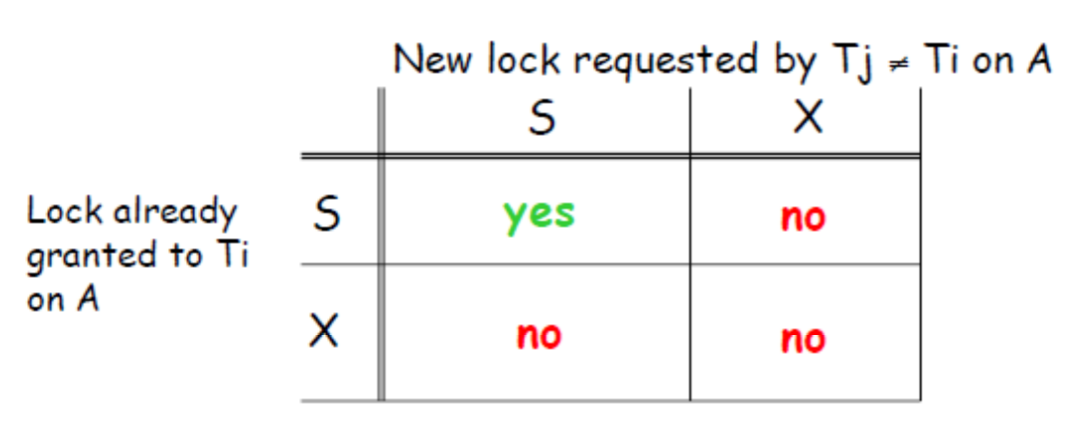
\includegraphics[scale=0.5]{Cattura4.png} 
\end{tabular}\\\\
There are several examples of \textbf{Block Ciphers} like:
\begin{itemize}
\item \textbf{DES}: (1976) with 64 \emph{bit block} and 56 \emph{bit key};
\item \textbf{RC-2}: (1987) designed by IBM, with 64 \emph{bit block} and variable \emph{key size}, vulnerable by an attack of $2^{34}$ chosen \emph{plaintexts};
\item \textbf{IDEA}: (1991) with 64 \emph{bit block} and 128\emph{ bit key}, strong, only weaker variants have been broken;
\item \textbf{Blowfish}: (1993) with 64\emph{ bit block} and variable\emph{ key size} from 32 up to 448 bits, still strong;
\item \textbf{RC-5}: (1994) with variable\emph{ block size} (32, 64, 128 bits) and variable \emph{key size} (0 to 2040 bits) and \emph{rounds} (0 to 255). 
\item \textbf{AES}: (2001) with 128 \emph{bit block} and 128-256 \emph{bit key}, very strong;
\end{itemize}
\clearpage
\subsubsection{AES}
\textbf{AES} or \textbf{Advanced Encryption Standard} is an \emph{algorithm} based on \emph{symmetric block cipher} in which we have a \emph{block size} of 128 bits and a \emph{key lengths} of 128, 192 or 256 bit that use \textbf{finite fields algebra}, and now have fun with \emph{settordici} mathematical formulas and almost useless concepts:
\begin{itemize}
\item A set $G$ with \emph{binary operation} $+$ (\emph{addition}) is called a \textbf{commutative group} if:
\begin{itemize}
\item $\forall a,b \in G, a+b \in G$;
\item $\forall a,b,c \in G, (a+b)+c = a+(b+c)$;
\item $\forall a,b \in G, a+b = b + a$;
\item $\exists 0 \in G, \forall a \in G, a + 0 = a$;
\item $\forall a \in G, \exists -a \in G, a + (-a) = 0$;
\end{itemize}
\item Let $(G,+)$ be a group, then $(H,+)$ is a\textbf{ sub-group} of $(G,+)$ if it is a group and $H\subseteq G$;
\begin{itemize}
\item The \emph{Theorem of Lagrange} says that: if $G$ is finite and $(H,+)$ is a \emph{subgroup} of $(G,+)$ then $|H|$ divides $|G|$;
\end{itemize}
\item Two natural $a$ and $b$ are said to be \textbf{congruent modulo} $n$ (with $n$ a positive integer):\\ $a \equiv b (mod\; n)$ if:
\begin{itemize}
\item If $|a-b|$ is multiple of $n$ or the integer division of $a$ and $n$ and of $b$ and $n$ yield the \emph{same remainder};
\item The \emph{congruence relation} is \emph{reflexive}, \emph{symmetric} and \emph{transitive}, hence it is an \emph{equivalence relation};
\item The \emph{quotient set} $Z_n$ is the set of $n$ classes of \emph{equivalence congruent} to $0, 1,... n-1$: $-1 \equiv n-1 (mod\; n), -2\equiv n-2(mod\; n),$ etc..;
\item The properties of \textbf{congruence} are:
\begin{itemize}
\item \textbf{Invariance over addition}:
\\ $a \equiv b \cdot (mod\; n)\;\; \Leftrightarrow \;\; (a+c) \equiv (b+c) \cdot (mod\; n)\; \;\;\;\forall \; a,b,c \in \mathbb{N}, \forall \; n \in \mathbb{N}_0$
\item \textbf{Invariance over multiplication}: 
\\ $a \equiv b \cdot (mod\; n)\;\; \Leftrightarrow \;\; (a\times c) \equiv (b\times c) \cdot (mod\; n)\; \;\;\;\forall \; a,b,c \in \mathbb{N}, \forall \; n \in \mathbb{N}_0$
\item \textbf{Invariance over exponentiation}: 
\\ $a \equiv b \cdot (mod\; n)\;\; \Leftrightarrow \;\; a^k \equiv b^k \cdot (mod\; n)\; \;\;\;\forall \; a,b,k \in \mathbb{N}, \forall \; n \in \mathbb{N}_0$
\end{itemize}
\end{itemize}
\item Let's $a^n$ denote $a + a +\; ... \; +a$ for $n$ times (\emph{Why $a^n$ and not $\sum_{n}a$? Only D'Amore knows, we spent two days wondering why the fuck he used this notation}), we say that $a$ is \textbf{of order} $n$ if $a^n=0$:
\begin{itemize}
\item For any $m<n, a^m \neq 0$ then all elements of finite groups have \textbf{finite order}, $a^n=1$ for \emph{multiplicative operator} (where $a^n$ denotes $a \cdot a\times\;...)$;
\item $Z_m$ is the set of \emph{natural numbers} $mod\; m$ and the elements of $Z_m$ are the classes of \emph{equivalence} of \textbf{congruent integers};
\item $Z_m^{*}$ is the set of \emph{natural numbers} $mod\; m$ that are \textbf{coprime} to $m$, the \textbf{multiplicative group} of $Z_m$;
\item $\phi(m)$ is the \textbf{Euler's totient function} and it's equal to $= |Z_m^{*}|$;
\item The \textbf{Euler Theorem} says that for all $a$ in $Z_m^{*}, a^{\phi(m)} = 1 \cdot mod\; m$ so we have:
\\ $a^{k \cdot \phi (m) + 1} = a\times mod\; m,\; k \geq 0$;
\begin{itemize}
\item We can also extend it to $Z_m$ where $m=pq$ and $p,q$ are \textbf{prime number} and we have:
\\ $a^{k \cdot \phi (m) + 1} = a\times mod\; m,\; k \geq 0$;
\end{itemize}
\item \emph{Quindi in poche parole, $Z_m$ è il set dei numeri naturali congruenti in modulo ai numeri che vanno da 0 a a $m-1$, $Z_m^{*}$ è il subset di $Z_m$ considerando solo i numeri coprimi con $m$ (due numeri sono coprimi se non hanno nessun divisore comune apparte 1), 
la funzione toziente di eulero è la funzione che restituisce il numero di interi coprimi tra 1 e il numero $m$ tipo $\phi(8)=4$ perchè $1,3,5,7$ sono coprimi)};
\end{itemize}
\item Let $G$ be a \textbf{group} and $a$ an element of order $n$, the set: $ \langle a \rangle = \{ 1,a,...\;,a^{n-1} \}$ is a \textbf{sub-group} of $G$, $a$ is called the \textbf{generator} of $\langle a \rangle$ (it's the number from which we can generate all the \emph{elements} of the \emph{subgroup}). If $G$ is \emph{generated} by $a$ then $G$ is called \textbf{Cyclic}, and $a$ is the \textbf{primitive element} of $G$. 
\begin{itemize}
\item The \emph{theorem} says that for any \emph{prime number} $p$ the \textbf{multiplicative group} of $Z_p^*$ is cyclic; 
\end{itemize}
\item A set $F$ with two \emph{binary operations} $+$ \emph{addition}, and $\times$ (or $\cdot$) \emph{multiplication} is called a commutative \textbf{ring} with identity if:
\begin{figure}[H]
  \centering
  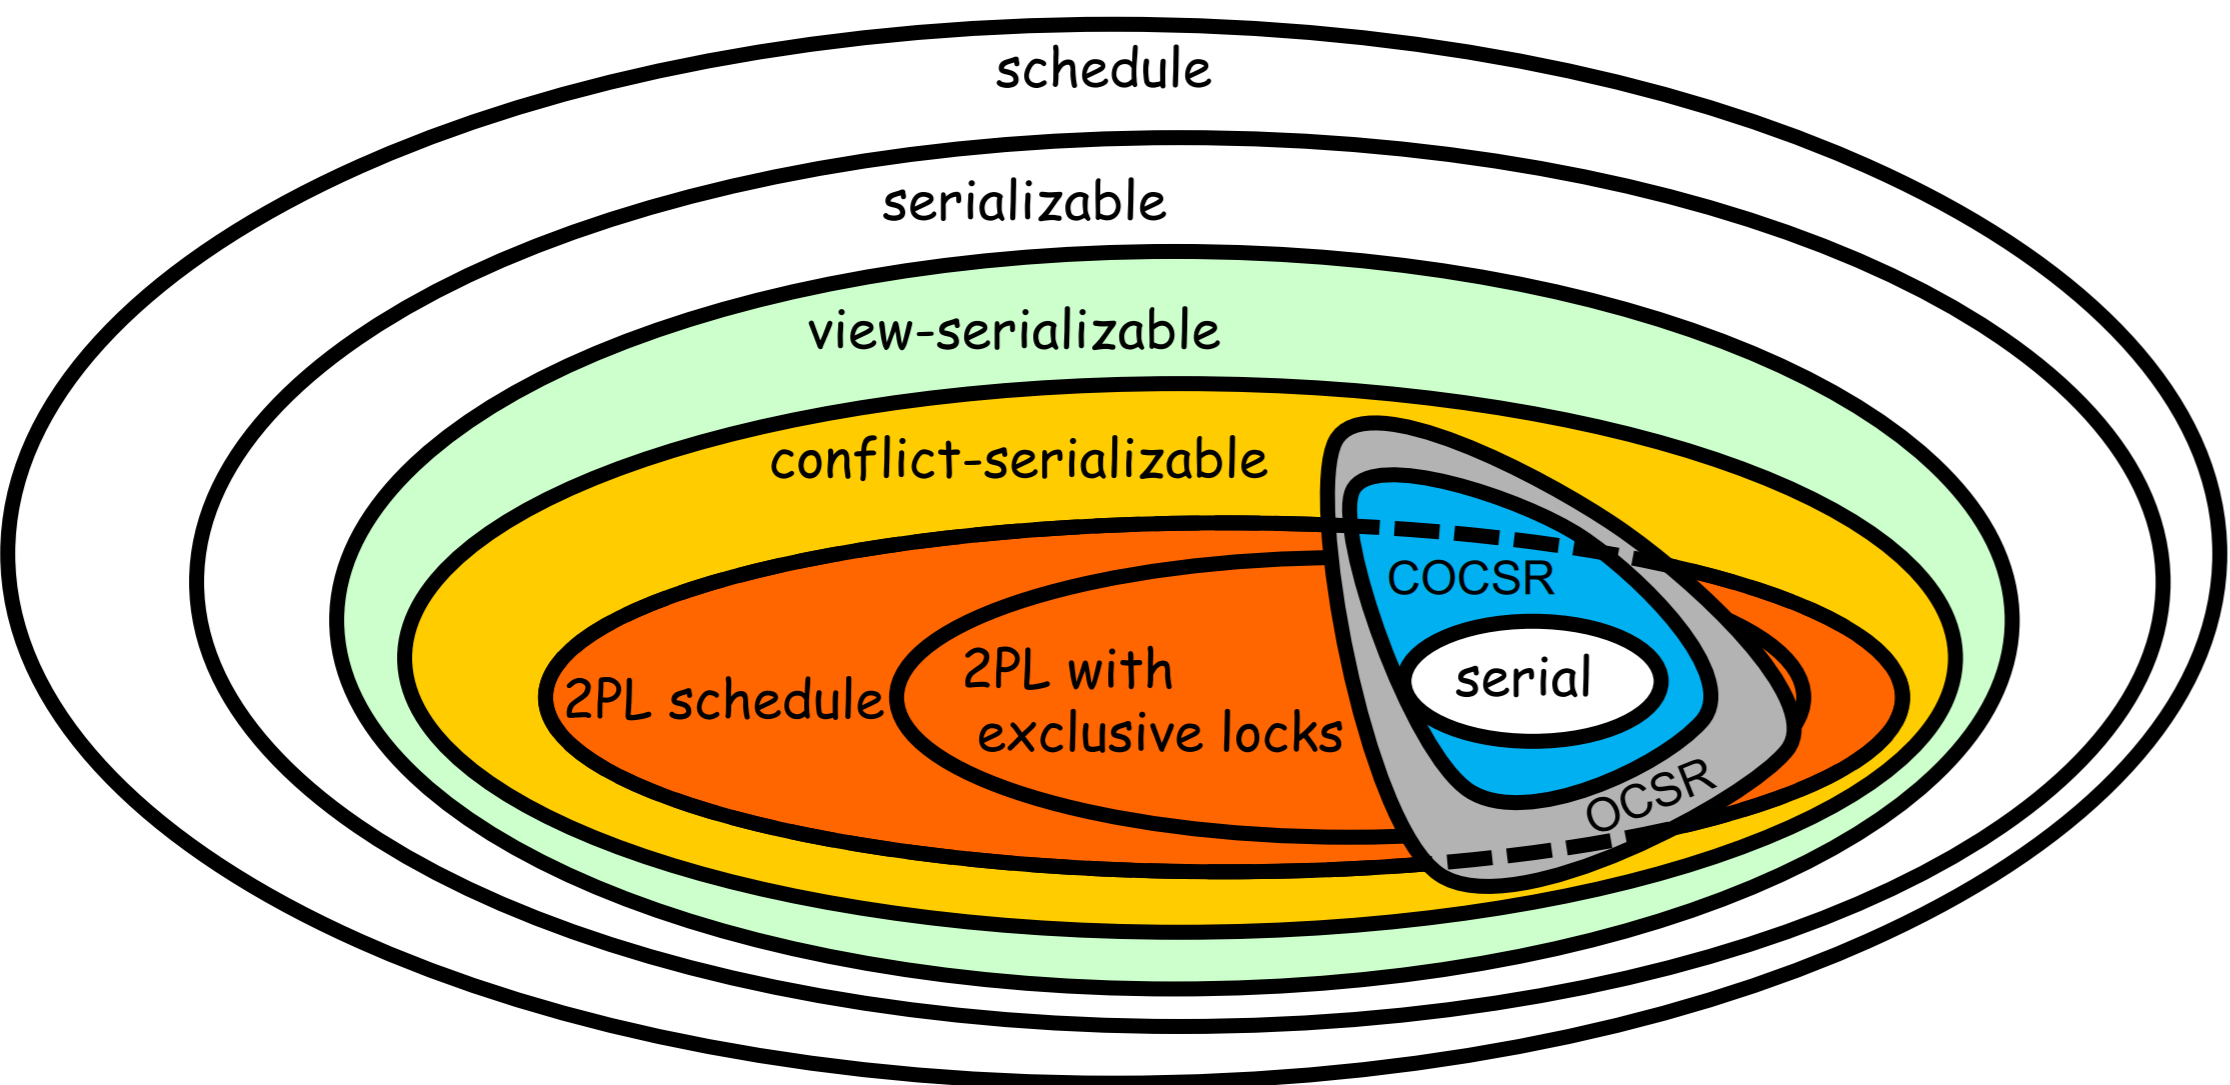
\includegraphics[scale=0.9]{cattura5.png}
\end{figure}
\item A set $F$ with two \emph{binary operations} $+$ \emph{addition}, and $\times$ (or $\cdot$) \emph{multiplication} is called a commutative \textbf{field} if:
\begin{figure}[H]
  \centering
  \includegraphics[scale=0.9]{cattura6.png}
\end{figure}
\begin{itemize}
\item A \textbf{field} is a \emph{commutative ring} with \emph{identity} where each non-zero element has a \emph{multiplicative inverse}. $(F,+)$ is a \textbf{commutative (additive) group} and $(F \setminus \{0\}, \cdot)$ is a \textbf{commutative (multiplicative) group} (with $\cdot$ distributive over $+$)
\end{itemize}
\item Let $f(x) = a_0 + a_1 \cdot x + ...\; + a_n \cdot x^n$ be a \textbf{polynomial} of \emph{degree} $n$ in one \emph{variable} $x$ over a \emph{field} $F$, the \textbf{theorem} says that $f(x) = 0$ has almost $n$ solution in $F$. It's important to note that this \emph{theorem} doesn't hold over \emph{rings with identity}. 
\begin{itemize}
\item Let $f(x) = a_0 + a_1 \cdot x + ...\; + a_n \cdot x^n$ and $g(x) = b_0 + b_1 \cdot x + ...\; + b_m \cdot x^m$ two \emph{polynomials} over $F$ such that $m \leq n$. There is a \emph{unique polynomial} $r(x)$ of degree $<m$ such that: $f(x) = h(x) \cdot g(x) + r(x)$ where $r(x)$ is called the \textbf{remainder} of $f(x)$ \textbf{modulo} $g(x)$;
\end{itemize}
\item A field $(F,+,\cdot)$ is called a \textbf{finite field} if the set $F$ is \emph{finite}. 
\begin{itemize}
\item The \emph{theorem} says that for every \textbf{prime power} $p^k$ with $k=1,2,...$ there is a \textbf{unique finite field} containing $p^k$ elements. These field are called \textbf{Galois Fields} and are denote with $GF(p^k)$. There aren't \emph{finite filed} with other \emph{cardinalities}. 
\item \emph{Polynomial equations} and \emph{factorizations} in \emph{finite fields} can be different than over the \emph{rationals};
\item A \emph{polynomial} is \textbf{irreducible} in $GF(p)$ if doesn't \emph{factor} over $GF(p)$, otherwise is \emph{reducible}. 
\end{itemize}
\item For a \emph{theorem}: let $f(x)$ be an \textbf{irreducible polynomial} of \emph{degree} $k$ over $Z_p$, the \emph{finite field} $GF(p^k)$ can be realized as the set of \textbf{degree} $k-1$ \textbf{polynomials} over $Z_p$, with \emph{addition} and \emph{multiplication} done \emph{modulo} $f(x)$;
\begin{itemize}
\item By the \emph{theorem} the \textbf{finite filed} $GF(2^5)$ can be realized as the set of \emph{degree} $4$ \emph{polynomials} over $Z_2$ with \emph{addition} and \emph{multiplication} done \emph{module} the \emph{irreducible polynomial} $f(x) = x^5+x^4+x^3+x+1$;
\item The \emph{coefficientes} of \emph{polynomials} over $Z_2'$ are $0$ or $1$, so a \emph{degree} $k$ can be written down by $k+1$ \emph{bits} so for example with $k=4$:
\begin{itemize}
\item $x^3+x+1 \rightarrow (0,1,0,1,1)$;
\item $x^4+x^3+x+1 \rightarrow (1,1,0,1,1)$;
\end{itemize}
\item The \emph{addiction} can be done through \textbf{XOR} since $1+1=0$:
\begin{figure}[H]
  \centering
  \includegraphics[scale=0.9]{cattura7.png}
\end{figure}
\item The \textbf{multiplication} is done by a \emph{Polynomial multiplication}, and then remainder \emph{modulo} the defining \emph{polynomial}. For small size \emph{finite field}, the \emph{lookup table} is the most efficient method for implementing \emph{multiplication}.
\end{itemize}
\end{itemize}
\clearpage
\hfill \break
Now finally the \textbf{AES}, that is a \emph{symmetric block cipher} with\emph{ key lengths} of $128,192$ or $256$ bit, and it's \emph{resistance} to all known \emph{attacks}. It's \emph{simple} and it's \emph{fast}, so it's very good for devices with limited \emph{computing power}. When we have \emph{Input} and \emph{Output block length} of 128 bits the \emph{State} of 128 bits we can arrange it as a\textbf{ 4-by-4 matrix of bytes}. 128 since we have 16 elements in the \emph{matrix} and each element is in byte that is formed by 8 bits so ($16 \cdot 8 = 128$). 
\begin{figure}[H]
  \centering
  \includegraphics[scale=0.7]{cattura8.png}
\end{figure}
When we have a \emph{key length} of 128,196,256 bits the \emph{Cipher Key Layout} that is arranged in a 4-by-$\frac{n}{32}$ matrix of \emph{bytes} (where $n= 128,196,256$ bit):
\begin{figure}[H]
  \centering
  \includegraphics[scale=0.65]{cattura9.png}
\end{figure}
The \emph{algorithm} at \textbf{high level} (\emph{without explanations in details that we will see later}) is:\\
\begin{algorithm}[H]
\renewcommand{\thealgorithm}{}
\caption{High level AES}
\begin{algorithmic}  
\STATE $AES(State,Key)$;
\STATE $KeyExpansion(Key,ExpandKey)$;
\STATE $AddRoundKey(Key,ExpandKey \left [0 \right ])$;
\STATE \textbf{for} ($i=1, i<R, i++$) \textbf{do}:
\STATE \hskip4.0em $Round(State,ExpandKey \left [i \right ])$;
\STATE $FinalRound(State,ExpandKey\left [R\right])$;
\end{algorithmic}
\end{algorithm}
\begin{tabular}{C{9cm}  L{10.5cm}}
So, this \emph{code} is repeated for each \emph{block} of the \emph{plain text} (each \emph{block} is of $128$ bits), so we start with a \emph{key} of $128$ bit, but before we start the \emph{rounds} (that are 10) since we don't want to use the same \emph{key} of 128 bits for all the different \emph{blocks}, we need to expand the \emph{key} in such a way for each \emph{block} we have a different \emph{key} of 128 bits. The \textbf{encryption} is done by following this scheme:
  & 
  \includegraphics[scale=0.5]{cattura10.png}
\end{tabular}
\clearpage
\hfill\break
We can see that every \emph{state} is done by the \textbf{encryption} of the \emph{precedent round} with the \emph{key extended} of the \emph{current block}. 128 bits AES uses 10 \emph{rounds}, in which the \emph{secret key} of 128 bits is expanded to 10 \emph{round keys} of 128 bits each. Each \emph{round} changes the \textbf{state}, then we \textbf{XOR} the \emph{round key}, if we have \emph{longer keys} we add one \emph{round} for every extra 32 bits. Now we will see in details what happen in each single \emph{round}, we start from the assumption that the \emph{plain text} that we are going to \emph{encrypt} is divided in \emph{state} of 128 bit and each \emph{state} can be divided in a matrix $4 \times 4$. We will \textbf{transform the state} by applying:\\
\begin{tabular}{C{9cm}  L{10.5cm}}
\begin{enumerate}
\item \textbf{Substitution};
\item \textbf{Shift rows};
\item \textbf{Mix columns};
\item \textbf{XOR round key};
\end{enumerate} &
\includegraphics[scale=0.7]{cattura8.png}
\end{tabular}
The \textbf{Substitution} operates on every \emph{byte} separately: $A_{i,j} \leftarrow A_{i,j}^{-1}$, so we apply a \emph{transformation} in place in every single \emph{block}, the operation is a \emph{multiplicative inverse} which is highly \emph{non-linear}. If $A_{i,j} = 0$ then we don't change $A_{i,j}$. It's important to note that the \textbf{substitution is invertible}.
\\\\
\begin{tabular}{C{9cm}  L{10.5cm}}
We will \textbf{Shift} each element of each \emph{row} to the \textbf{right}, 0 for the \emph{first row}, 1 for the \emph{second row}, 2 for the \emph{third row}, 3 for the \emph{fourth row}. This shift is invertible. 
  & 
  \includegraphics[scale=0.5]{cattura11.png}
\end{tabular}
In the \textbf{Mixing Columns} operation every state \emph{column} is considered as a \emph{Polynomial} over $GF(2^8)$, we will multiply with an \emph{invertible polynomial} $03 x^3+ 01x^2+01x+02(mod\; x^4 +1)$ the \emph{Inv} instead is $0B x^3 + 0D x^2+ 09x+0E$. \\\\
The \textbf{Key Expansion} instead will generate a different \emph{key} per \emph{round}, and need a $4\times4$ matrix of values per \emph{round}. It's based upon a \emph{non-linear transformation} of the \emph{original key}.\\\\
Breaking 1 or 2 \emph{rounds} of the \textbf{AES} is easy, actually is not known how to break 5 \emph{rounds}, and breaking the full 10 \emph{rounds} efficiently is considered impossible. \\\\
All \emph{block ciphers} operate on \emph{blocks} of \emph{fixed length} cause \emph{message} can be of any \emph{length} and because \textbf{encrypting} the same \emph{plaintext} under the same \emph{key} always produces the same \emph{output}. Several modes of \emph{operation} have been invented which allow \emph{block ciphers} to provide \textbf{confidentiality} for \emph{messages} of \emph{arbitrary length}. 
\subsubsection{ECB}
\textbf{ECB} or also called \textbf{Electronic Code Book} is an stream cipher in which we \emph{encrypt} each \emph{plaintext block} separately, and it's very simple and efficient, and also it's possible to implement it in a \emph{parallel way}. It doesn't conceal \textbf{plaintext patterns}, and it's possible to attack it with \emph{active attacks}, in fact \emph{plaintext} can be manipulated by removing, repeating or interchanging \emph{blocks}. 
\subsubsection{CBC}
\textbf{CBC} is the \textbf{Cipher Block Chaining}, created by \emph{IBM} in the 1976, is an \emph{asynchronous stream cipher}, in which \emph{errors} in one \emph{ciphertext block} will propagate, that conceals \emph{plaintext patterns} and there aren't \emph{parallel implementation}. \emph{Plaintext} cannot be easily manipulated and it's a standard in a lot of systems. In this cipher the previous \emph{ciphertext} is \textbf{XORed} with current \emph{plaintext} before \emph{encrypting} current \emph{block}. We use a \emph{seed} to start the process, and this \emph{seed} can be sent without \emph{encryption}. If we set $seed=0$, in most case is safe, but a \emph{random seed} is better.
\begin{figure}[H]
  \centering
  \includegraphics[scale=0.65]{cattura12.png}
\end{figure}
The \emph{CBC} can lead to \emph{problems}, in fact if there is a \textbf{transmission error} that changes just one bit of the $C_{i-1}$ then block $m_i$ changes in a \emph{predictable way} (and this is be used by an \emph{adversary}), but there are \emph{unpredictable changes} is $m_{i-1}$, so the \emph{solution} is to always use an \textbf{error detecting code}, that check the quality of the \emph{transmission}. The \emph{message} of the \emph{CBC} must be \textbf{padded} to a multiple of the \emph{cipher block size}, and in order to handle this issue we need to use the \textbf{Ciphertext Stealing}. A \emph{plaintext} can be \emph{recovered} from just two adjacent \emph{blocks} of \emph{ciphertext}, so as a consequence \emph{decryption} can be \textbf{parallelized}, in fact usually a \emph{message} in encrypted once, but \emph{decryption} is done many times. \\\\
\textbf{Ciphertext Stealing} is a general method that allows for processing of \emph{messages} that are not evenly divisible into \emph{blocks}, so it doesn't result in an expansion of the \emph{ciphertext}, it cost only in \emph{complexity}. It consists of altering processing of the last two \emph{blocks} of \emph{plaintext}, so it re-order the \emph{transmission} of the last two \emph{blocks} of \emph{ciphertext} and this method is suitable for \emph{ECB} and \emph{CBC}. 
\begin{figure}[H]
  \centering
  \includegraphics[scale=0.85]{cattura13.png}
\end{figure}
We can see that the last \emph{plaintext block} is not divisible for 128 (\emph{plaintext block size}, our \emph{block} is made by $n$ bits) so we fill the \emph{block} with all $0$, the \textbf{XOR} will be done only by the first $n$ bits of the \emph{previous ciphertext}. So during the \emph{decryption} the \emph{block} will be $\left [P_n^{*} \bigoplus C_{n-1}^* | C_{n-1}^{**} \right]$ so in order to get the original plaintext the result will be XORed with $C_{n-1}$ in this way we obtain: \[\left [P_n^{*} \bigoplus C_{n-1}^* | C_{n-1}^{**} \right] \bigoplus \left [  C_{n-1}^* | C_{n-1}^{**} \right ] = \left [ P_n^{*} |\; 000000... \right ]\]
\begin{itemize}
\item \textbf{Encryption}: 
\begin{itemize}
\item If the \emph{plaintext} length is not a multiple of the \emph{block size}, we will pad it with enough zero until it is.
\item We \emph{encrypt} the \emph{plaintext} using the \emph{Cipher Block Chaining mode};
\item We swap the last two \emph{ciphertext blocks} \emph{(? swap? where? in the figure there isn't any swap});
\item We truncate the \emph{ciphertext} to the length of the original \emph{plaintext}; 
\end{itemize}
\item \textbf{Decryption}:
\begin{itemize}
\item If the \emph{ciphertext} length is not a multiple of the \emph{block size}, (like $n$ bits short), then we pad the it with the last $n$ bits of the \emph{block cipher decryption }of the last full \emph{ciphertext block};
\item Swap the last two \emph{ciphertext blocks};
\item \emph{Decrypt} the \emph{ciphertext} using the \emph{Cipher Block Chaining mode};
\item We truncate the \emph{plaintext} to the length of the original \emph{ciphertext};
\end{itemize}
\end{itemize}
\subsubsection{PCBC}
\textbf{PCBC} is designed to extend or propagate a \emph{single bit error }both in \emph{encryption} and \emph{decryption} (before if there was a \emph{bit error} it will propagate to change all the \emph{message} here only a \emph{bit}). Here we have that the current \emph{plaintext} ($i$) before \emph{encryption} is \emph{XORed} with: $plaintext_{i-1} \bigoplus ciphertext_{i-1}$. In the \emph{decryption} will happen the same procedure, but the \emph{XOR} will happen after the \emph{decryption}, so since the \emph{decryption} need the \emph{plaintext} of the precedent \emph{block} is not possible anymore to do it in \emph{parallel} like in the \emph{CBC}. 
\begin{figure}[H]
  \centering
  \includegraphics[scale=0.8]{cattura14.png}
\end{figure}
On a \emph{message encrypted} in \textbf{PCBC mode}, if two adjacent \emph{ciphertext blocks} are exchanged, this doesn't affect the \emph{decryption} of \emph{subsequent blocks} (this doesn't happen to \emph{CBC}):
\begin{itemize}
\item $I_{i+2} = C_{i+1} \bigoplus (D_k (C_{i+1}) \bigoplus I_{i+1}) $;
\item $I_{i+1} = C_{i} \bigoplus (D_k (C_{i}) \bigoplus I_{i}) $;
\item $I_{i+2} = C_{i+1} \bigoplus (D_k (C_{i+1}) \bigoplus C_{i} \bigoplus D_k(C_i) \bigoplus I_i$
\end{itemize}
\subsubsection{CFB}
\textbf{CFB} is similar to \emph{CBC} but makes a \emph{block cipher} into an \textbf{asynchronous stream cipher}, so it supports some \emph{re-synchronizing} after error if the input to the encryptor is given by through a \textbf{shift-register}. In the \emph{encryptor} the \emph{plaintext} will be \emph{XORed} after applying the \emph{encrypt} (in the \emph{CBC} we do it before). Since the \emph{XOR} is done after \emph{encryption} we don't need anymore to pad last \emph{block} with 0 when the \emph{plaintext size} is not a multiple of the \emph{block size}:
\begin{figure}[H]
  \centering
  \includegraphics[scale=0.5]{cattura15.png}
\end{figure}
The \emph{decryption} can be made in \emph{parallel} since in order to obtain the \emph{plaintext} I only need the \emph{current block} and the precedent \emph{ciphertext}. If there is an error in the output of the \emph{encryption algorithm} this error will not be propagated in all the other \emph{blocks}, since it will only infect the current \emph{XOR} and the \emph{decryption} of the next \emph{block}. So \textbf{CFB} shares two advantages over \emph{CBC}, the \emph{block cipher} is only ever used in the \emph{encryption} direction and the \emph{message} doesn't need to be \emph{padded} to a multiple of the \emph{cipher block size}. \\\\
When we want to use a \textbf{CFB with shift register}, we start by initializing a \emph{shift register} the size of the \emph{block size} with the \emph{initialization vector}, this will be \emph{encrypted} with the \emph{block cipher} and the highest $s$ bits of the result are \emph{XORed} with $s$ bits of the \emph{plaintext} to produce $s$ bits of \emph{ciphertext}, that then we be \emph{shifted} in the \emph{register} and this \emph{process} will be repeated for the next $s$ bits of \emph{plaintext}. The \emph{decryption} is similar, we start with the \emph{initialization vector} we \emph{encrypt} and \emph{XOR} the high bits of the result with $s$ bits of the \emph{ciphertext} to produce $s$ bits of \emph{plaintext}, then we \emph{shift} the $s$ bits of the \emph{ciphertext} into the \emph{shift register} and \emph{encrypt} again:
\begin{figure}[H]
  \centering
  \includegraphics[scale=0.6]{cattura16.png}
\end{figure}
\subsubsection{OFB}
\textbf{OFB} or \emph{Output FeedBack} makes a \emph{block cipher} into a \textbf{synchronous stream cipher}, it generates \emph{keystream blocks} which are then \emph{XORed} with the \emph{plaintext blocks }in order to get the \emph{ciphertext}, similar to \emph{CFB} the \emph{plaintext} is \emph{XORed} after the \emph{encyrption}. Flipping a \emph{bit} in the \emph{ciphertext} produces a \emph{flipped bit} in the \emph{plaintext} at the same location, and this property allows many error correcting codes to function normally even when applied before \emph{encryption}. Contrarily to \emph{CFB} in output in the second \emph{block} I will not give the \emph{XORed} with the \emph{plaintext} but I will pass directly the \emph{encrypted output} of the algorithm, in this way if in the \emph{CFB} two \emph{blocks} of \emph{plaintext} are influenced by an \emph{error}, in \emph{OFB} only the \emph{current block} is influenced by the \emph{error}. 
\begin{figure}[H]
  \centering
  \includegraphics[scale=0.49]{cattura17.png}
\end{figure}
Since we have \emph{symmetry} of \emph{XOR operation} \textbf{encryption} and \textbf{decryption} are exactly the same:
\begin{itemize}
\item $C_i = P_i \bigoplus O_i$;
\item $P_i = C_i \bigoplus O_i$;
\item $O_i = E_k(O_{i-1}$;
\item $O_0 = IV$;
\end{itemize}
If $E_k$ is public, we need to \textbf{encrypt} the initial \emph{seed}. If $E$ is a \emph{cryptography function} that depends on a \emph{secret key} then the \emph{seed} can be in clear. The \emph{initial seed} must be modified for every new \emph{message}, in fact if the \emph{adversary} knows a \emph{pair message}, initial \emph{seed} then he can encode every \emph{message}. So with \textbf{OFB} we have:
\begin{itemize}
\item \emph{Synchronous stream cipher};
\item \emph{Errors} in \emph{ciphertext} do not propagate;
\item \emph{Pre-processing} is possible;
\item Conceals \emph{plaintext patterns};
\item No \emph{parallel implementation} known;
\item \emph{Active attacks} by manipulating \emph{plaintext} are possible;
\end{itemize}
\subsubsection{CTR}
\textbf{CTR} or \emph{Integer Counter Mode} turns a \emph{block cipher} into a \emph{stream cipher}, in fact it generates the next \emph{keystream block} by \emph{encrypting} successive values of a \emph{counter}. This \emph{counter} can be any \emph{function} which produces a \emph{sequence} which is guaranteed not to repeat for a long time. It has similar characteristics to \emph{OFB} but it also allows a \emph{random access property} during \emph{decryption}, so it's well suited to operation on a \emph{multi-processor machine} where \emph{blocks} can be \emph{encrypted} in \emph{parallel}. The generation of each \emph{ciphered block} is independent from any other \emph{blocks} since we use a different \emph{seed} for each \emph{block}. 
\begin{figure}[H]
  \centering
  \includegraphics[scale=0.8]{cattura18.png}
\end{figure}
Of course we have problems if we repeat the \emph{seed} like \emph{OFB}. When we use \emph{CTR} we can \emph{decrypt} the \emph{message} starting from \emph{block} $i$ for any $i$, since we don't need to \emph{decrypt} from the first \emph{block}. 
\subsubsection{Initialization Vector}
Most \emph{modes} (except \emph{ECB}) require an \textbf{Initialization vector}, or \textbf{IV}, that is a sort of \emph{dummy block} used to kick off the \emph{process} for the first real \emph{block}. It doesn't need to be secret in most case but it's important that it is never reused with the same \emph{key}, in fact, in \emph{CBC} and \emph{CFB}, reusing \emph{IV} leaks some information about the first \emph{block} of \emph{plaintext}. In \emph{CBC} mode the \emph{IV} must be unpredictable in \emph{encryption time}. For \emph{OFB} and \emph{CTR} reusing an \emph{IV} completely destroys \emph{security}. 
\subsubsection{Strengthening a cipher}
There are two ways in order to \textbf{strengthening a cipher}:
\begin{itemize}
\item \textbf{Key Whitening}:
\begin{itemize}
\item Consist of steps that combine the \emph{data} with portions of the \emph{key} (usually by using \emph{XOR}) before the \emph{first round} and after the \emph{last round} of \emph{encryption};
\end{itemize}
\item \textbf{Iterated Ciphers} (\emph{Triple DES, 3-DES}):
\begin{itemize}
\item In which the \emph{plaintext} undergoes \emph{encryption} repeatedly by \emph{underlying cipher}, in which ideally we use a different \emph{key} so we have for \emph{triple cipher}:
\begin{itemize}
\item $C = E_{k_1}(E_{k_2}(E_{k_1}(P)))$ called EEE mode;
\item $C = E_{k_1}(D_{k_2}(E_{k_1}(P)))$ called EDE mode;
\end{itemize}
\item So we use \emph{three algorithms} of \emph{encryption} or \emph{two algorithm} of \emph{encryption} and one of \emph{decryption}. Sometimes only \emph{two keys} are used in \emph{3-DES}, and identical key must be at beginning and end. 
\end{itemize}
\end{itemize}
Since the \emph{goal} of the \textbf{adversary} it to find the \emph{secret }key, the \textbf{double DES} cannot be used, in fact if we have a \emph{double cipher} with two different \emph{keys} the \emph{adversary} can use the \textbf{meet-in-the-middle attack}. If fact if \emph{plaintext/ciphertext} pairs are known, we have $2^n$ \emph{encryption} and $2^n$ \emph{decryption} so $2$ keys of $n$ bits. So it's possible to try all possible $2^n$ \emph{encryptions} of the \emph{plaintext} and all possible $2^n$ \emph{decryptions} of the \emph{ciphertext}. In other words, the presence of two different \emph{keys} is represented as a \emph{function} $h(x) = g(f(x))$, and the \emph{middle attack} try to \emph{map} the \emph{co-domain} given the \emph{domain} of the \emph{function} $f$ with the \emph{counter-image} of the\emph{ co-domain} of the $g$ function, so if initially you think to have a set of $2^{2n}$ keys in reality the attacker will make $2^n$ attempts, cause assuming that the \emph{adversary} knows some \emph{ciphertexts} $C$ and some \emph{plaintexts} $P$, the attacker can \textbf{in parallel} \emph{encrypt} $P$ and \emph{decrypt} $C$ trying to find some correspondences and if he find them he found the \emph{key}.  \\\\
It's even possible to use the \emph{triple encrypting} with the \textbf{CBC}, and this can be done in two ways, by \textbf{external CBC}, in which we use a \emph{triple encoding}, or \textbf{internal CBC}, in which we have an \emph{encryption} after a \emph{decryption} (with a different key) and another \emph{encryption}. 
\section{Data Integrity \& Authentication}
The \emph{goal} is to ensure the \textbf{integrity} of \emph{messages} even in presence of an \emph{active adversary} who sends own \emph{messages}. It's important to note that \emph{authentication} is orthogonal to \emph{secrecy} (so they are independent between each other), so the \emph{secrecy} of a \emph{messages} doesn't not imply that the \emph{sender} of the \emph{message} is actually the one with who you think you are communicating. 
\begin{figure}[H]
  \centering
  \includegraphics[scale=0.8]{cattura19.png}
\end{figure}
\subsection{MAC}
The \textbf{authentication algorithm} is called $A$, the \textbf{verification algorithm} is called $V(accept/reject)$, the \textbf{authentication key} is $k$, and the \textbf{message space} is usually a \emph{binary strings}. Every \emph{message} between Alice and Bob is a \emph{pair}: $(m,A_k(m))$, where $A_k(m)$ is called the \textbf{authentication tag} of $m$. The \emph{authentication algorithm} is called \textbf{MAC}, \emph{Message Authentication Code}, in fact $A_k(m)$ is frequently denoted as $MAC_k(m)$ and the \emph{verification} is done by executing \emph{authentication} on $m$ and comparing it with $MAC_k(m)$. The \emph{security requirement} is that \emph{adversary} can't construct a new \textbf{legal pair} $(m,MAC_k(m))$ even after seeing a $(m_i,MAC_k(m_i))$. The \emph{output} should be as short as possible and the \emph{MAC function} is not 1-to-1. \\\\
The \textbf{adversary} knows the \emph{MAC algorithm}, knows \emph{plaintext pairs} $(m,MAC_k(m))$, and knows \emph{chosen plaintext} (unrealistic) so choose $m$ get $MAC_k(m)$ and the \textbf{goal} is given $n$ \emph{legal pairs} find a \textbf{new legal pair} $(m,MAC_k(m)$ \textbf{efficiently} and with \textbf{non negligible probability} (so, \emph{non sparato a cazzo}). \\\\
In practice \textbf{MAC} used are based on two types:
\begin{itemize}
\item \textbf{MAC based on CBC encryption}, so uses a block cipher (slow);
\item \textbf{MAC based on cryptographic hash functions}, no restriction on export (fast);
\end{itemize}
\subsection{MAC based on CBC}
In CBC the previous ciphertext is XORed with current plaintext before encrypting the current block. With CBC with MAC's we start with the all zero seed, and given a message $m$ consisting of $n$ blocks $M_1, M_2, ...\;, M_n$ we apply CBC using a secret key $k$. 
\begin{figure}[H]
  \centering
  \includegraphics[scale=0.8]{cattura20.png}
\end{figure}
So this produces $n$ \emph{ciphertexts block} $C_1, C_2, ... \;, C_n$ and we decide that $MAC_k(m)= C_n$, so we take only the last \emph{ciphertext}. This is a very \emph{secure} way, but it's\textbf{ very slow} since the \emph{encryption} cannot be done in \emph{parallel}. A \textbf{pseudo random function}, it's a function that looks random, and a good \emph{encoding scheme} transforms the \emph{message} in an apparently \emph{random string}. If $A_k$ is a \emph{pseudo random function}, the \textbf{fixed length CBC MAC} is resilient to forgery. \emph{CBC MAC} is secure for \emph{fixed-length messages} but insecure for \emph{variable-length messages}, in fact, if an \emph{attacker} knows correct \emph{message-tag pairs} $(m,t)$ and $(m^{'},t^{'})$ then can generate a \emph{longer messages} $m^{''}$ whose CBC-MAC will also be $t^{'}$:
\begin{itemize}
\item \emph{XOR first block} of $m^{'}$ with $t$ and then \emph{concatenate} $m$ with the modified $m^{'}$;
\item $m^{''} = m\; |\; m^{'}_1 \bigoplus t \;|\; m^{'}_2 \;|\; ... \; |\; m_x^{'}$;
\end{itemize}
So in this way the \emph{tuple} sent by the \emph{attacker} will be accepted by the \emph{receiver}. A solution in order to avoid this attack is to produce \emph{ciphertext blocks} with a \emph{different key}, not the same of the \emph{key} of the \emph{authentication tag.} 
\subsection{MAC based on hash functions}
The \textbf{hash functions} are \emph{functions} in which we map \emph{large domains} to \emph{smaller ranges}, used extensively for \emph{searching} (\emph{hashing tables}), we have the problem of \emph{collisions} that are resolved with \emph{chaining} or \emph{double hashing}, etc. The goal is to compute \emph{MAC} of a \emph{message} by using an \emph{hash function} $h$ for a \emph{message} $m$ with a \emph{secret key} $k$, so \emph{MAC} must be a \emph{function} of the \emph{key} and the \emph{message}. For example $MAC_k(m) = h(k \parallel m)$. 
\begin{itemize}
\item An \emph{hash function} $h: D \rightarrow R$ is called \textbf{weakly collision resistant} for $x \in D$ if it's hard to find $x \neq x^{'}$ such that $h(x^{'}) = h(x)$;
\item An \emph{hash function} $h: D \rightarrow R$ is called \textbf{strongly collision resistant} if it's hard to find $x, x^{'}$ such that $x \neq x^{'}$ but $h(x^{'}) = h(x)$;
\end{itemize}
The difference between the two definitions is that in the \emph{weakly} the \emph{element} is given, instead in the \emph{strongly} we need to find two \emph{elements}. It's important to note that $Strong \Rightarrow Weak$ and the proof is:
\begin{itemize}
\item If I have an \textbf{non-weak} I can use an \emph{algorithm} that takes $x$ as \emph{input} and returns $x^{'}$ that \emph{collide} with $x$. I can also use an \emph{algorithm} that finds both $(x,x^{'})$ that \emph{collide}, so it's \emph{not strong};
\end{itemize}
The \textbf{birthday paradox} says: if 23 people are chosen at random the \emph{probability} that two of them have the same birthday is $>0.5$. In other words, if $h: D \rightarrow R$ if we choose randomly $1.1774|R|^{1/2}$ \emph{elements} of D the probability that two of them \emph{collide} is $>0.5$. This means that if we have $2^n$ possible \emph{message tags}, we have to try only $2^{n/2}$ \emph{messages} to have a\textbf{ collision probability} $>0.5$. The \textbf{Birthday Attack} uses this paradox, in fact given a \emph{function} $f$ find two different \emph{input} $x_1, x_2$ such that $f(x_1) = f(x_2)$ with a 64-bit hash, would take at least $5.38\times 10^9$ attempts to generate a \emph{collision} by using \emph{brute force}. This limit is called \textbf{birthday bound}.\\\\
\textbf{Cryptographic hash function} are \emph{hash functions} that are \emph{strongly collision resistant}, they don't use a \emph{secret key}, usually they are defined by a \emph{compression function} that maps $n$ bits in $m$ bits with $m<n$. We talk about \textbf{Merkle-Damgard construction}:
\begin{figure}[H]
  \centering
  \includegraphics[scale=0.8]{cattura21.png}
\end{figure}
A mode of \emph{operation} that returns a \textbf{digest} from a \emph{document}. $f$ is an \emph{hashing function} that has a \emph{domain} of $n$ bits and a \emph{codomain} of $m$ bits. This means that the \emph{message} has to be divided in \emph{blocks}. In the figure we can see that the \emph{block size} is $n-m$. To avoid \emph{birthday attacks} we simply have to define a large \textbf{codomain size}, (more than 160 bits) in such a way \emph{brute-force }is not feasible. \clearpage
\hfill \break
The \textbf{Keyed Hashing Functions} have the goals to combine \emph{messages}, \emph{keys} and \emph{hash functions} in order to produce \emph{MAC}. These provide both \emph{data integrity} and \emph{authentication}. We have to mix the \emph{message} and the \emph{key}, in a concatenation, and then use \emph{hash-based algorithms}. We have different ways:
\begin{itemize}
\item $MAC_k(m) = h(k\parallel m) $, \textbf{insecure}, cause it suffers the \emph{length-extension attack}, in which an \emph{attacker} can add extra bits to the \emph{message} and compute correct \emph{MAC};
\item $MAC_k(m) = h(m\parallel k) $, \textbf{insecure}, cause if \emph{attacker} finds a \emph{collision} in the \emph{hash function} (\emph{birthday attack}) between two \emph{messages}, then he will know two \emph{messages} with the same \emph{MAC} for all \emph{keys};
\item $MAC_k(m) = h(k\parallel m\parallel k)$, \textbf{secure};
\item $MAC_k(m) =$ first bits of $h(k\parallel m)$ or $h(m\parallel k)$, \textbf{secure};
\end{itemize}
\subsubsection{SHA-1}
As any \emph{hash function}, \textbf{SHA-1} produces a \emph{digest} of fixed length (160 bit) starting from a \emph{message} of variable length, that will be \emph{padded}. There are 4 phases:
\begin{itemize}
\item \textbf{Padding}:
\begin{itemize}
\item In this phase, \emph{padding bytes} are added to the original \emph{message} until it is congruent in bit to $448\; mod\; 512$;
\end{itemize}

\item \textbf{Adding length}:
\begin{itemize}
\item To the \emph{final message} (\emph{original message} plus \emph{padding}) we add an \emph{unsigned integer} of 64 bits that denoting the \emph{full length} of the \emph{message}, so we obtain a \emph{message} that is multiple than 512 bit;
\end{itemize}
 \begin{figure}[H]
  \centering
  \includegraphics[scale=0.9]{cattura22.png}
\end{figure}
\item \textbf{MD buffer initialization}:
\begin{itemize}
\item A 160 \emph{bit buffer} is subdivided in 5 \emph{registers} of 32 bits each one that are:
\begin{itemize}
\item $A=67452301$;
\item $B = EFCDAB89$;
\item $C = 98BADCFE$;
\item $D = 10325476$;
\item $E = C3D2E1F0$;
\end{itemize}
\end{itemize} 
\item \textbf{Block Elaboration}:
\begin{itemize}
\item  Now that we have the \emph{5 registers} we can start computing \emph{hashing}. The \emph{complete message} is subdivided into several \emph{blocks} of 512 bits. The core of the \textbf{SHA-1} \emph{algorithm} is the \textbf{compression function} which is composed by 4 \emph{cycles} of 20 \emph{steps} each one. Starting from the \emph{first block} of 512 bits we give as \emph{input} to the \emph{compression function} the \emph{block}, a \emph{constant} $k$, and the values of the \emph{five registers}. At the end of the \emph{compression function} a new state of the \emph{five registers} is observed, and we go on with the next \emph{block}. When the \emph{last block} of the \emph{message} is compressed the \emph{final values} of the \emph{five register} will be summed to the initial values of the \emph{five register} and the resulting values creates the \textbf{digest} that will be composed as $A|B|C|D|E$. 
\begin{figure}[H]
  \centering
  \includegraphics[scale=0.7]{cattura23.png}
\end{figure}
\end{itemize} 
\end{itemize}
\subsubsection{HMAC}
It's a \textbf{Keyed Hashing MAC} which uses a pattern similar tot last one we listed. It's a \emph{mode of operation} that we can use inside an \emph{hash-algorithm,} so it's not an \emph{hash-algorithm}. \emph{HMAC} receives as input a \emph{message} $m$ a \emph{key} $k$ and an \emph{hash function} $h$ and then it computes:
\[ HMAC_k(m,h) = h(k \bigoplus opad \parallel h (k \bigoplus ipad \parallel m))\]
Where \emph{opad} is the \textbf{outer padding}: $0x5c5c...5c$, and \emph{ipad}, \textbf{inner padding}: $0x3636...36$ both long as a \emph{block}. \\\\
We can note that if two \emph{messages} collide in the \emph{inner hash} $h(k \bigoplus ipad \parallel m)$ they will collide for the whole \emph{hashing scheme}, cause the \emph{outer hash} adds the same stuff to both \emph{messages}. So, \emph{HMAC} still suffers the \textbf{birthday paradox}, but the \emph{adversary} cannot understand which are the \emph{colliding pairs}, in fact, he is able to find two strings which \emph{collide}, but since the \emph{adversary} doesn't know the \emph{key} $k$ he cannot retrieve the \emph{messages} of the strings. 
\subsubsection{AE}
\textbf{AE}, or \textbf{Authenticated Encryption}, is a form of \emph{encryption} which simultaneously assures the \emph{confidentiality} and the \emph{authenticity of data}, often is offered as single primitive in modern \emph{API}, and it makes \emph{chosen-ciphertext attack} less dangerous, since the \emph{attacker} is not able to choose a \emph{ciphertext} and present it to the \emph{decryption} in a proper way. There are three different approaches to \emph{AE}:
\begin{itemize}
\item \textbf{Encrypt-then-MAC (EtM) }:
\begin{itemize}
\item The most secure today, in which we use two \emph{different keys} $k_1$ and $k_2$ where the first one is used for the \emph{encryption}, the second is used to find the \emph{MAC} starting from the \emph{encrypted message};
\end{itemize}
\item \textbf{Encrypt-and-MAC (E\&M) }:
\begin{itemize}
\item \emph{Safety} has not yet been proven, in which the\emph{ same key} is used for the \emph{encryption} and in order to find the the \emph{MAC}, starting from the \emph{plaintext};  
\end{itemize}
\item \textbf{MAC-then-Encrypt (MtE)}:
\begin{itemize}
\item Proven to be \emph{secure} in specific setting, like in\emph{ E\&M }we use only one \emph{key}, but here first we generate the \emph{MAC} starting from the \emph{plaintext}, and after \emph{plaintext} and \emph{MAC} are \emph{encrypted} together with the \emph{key};
\end{itemize}
\end{itemize}
\begin{figure}[H]
  \centering
  \includegraphics[scale=0.7]{cattura24.png}
\end{figure}
\clearpage
\section{Public Key Cryptography}
We have seen a \emph{model} in which Alice and Bob share the same \emph{secret key} $k_{A,B}$, and it must be \emph{secretly generated} and \emph{exchanged} before using the \emph{communication channel}. Then in 1976, \emph{Diffie and Hellman} came up with with a great idea: the \textbf{Public Key Infrastructure}. It's a model that uses \textbf{asymmetric encryption}, where each part has \emph{two keys} $K_E$ and $K_D$ used for \emph{encrypting} and for \emph{decrypting}. They are \emph{asymmetric}, this means that once we \emph{encrypt} with a \emph{key}, we must \emph{decrypt} with the other \emph{key}, and it's important to note that one of the\emph{ two keys} is \emph{public} and the other is \emph{private}. The implementation where \emph{keys} are \emph{asymmetric} it's hard and there are several ways:
\begin{itemize}
\item \textbf{One Way Function}:
\begin{itemize}
\item Are \emph{functions} for which given the input it's \textbf{easy} to compute the \emph{output} (in \emph{polynomial time}), but given the \emph{output} is \textbf{difficult} to retrieve the \emph{input} that generated that \emph{output}. An example of such a \emph{function} is multiplication: given two numbers $p,q$ compute $N=p\times q$ it's easy but having $N$ it's hard to retrieve $p$ and $q$, the mathematical definition is:
\item A function $f: \{0,1\}^{*} \rightarrow \{0,1\}^{*}$ is \textbf{one-way} if $f$ can be computed in \emph{polynomial time}, but for every \emph{randomized polynomial time algorithm} $A$, and for every \emph{polynomial} $p(n)$ with sufficiently large $n$:
\[ Pr \left [ f(A(f(x))) = f(x) \right ] < \frac{1}{p(n)}; \]
\item So the \emph{function} must be \textbf{hard} to invert in the \emph{average case}, rather than \emph{worst-case} sens, and that the \emph{probability} to find the correct $x$ that returned $f(x)$ trough $A$, it's very small;
\item \emph{A very typical question in the exam is: SHA-1 is a one way function? The answer is yes, and we cannot use it to make encryption since it's not a one-to-one, since is not injective, if you don't know the key the ciphertext is hard to be inverted to find the plain text, you can brute force it but it's very hard;}
\end{itemize}
\item \textbf{Discrete Log}:
\begin{itemize}
\item Let $G$ be a \emph{finite cyclic group} with $n$ elements and $g$ a generator of G. Let $y$ be any element in $G$, then it can be written as $y= g^x$ for some integer $x$ (for example $Z_n$ of 14 is \{1,3,5,9,11,13\} then the \emph{generator} of this \emph{group} is $g=3$ cause from this value we get all the values of the \emph{group}: $3\; mod \;14 = 3, 3^2\; mod\; 14 = 9, etc$). Let $y = g^x$ and $x$ the \emph{minimal non negative integer} satisfying the equation, then $x$ is called \textbf{discrete log} of $y$ to base $g$;
\item Let $y= g^x\;mod\; p$ in $Z_p^{*}$ (set of \textbf{positive integers} less than $p$ and \textbf{coprime} to $p$):
\begin{itemize}
\item Given $x$ calculating $y= g^x\; mod\; p$ it's \textbf{easy and computable} in $O(log^3 P)$ steps;
\item Instead given $g, y$ and $p$ it's believed to be \textbf{hard} to retrieve $x$, the \textbf{discrete log};
\end{itemize}
\item So retrieving the \textbf{Discrete Log} is believed to be a \textbf{One Way Function}. 
\end{itemize}
\end{itemize}
\subsection{Public Exchange of Keys}
The \textbf{goal} is to have the possibility that two \emph{parties}, \emph{Alice and Bob}, who don't share any \emph{secret information}, could perform a \emph{protocol} in order to \textbf{derive} the same \emph{shared key}, without exchanging it in \emph{clear}. \emph{Eve}, the \emph{attacker}, that is listening, cannot obtain the new \emph{shared key} in \emph{polynomial time} (unless $P=NP$ \emph{fuori di testa zi}). This \emph{protocol} was created by Diffie and Hellman, and the idea is to use a \textbf{session key}, that is a \textbf{shared secret key}, used for a \emph{confidential conversation} for a certain period and then it's dropped. The protocol works as:
\begin{itemize}
\item The \textbf{public parameters} are: a \emph{prime} $p$, a number $g$ (possibly a \emph{generator} of $Z_p^{*}$), and it works better if $p$ is a\textbf{ safe prime}, a \emph{prime} number for which $p=2q+1$ where even $q$ is \emph{prime};
\item Alice chooses a value $a$ at random $\in \left [1,p-1 \right]$, and sends $g^a\; mod\; p$ to Bob.
\item Bob chooses a value $b$ at random $\in \left [1,p-1 \right]$, and sends $g^b\; mod\; p$ to Alice.
\item Both the parties computes the \textbf{shared key} $g^{ab} mod\; p$ in fact:
\begin{itemize}
\item Alice that holds $a$ computes $(g^b\; mod\; p)^a = (g^b)^a\; mod\; p = g^{ab}\; mod\; p$ (for the properties of \emph{mod}); 
\item Bob that holds $b$ computes $(g^a\; mod\; p)^b = (g^a)^b\; mod\; p = g^{ab}\; mod\; p$ (for the properties of \emph{mod});
\end{itemize}
\item So at the end they have the \textbf{same key};
\end{itemize}
This can be applied even to \emph{multiple parties}, of course the number of \emph{exchanged message} will increase. Despite 25 years this is still \textbf{secure}. At the end of the session the \emph{values} $a$ and $b$ are \emph{discarded}, so the \emph{Diffie-Hellman} achieves the \textbf{perfect forward secrecy}, that means that if an \emph{attacker} discovers secret information about a \emph{previous session} of \emph{message exchanging}, he cannot be able to retrieve any information for the next session of \emph{message exchanging}. The \emph{computation time} is $O(log^3 p)$. \\\\
\emph{Diffie-Hellman} is effective only against a \emph{passive adversary} (\textbf{sniffing}), instead suffers the \textbf{Man-In-The-Middle attack}, which is \emph{lethal} for this \emph{protocol} and the attacker can control the whole conversation.The \emph{attacker} makes \emph{independent connections} with the victims, and relays \emph{messages} between them, making them believe that they are talking directly to each other over a \emph{private connection}.\\\\
\begin{tabular}{C{9cm}  L{10cm}}
Eve \textbf{intercepts} Alice's \emph{public value} and sends her own \emph{public value} to Bob. When Bob transmits his \emph{public value}, Eve substitutes it with her own and sends it to Alice. Eve and Alice thus agree on one \textbf{shared key} and Eve and Bob agree on another \textbf{shared }key. After this \emph{exchange}, Eve simply decrypts any \emph{messages} sent out by Alice or Bob, and then \emph{reads} and possibly \emph{modifies} them before \emph{re-encrypting} with the appropriate \emph{key} and transmitting them to the other party. This \emph{vulnerability} is present because \textbf{Diffie-Hellman key exchange} doesn't \textbf{authenticate} the participants.
 & \includegraphics[scale=0.4]{cattura25.png}
\end{tabular}\\\\
In order to have a secure \textbf{DH protocol}, an \textbf{authentication system} must be added, in fact, most \emph{cryptographic protocols} include some form of \emph{endpoint authentication} to prevent this \emph{attack}. \emph{Key Enchange} is used by \textbf{VPN}, that are made by two \emph{protocols}, an \emph{Handshake Protocol}, in which we have a \emph{key exchange} between parties sets \emph{symmetric keys}, and a \emph{Traffic Protocol}, in which \emph{communication} in \emph{encrypted} and \emph{authentication} is made by \emph{symmetric keys}. 
\section{RSA}
RSA is the implementation of the idea of Diffie and Hellman on the Public Key Infrastructure, and these implementation need some mathematical properties:
\subsection{Math considerations}
\begin{itemize}
\item \textbf{Multiplicative Group} $Z_{pq}^{*}$:
\begin{itemize}
\item Let $p$ and $q$ be two large \emph{prime numbers}, and let's denote their \emph{product} with $N=pq$, $N$ it's not \emph{prime}, but it's a \textbf{semiprime} (a product of two primes);
\item The \textbf{multiplicative group} $Z_{pq}^{*}= Z_N^{*}$, contains all \emph{integers} in the range $\left[1,pq-1\right]$ that are \textbf{coprime} to both $p$ and $q$. It's \textbf{cardinality} it's not $pq-1$ cause N it's not \emph{prime}. There are $(p-1)$ multiples of $q$ and $(q-1)$ multiples of $p$ so the \emph{cardinality} (the size of the group) is:
\[ \phi(pq) = |Z_{pq}^{*}| = pq-1 - (p-1) - (q-1) = pq - (p+q) +1 = (p-1)(q-1); \]
\item So for the \textbf{Euler theorem}, we have that for every $x \in Z_{pq}^{*}, x^{(p-1)(q-1)} = 1$;
\end{itemize}
\item \textbf{Exponentiation in} $Z_{pq}^{*}$:
\begin{itemize}
\item We notice that not all the integers between $\left[1,pq-1\right]$ are in $Z_{pq}^{*}$, this means that each element in that range doesn't have necessarily have a \emph{unique inverse} in $Z_{pq}^{*}$. We want an $e$ that is in the range $\left [1, (p-1)(q-1) \right ]$, such that the power operation $x \rightarrow x^e$ is a \textbf{one-to-one operation} in $Z_{pq}^{*}$ (\emph{every element of the \emph{function's codomain} is the image of at most one element of its \emph{domain}});
\item Since an element in the range $\left[1,pq-1\right]$ can have more than one inverse in $Z_{pq}^{*}$, then we cannot choose $e$ at random;
\item If we set $e$ as a coprime to $(p-1)(q-1)$, then since the $gcd(e, (p-1)(q-q)) = 1$ (\emph{from the definition of coprime, gcs is mcd}), $e$ has a \textbf{modular multiplicative inverse} called $d$ of $mod\; (p-1)(q-1)$ (\emph{a number for which} $(e \cdot d)\; mod\; (p-1)(q-1) = 1$);
\item Then we have that $ed= 1 + C(p-1)(q-1)$ where $C$ is a constant;
\item Let $y=x^e$, then:
\[y^d = (x^e)^d = x^{1+C(p-1)(q-1)} = x^1\cdot x^{C(p-1)(q-1)} = x(x^{(p-1)(q-1)})^C = x \cdot 1 = x;\]
\item This means that the power $y \rightarrow y^d$ is the inverse of $x \rightarrow x^e$, so $x \rightarrow x^e$ is a\textbf{ one-to-one operation}.
\end{itemize}
\end{itemize}
\subsection{RSA Protocol}
\begin{itemize}
\item Choose two \emph{prime numbers} $p$ and $q$ and let $N=pq$ be their \emph{product};
\item Choose an $e$ such that $1<e<\phi(N)$ and $gcd(e, \phi(N))=1)$ so $e$ is \emph{coprime} with $\phi(N)$;
\item Let $d$ such that $de \equiv 1\; mod\; \phi(N)$, so $d$ is the \emph{modular multiplicative inverse}; 
\item Then the public key is $(e,N)$;
\item The private key is $(d,N)$;
\item We will encrypt $M \in Z_n$ by $C = E(M) = M^e\; mod\; N$;
\item We will decrypt $C \in Z_n$ by $M = D(C) = C^d\; mod\; N$;
\item Decryption is valid since:
\begin{itemize}
\item If $ed= 1 \mod \phi$ then there is an integer $k$ that $ed= 1+k \phi$, where $\phi = (p-1)(q-1)$;
\item If $gcd(m,p) = 1$ then by \textbf{Fermat theorem} $m^{p-1} = 1 (mod\; p)$ so if we power both the sides for $k(q-1)$ we obtain: $m^{k(p-1)(q-1)} = 1^{k(q-1)}\; mod\; p$, ($1^{k(q-1)}$ does $1$) and then we multiply both sides for $m$ and we get: $m^{1+k(p-1)(q-1)} = m(mod\; p)$;
\item If instead $gcd(m,p) = p$ then still equal cause both sides are congruent to $0\; mod\; p$ cause $m = jp$ for some $j \geq 1$ so $m$ is multiple of $p$;
\item In both cases we have that $m^{ed} = m (mod\; p)$, similarly $m^{ed} = m (mod\; q)$;
\item This means that  $m^{ed} = m (mod\; N)$
\item So this proof says, since $m$ is \emph{coprime} with $p$, and since $m$ is \emph{coprime} to $q$ then it will be \emph{coprime} even with $N$; 
\end{itemize}
\end{itemize}
\textbf{RSA} uses a \emph{variable-length key}, usually 512 bits, and a \emph{block size} also variable, but it's important that the \textbf{size of the plaintext is less than N}, $|plaintext|<N$, and that the $|ciphertext|=N$, it's slower than \emph{DES}, and it's not used in practice for \emph{encrypting long messages}, and it is used to \emph{encrypt} a \emph{secret key} (instead of a \emph{message});\\\\
An example of RSA: $p=47, q=59$ so $N=2773$ and $\phi(N) = 46 \times 58 = 2668$, we pick a $e=17$ and $d=157$, cause $(17 \cdot 157\; mod\; 2668 = 1)$, for $N=2773$ we can encode two letters using a two digit number per letter: $A=01, B=02, ...$. \\\\
Since $e$ and $d$ are \textbf{symmetric}, since they are \emph{bounded} by the \emph{relation} $ed = 1 mod \phi(N)$, it doesn't matter which you choose first, but from a \emph{security prospective} these values are not \emph{symmetric}: in fact $e$ is \emph{public} (used for \emph{encryption}), and $d$ is \emph{private} (used for \emph{decryption}), so we need that $d$ is a hard value to guess:
\begin{itemize}
\item If we choose $e$ and then compute $d$, we can choose $e$ to be a small value, and this is a real advantage, cause the \emph{encryption} is much faster and without any loss of security;
\item If we choose $d$ and then compute $e$, we have to select a large value for $d$, and this slows down the operation;
\end{itemize}
In order to compute $d$ we use the \textbf{Bezout's identity} and the \textbf{Extended Euclid's Algorithm}:
\begin{itemize}
\item $au + bv = d$ where $a>b$ and $u,v$ are signed integers then there exists $d$ that is the common greatest divisor of $a$ and $b$;
\item If $a$ and $b$ are coprime, then $d=1$, and $u$ is the modular multiplicative inverse of $a$ instead $v$ is the modular multiplicative inverse of $b$; 
\item The \textbf{Extended Euclid's Algorithm} uses this \emph{identity} in order to compute the $d$ starting by the $e$, and since the \emph{math proof} is too incomprehensible I will just put an exercise to expose how it works:
\begin{itemize}
\item We have two \emph{prime numbers} $p=11$ and $q=17$, so we have that $N= p\cdot q = 187$ and $\phi(N) = (p-1)(q-1) = 160$;
\item Now have to choose an $e$ that is \textbf{coprime} with $\phi(N)$ that is in range $\left [1, \phi(N) \right]$ (\emph{usually we take a prime number, so we have sure that is coprime with $\phi(N)$}) in this case we choose $e=19$;
\item Now we know that $ed \equiv 1 \mod \phi(N)$ so we have: $19 \cdot d \equiv 1 \mod 160$;
\item We start using the \textbf{Extended Euclid's Algorithm}: in the equation at the left we put the $\phi(N)$ and at the right we will divide it for $e$ plus the $remainder$ so:
\begin{figure}[H]
  \centering
  \includegraphics[scale=0.6]{cattura26.png}
\end{figure}
\item If we obtain a $d$ (that can be also negative) that is not in the range $\left[1,\phi(N) \right]$ we can sum the value of $\phi(N)$ (how many times you need). In fact it's easy to see, that also with this exercise if we sum $\phi(N)=160$ to $d=59$, we obtain $d_1 = 59+160= 219$ and we compute $e\cdot d_1 \equiv 1 \mod 160$ it still gives 1 as result: $(19 \times 216)\mod 160 = 1$, and this is also valid for $d_2= 59 + 160 \times 2, d_3 = ...$;
\end{itemize}
\end{itemize}
\subsection{Attacks against RSA}
\textbf{RSA} can be seen as a \textbf{one-way trapdoor function}, that is a \emph{function} for which there is a \emph{trapdoor} $s$ such that:
\begin{itemize}
\item Without knowledge of $s$ the \emph{function} is a \emph{one-way function};
\item Given $s$ inverting the \emph{function} is easy;
\end{itemize}
So in the \textbf{RSA} the \textbf{trapdoor} is of course $d$ in fact given $d$ going back from the \emph{encryption} is very easy, instead without it is \textbf{very hard}. 
\subsubsection{Factorization}
A first, trivial attack against \emph{RSA} could be try to \textbf{factorize} $N$ is order to get $p$ and $q$ from that $\phi(N)$ and then $d$. So it's recommended to take $p,q$ large enough like 100 digits each, and to make sure that $p$ and $q$ are not too close together. (Since \emph{prime number} are relatively frequent in $\left[N,2N \right]$ and there are at least $\frac{N}{lnN}$ \emph{primes} in this range). It's important that $(p-1)$ and $(q-1)$ have large \emph{prime factors} to foil \textbf{Pollard's rho algorithm}.
\subsubsection{Weak Messages}
There are weak message that are not good messages to be encrypted with RSA protocol and they are:
\begin{itemize}
\item $m=0$ cause 0 to the power of anything is 0 and so the ciphertext will always be exactly equal to the plaintext;
\item $m=1$ for the same reason as above;
\item $m=N-1$ cause if the exponent is $e=3$ then we have that $(N-1)^3 \; mod\; N = (N-1)^2(N-1)\; mod\; N$, that can be written as $(N-1)^2 \;mod\; N = 1 \;mod\; N$, but since $(n-1)^2\; mod\; n = 1$ then $(N-1)^2(N-1) \;mod\; N = (N-1) \;mod\; N$. Therefore the \emph{ciphertext} is equal to the \emph{plaintext}, and this works for every odd $e$ $\geq 3$. We need to use \textbf{salt} that is a sequence of \emph{randoms bits}.
\item If both $m$ and $e$ are \emph{small} then we might have that $m^e < N$ and therefore we have $m^e \; mod \; N = m^e$ so the \emph{adversary} can compute it and find $m$, the solution is to add \emph{non-zero bytes} to avoid small \emph{messages}. 
\item If we have a small $e$ (suppose $e=3$) and two \emph{messages} are \textbf{similar}, let's suppose one is $m$ and the other is $m+1$ then the two ciphertexts are $C_1=m^3\; mod \;N$ and $C_2 = (m+1)^3\; mod\; N$ then it's easy to write a system of \emph{equations} and we can get:
\[ m =\frac{(C_2 + 2 \cdot C_1 - 1)}{C_2 - C_1 +2)} \] So the \emph{adversary} will be able to get the two \emph{messages} easily, and this works for every \emph{pair} $m_1$ and $m_2 = \alpha m_1 + \beta$. The solution is choose a large $e$. 
\end{itemize}
\subsubsection{Chinese Reminder Attack}
The \textbf{Chinese Remainder Attack} is an \emph{attack} in which an user send the same \emph{message} to three different users with the same \textbf{public key} and we assume $e=3$, let's say $(3,n_1),(3,n_2),(3,n_3)$. \emph{Adversary} knows \emph{public keys} and will know: $m^3 \; mod \; n_1$,  $m^3 \; mod \; n_2$ and  $m^3 \; mod \; n_3$. So he can compute $m^3\; mod\; (n_1 \cdot n_2 \cdot n_3)$ by using the \textbf{Chinese Reminder Theorem}, so we have that $m<n_1, n_2, n_3$ and this means that $m^3 < n_1 \cdot n_2 \cdot n_3$ and therefore we have that:  $m^3 \; mod \; (n_1 \cdot n_2 \cdot n_3) = m^3$. So the \emph{adversary} will compute \emph{the cubic root} and will get the result, the \emph{solution} is to add \emph{random bytes} to avoid equal \emph{messages}. 
\subsubsection{Same N}
Another \emph{attack} is when two \emph{users} choose the \textbf{same N}, this means that they have different $p$ and $q$, so one of them can try to compute $p$ and $q$ starting from his $e$, $d$, $N$. Then the user could easily discover the \emph{secret key} of the other user given his \emph{public key}. The \emph{solution} is that each person chooses his own $N$.   
\subsubsection{Multiplicative Property of RSA}
Another \emph{weak property} is that if a message $M$ is the \emph{product} of two other \emph{messages} $M_1$ and $M_2$ then by the \textbf{invariance over multiplication} we have that: 
\[ M^e\; mod\; N = (M_1 \cdot M_2)^e\; mod\: N = (M_1^e\; mod\; N \cdot M_2^e\; mod\; N)\; mod\; N\]
So an \emph{adversary} can proceed using \textbf{small messages}. The \emph{adversary} wants to \emph{decrypt} $C=M^e\; mod\; N$, so the \emph{adversary} will compute $X = (C \cdot 2^e)\; mod\; N$. He will then use $X$ as chosen \emph{ciphertext} and will ask to the \emph{oracle} (owner of the \emph{private key}) to encrypt the new \emph{message} $Y=X^d\; mod\; N$, but we have that: 
\[ X = (C\; mod\; N)\cdot(2^e \; mod\;  N) = (M^e \; mod\;  N) \cdot (2^e \; mod\; N) = (2M)^e \; mod\; N\]
But this means that the \emph{adversary} will get $Y= 2M$ 
\subsubsection{Chosen Ciphertext Attack}
Similar to the precedent the \emph{adversary} knows a \textbf{ciphertext} $C= M^e \; mod\; N$, and will \textbf{randomly choose} an $X$. Then will compute $C^{'} = C \cdot X^e$ and will ask to the \emph{oracle} to \emph{decode} it. Then the \emph{adversary} will compute $(C^{'})^d = C^d \cdot (X^e)^d = M \cdot X \; mod\; N$. So the \emph{adversary} since it does know $X$ can compute the \emph{plaintext} $M$. The \emph{solution} is that the \emph{oracle} should verify if the \emph{message} incoming respect a given \emph{structure}.
\subsubsection{Chosen Plaintext Attack}
Also called \textbf{CPA}, is an \emph{attack model} which presumes that an \emph{attacker} has the capability to choose an \textbf{arbitrary plaintexts} to be \emph{encrypted} and obtain the corresponding \emph{ciphertexts}. The goal is to gain further \emph{information} which reduces \emph{security} of \emph{encryption scheme}. There are two forms of \emph{CPA}, \textbf{Batch CPA} where all \emph{plaintexts} are chosen before any of them are \emph{encrypted}, \textbf{Adaptive CPA} where \emph{subsequent plaintexts} are based on information from the previous \emph{encryptions}. 
\subsection{RSA Standards}
At the end of all this discussion, we got that \textbf{RSA} presents some \emph{weaknesses}, and therefore a good \emph{approach} that has to be followed when using RSA is the following:
\begin{itemize}
\item Choose good numbers $p,q,e,d$ such that they satisfy the \emph{properties} discussed so far;
\item Before \emph{encrypting message} $M$, perform some \emph{preprocess} on $M$ in order to obtain $M^{'}$, ($M^{'}$ has not to change the meaning of $M$) and then perform the encryption of $M^{'}$;
\end{itemize} 
For this reasons some \textbf{standards} have been invented in order to perform a good \emph{RSA usage}. 
\subsubsection{Public-Key Cryptography Standard}
\textbf{Public-Key Cryptography Standard} or \textbf{PKCS}, is a set of \emph{standards} that specify how \emph{RSA} should be used. We will be seeing only the \textbf{PKCS\#1 standard} in which a message is pre-processed as:
\[ m = 0 \parallel 2 \parallel at\; least\; 8\; non-zero\; bytes \parallel 0 \parallel M\]
Where $M$ is the \emph{original message}. We set the \emph{first byte} to 0 so we are sure that the \emph{message} is less than $N$, the \emph{second byte} equals to 2 denotes \emph{encryption} of a \emph{message} (if it is 1 it denotes \emph{digital signature}). The \emph{random bytes} imply that the same \emph{message} sent to different people will result in different \emph{ciphertext}. 
\subsubsection{Optimal Asymmetric Encryption Padding}
\textbf{OAEP} is a \emph{padding scheme} often used with RSA encryption that uses a pair of \textbf{random oracles} $G$ and $H$ to process the \emph{plaintext} prior to \emph{asymmetric encryption}. \emph{OAEP} satisfy two goals:
\begin{itemize}
\item Add an element of \emph{randomness} which can be used to convert a \emph{deterministc encryption scheme} (the \emph{traditional RSA}) in a \emph{probabilistic scheme};
\item It prevent \emph{partial decryption} of \emph{ciphertexts} by ensuring that an \emph{adversary} cannot recover any portion of the \emph{plaintext} without being able to invert the \emph{trapdoor};
\end{itemize}
\begin{tabular}{C{10cm}  L{10.5cm}}
In the \textbf{encryption} we have that $m$ is the \emph{original message} a \emph{string} of $(n-k0-k1)$ bits, where $k0$ and $k1$ are two \emph{integers} fixed by the protocol. $G$ and $H$ are two \emph{cryptographic hash functions} and $n$ it's the number of bits in \emph{RSA modulus}. In order to \textbf{encode} the \emph{original message} is \emph{padded} with $k1$ zeroes, and G will expand $r$ (a random $k0$ bit string) to $n-k0$ bits, then the \emph{XOR} is done between it and the \emph{padded message} which results in $X$. Then $H$ reduces the $n-k0$ bits of $X$ in $k0$ bits that will be \emph{XORed} with $r$ in order to get $Y$. The \emph{output} will be $X\parallel Y$ which will be then \emph{encrypted} with \emph{RSA}. In the \textbf{decryption} the \emph{outcome} will be \emph{decoded} in order to retrieve $m$ in the following way: $r= Y \bigoplus H(X)$ and then $m |000... = X \bigoplus G(r)$ then we discard the $k1$ zeroes and we obtain the \emph{message}. & 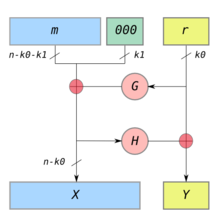
\includegraphics[scale=0.8]{Cattura27.png} 
\end{tabular}\\\\
This scheme is also called \textbf{All-Or-Nothing security}, in fact, in order to retrive $m$ we must have $X$ and $Y$, since we need $X$ in order to retrieve $r$ from $Y$ and we need $r$ in order to retrieve $m$ from $X$. 
\subsubsection{El Gamal Encryption}
\textbf{El Gamal} it's a mode of \emph{encryption} strongly based on \emph{Diffie-Hellman key exchange approach}, indeed we will see that the underlying math is the same.\emph{ El Gamal }is an alternative to \emph{RSA} and so is able to generate a \emph{pair of keys public/private}, in order to perform \textbf{encryption} and \textbf{decryption}. The protocol is the following: given a \emph{prime} $p$ and a \emph{generator} of the $Z_p$ \emph{cyclic group} of order $p$, \emph{Alice} chooses an $x$ in the range $\left [1,p-1 \right]$ as the \textbf{private key}, and she chooses the number $g^x \; mod\; p$ as the \textbf{public key}. If \emph{Bob} wants to send a \emph{message} $m \in Z_p$ to \emph{Alice}, he chooses a number $y$ in the range $\left [1,p-1 \right]$ and he sends to \emph{Alice} the pair: $(g^y \; mod\; p, m\cdot g^{xy} \; mod\; p)$. He can send the second \emph{message} cause he knows $m,y$ and $g^x \; mod\; p$ which is the \emph{public key} of Alice. When \emph{Alice} gets the \emph{pair} of \emph{messages}, she uses the first one in order to compute $g^{xy} \; mod\;  p$ then she finds a number $(g^{xy})^{-1} \; mod\; p$ and so she can get the \emph{message} as follows: $m = m \cdot g^{xy} \cdot (g^{xy})^{-1} \; mod\; p = m \; mod\; p = m$. This scheme requires two \emph{exponentiations} per each \emph{transmitted block}, so it require a little bit demanding in terms of \emph{computational effort}. 
\section{Digital Signature - DSA}
A \textbf{Digital signature} is a mathematical scheme for demonstrating the \textbf{authenticity} of \emph{digital messages} or \emph{documents}. A valid \emph{digital signature} gives a recipient reason to believe that the \emph{message} was created by a \emph{known sender} (\textbf{authentication}), that the \emph{sender} cannot deny having sent the \emph{message} (\textbf{non-repudiation}), and that the \emph{message} was not altered in transit (\textbf{integrity}). In few words, a \emph{digital signature} provides \emph{authentication}, \emph{integrity} and \emph{non-repudiation}. We already studied an approach for \emph{data integrity}, it was based on \emph{MACs}. Let's suppose that Alice and Bob share a secret key K, then $(M,MAC_K(M))$ will convince Alice that the message was created by Bob. But in case of dispute A cannot convince a judge that $(M,MAC_K(M))$ was sent by Bob, since A could generate it herself. \\\\
Then we discussed \emph{RSA} and in general about the usage of \textbf{public and private keys}:
\begin{itemize}
\item \textbf{Encryption with other party’s public key}: you get \textbf{confidentiality} (he \emph{decrypts} with his \emph{private key});
\item \textbf{Encryption with my private key}:\textbf{ no confidentiality}, but \textbf{authentication} (everyone is enabled to \emph{decrypt} my \emph{ciphertext}, it is just sufficient to use my \emph{public key} in order to do it, but in this way other \emph{parties} can be sure about the fact that it was me who \emph{encrypted} the \emph{message});
\end{itemize}
So, it's easy to \textbf{forge signatures} of \emph{random message} even without holding $D_A$, in fact \emph{Bob} can pick an $R$ arbitrarily and can compute $S=E_A(R)$, this means that the pair $(S,R)$ is a \textbf{valid signature} of \emph{Alice} (even if it was created by \emph{Bob}), so the scheme is subject to \textbf{Existential Forgery}, that is the ability of an \emph{adversary} to create a \emph{pair}, \emph{message} and \emph{signature}, where the \emph{message} has not been signed in the past by the \emph{legitimate signer} but the \emph{adversary} doesn't have any control over the \emph{message}. In the \textbf{Selective Forgery} instead, the \emph{adversary} creates a pair \emph{message signature}, where the \emph{message} has been chosen by the \emph{adversary} prior to the \emph{attack}, if an \emph{adversary} can do the \emph{selective forgery} it can also do the \emph{existential forgery}. In the \textbf{Universal Forgery} instead an \emph{adversary} can create a \emph{valid signature} for any given \emph{message}, and this is the strongest ability in \emph{forging} and it implies all the other types of \emph{forgery}. So we need a method to prevent the \emph{Existential Forgery} and this method is the \textbf{hashing}. \\\\
An \emph{adversary} can use the \textbf{forgery attack}, in fact he can generate a \emph{random file} $T$ and will \emph{encrypt} it with the $K_p$ (\emph{public key of Bob}). The \emph{ciphertext} generated will be $R= E_{K_p}(T)$ then the \emph{attacker} sends $R$ as \emph{plaintext} and $T$ as \emph{digital signature}. \emph{Alice} will take the \emph{digital signature} $T$ and so she \emph{encrypts} $T$ with $K_p$ of \emph{Bob} and she gets $E_{K_p}(T) = R$, but since the \emph{attacker} sent $R$ as \emph{plaintext}, \emph{Alice} sees that the \emph{decryption} of the \emph{digital signature} matches with the \emph{plaintext} sent, so she accepts the \emph{document}. That’s why all this is not good.\\\\
Let $E_A$ be \emph{Alice} \emph{public encryption key}, and $D_A$ the \emph{private decryption key}: 
\begin{itemize}
\item In order to \textbf{sign} the \emph{message} $M$, \emph{Alice} will compute two \emph{strings}: $y=H(M)$ and $z=D_A(y)$ and then will send to \emph{Bob} $(M,z)$;
\item In order to \textbf{verify} the \emph{Alice's signature}, \emph{Bob} will compute the \emph{string} $y= E_A(z)$ and will check if $y=H(M)$;
\end{itemize}
\emph{Alice} create $z$ with $D_A$ (the \emph{decrypt function}) cause it need to use it's \textbf{private key} to \emph{encrypt} it, instead \emph{Bob} will read $y$ using $E_A$ (the \emph{encrypt function}) to \emph{decrypt} it with the \textbf{public key} of \emph{Alice}. The function $H$ should be \textbf{collision resistant} so that cannot find another $M^{'}$ with $H(M) = H(M^{'})$. With \textbf{hashing} the process of \emph{signing} is much faster, we are using \emph{asymmetric encryption}, which is slow, but here it is performed on the \emph{hash} of the document which is much smaller than the \emph{plain document}. 
\subsection{Standards for Digital Signatures}
The structure of the \emph{general digital signature} is divided in three steps, the \textbf{generation} of \emph{private and public keys} (in a \emph{random} way), the \textbf{signing} (\emph{deterministic} or \emph{randomized}), and the \textbf{verification} (\emph{accept} or \emph{refuse}) usually \emph{deterministic}. There are three different schemes used in practice: \textbf{RSA}, \textbf{El Gamal} and the \textbf{DSS}.
\subsubsection{RSA and PKCS\#1}
We already saw the \textbf{PKCS\#1 standard}, the \emph{signature} is made by \emph{hashing} using the \emph{private key}, only the person who knows the \emph{secret key} can \emph{sign}, everybody can verify the \emph{signature} by using the \emph{public key}. We construct the \emph{digital signature} by \emph{encrypting} with our \emph{private key} the following \emph{message}:
\[ 0 \parallel 1 \parallel at\; least\; 8\; byte\; FF\; base\; 16 \parallel 0 \parallel specs\; of\; hash\; function \parallel hash(M)\]
Where:
\begin{itemize}
\item The first byte $0$ ensures that the \emph{message} is less than $N$;
\item The second byte $1$ denotes \emph{signature}, if it's $2$ it means that the \emph{message} is \emph{encrypted} for \emph{confidentiality} purpose;
\item The bytes $1111111.....$ implies that the \emph{encoded message} is large;
\item And $M$ is the \emph{original message};
\end{itemize}
As a conclusion for \textbf{RSA} I want to stress the concept that when you are using \emph{RSA} you want to \emph{sign}, the other typical usage of \emph{RSA} is send an \textbf{encrypted key}. You don’t use \emph{RSA} for \emph{confidentiality} purpose, for \emph{encrypt} a \emph{document}, you \emph{encrypt} just a \emph{key}. Because of its \emph{complexity}, \emph{computational effort,} much bigger than Rijndael. PKCS\#1 define a \textbf{Signature Scheme with Appending} or \textbf{SSA}, in which the \emph{appendix} is the \emph{signature} added to the \emph{message}, and we don't consider \emph{signature schemes} with \emph{message recovery} (\emph{message} is embedded in the \emph{signature}). There are two approaches that differ in how the \textbf{encoded message} is obtained:
\begin{itemize}
\item \textbf{RSASSA-PSS}: a \emph{probabilistic signature scheme} that uses \textbf{EMSA-PSS} an \emph{encoding method} for \emph{signature appendix}, inspired to \emph{OAEP} that makes use of \emph{random salt} added per \emph{signature}, in which first the message is hashed, after the output is padded and we add a salt at the end so we generate a new message, and this message will be hashed and then XORed with another padding and salt that will be concatenated to $h(M)$;
\item \textbf{RSASSA-PKCS1-v1.5}: that is \emph{deterministic};
\end{itemize}
\subsubsection{El-Gamal Signature Scheme}
\textbf{El-Gamal scheme} can be divided into three parts: \emph{generation}, \emph{signing} and \emph{verification}. The \textbf{generation} of the \emph{key} is made as:
\begin{itemize}
\item Choose a \emph{prime} number $p$ of 1024 bits such that the \textbf{Discrete Logarithm} \textbf{(DL)} in $Z_p^{*}$ is \emph{hard}, the only way to get the \emph{private key} $x$ is by computing the \emph{discrete logarithm} of $p$ in base $g$; 
\item Find a \textbf{generator} $g$ og $Z_p^{*}$, an integer for which the \emph{powers} are congruent with the numbers \emph{coprime} with $p$; 
\item We pick a $x$ in $\left [ 2 , p-2 \right ]$ at random;
\item Compute $y= g^x \; mod\; p$; 
\item Then the public key $K_p = (p,g,y)$ and the private key $K_s = x$;
\end{itemize}
In order to \textbf{generate} the \emph{signature} instead, if we want to sign a \emph{message} $M$ we define a new pair of \emph{keys} $(r,k)$, where $r$ is a \emph{public key} instead $k$ is a \emph{private key} used in order to have a different \emph{signature} every time:
\begin{itemize}
\item We will start by compute the \emph{digest} $m = H(M)$;
\item We will pick $k$ in $\left[ 1, p-2 \right]$ coprime to $p-1$ at random;
\item After we will compute $r = g^k\; mod \; p$ and $s = (m-rx)k^{-1} \; mod\; (p-1)$, if $s$ is 0 then we need to restart; 
\item The \emph{output signature} will be $(r,s)$;
\end{itemize}
The \textbf{verification} follows this pattern:
\begin{itemize}
\item First we compute $m=H(M)$;
\item We will accept only if $0<r<p \wedge 0<s<p-1 \wedge (y^r \cdot r^s = g^m)\; mod\; p$;
\item Since we have that $s = (m-rx)k^{-1} \; mod\; (p-1)$ we have that $sk +rx = m$ (\emph{mod(p-1) disappears cause mistero della fede}). Now:
\begin{itemize}
\item We know that $r=g^k\; mod\; p$ so if we power left and right operands for $s$ we obtain: $r^s = g^{ks} \; mod	\; p$;
\item We know that $y=g^x\; mod\; p$ so if we power left and right operands for $r$ we obtain: $y^r = g^{rx}\; mod	\; p$ ;
\item If we multiply we obtain: $y^r \cdot r^s = g^{ks + xr} \; mod	\; = g^m \; mod\; p$;
\end{itemize}
\end{itemize}
\subsection{DSS, Digital Signature Standard}
\textbf{DSS} is important because is the choice made by \emph{NIST}, it is inspired on \emph{El-Gamal approach} and according to the original formulation \emph{DSS} is using \emph{SHA}, just because the \emph{hashing function} chosen by the \emph{NIST} is \emph{SHA}. There are two acronyms: \textbf{DSS}, \textbf{Digital Signature Standard} and \textbf{DSA} , \textbf{Digital Signature Algorithm}. The second is just an \emph{algorithm} in order to get the \emph{digital signature}. \\\\
The idea of \textbf{DSA} is to use two prime numbers $p$ and $q$ such that:
\begin{itemize}
\item $p$ is a $L$ bit prime number such that the Discrete Log problem \emph{mod p} is intractable;
\item $q$ is a 160 bit prime that divides $p-1$, so we have that $p = j \cdot q +1$, so $j$ is a constant equal to $j = \frac{p-1}{q}$; 
\end{itemize}
Then let $\alpha$ be a $q^{th}$ root of $1\; mod\; p$, so we have that $\alpha^q = 1\; mod\; p$. In order to compute $\alpha$ we need to take a random number $h$ such that $1< h < p-1$ and we compute $g=h^{\frac{p-1}{q}}\; mod\; p = h^j\; mod \; p$, since we need to apply the \emph{little theorem of Fermat}, we need that $h$ is \emph{coprime} with $p$. If $g=1$ we have to choose a different $h$ for \emph{security reason}. Then it holds that $g^q = h^{p-1} = 1\; mod\; p$ by the \textbf{Fermat Theorem}, since $p$ is prime and every number less than $p$ raised to $p-1$ are equal to $1\; mod\; p$. Finally we choose $\alpha = g$. \\\\ 
\textbf{Math proof}: $g= h^j\; mod\; p = h^{\frac{p-1}{q}}  \; mod\; p$ so if we power both the operators with $q$ we have: $g^q = h^{p-1} \; mod\; p$ and that from the Fermat Theorem $g^q = (1 \; mod\; p) \; mod\; p$ so we obtain that $g^q = 1 \; mod\; p = \alpha^q$. \\\\
So now let's talk about the algorithm, we have to choose two prime numbers $p,q$ such that $p-1 = 0\; mod\; q$ (so $p-1$ is a multiple of $q$) and we consider $\alpha$ as the $q^{th}$ root of $1\; mod\; p$. Then the \textbf{private key} will be $s$ a random integer $1 \leq s \leq q-1$ and the \textbf{public key}: $(p,q,\alpha,y = \alpha^s \; mod \; p)$. $s$ will be hard to find since an \emph{adversary} should compute the \emph{discrete log}, and choosing a $t$ that computing the discrete log of $mod\; p$ of the multiplicative group $Z_p^{*}$ is hard. The \emph{signature} is inspired to \emph{El-Gamal}, in fact we choose a random integer \emph{secret} in the range $\left[1,q-1 \right]$ and we have two parts:
\begin{itemize}
\item Part 1: $P_1= (\alpha^k\; mod\; p)\; mod\; q$;
\item Part 2: $P_2=(SHA(M)+ s \cdot P_1) \cdot k^{-1}\; mod\; q$;
\end{itemize}
Also the \textbf{verification} is done in two parts: 
\begin{itemize}
\item $e_1 = SHA(M) (P_2)^{-1} \; mod \; q$;
\item $e_2 = P_1 \cdot (P_2)^{-1} \; mod\; q$; 
\end{itemize}
And the \emph{signature} will be accepted only if $(\alpha^{e_1} \cdot y^{e_2} \; mod\; p) \; mod\; q = P_1$. The \emph{proof} of the \emph{correctness} of this is:
\begin{figure}[H]
  \centering
  \includegraphics[scale=0.5]{cattura28.png}
\end{figure}
So, starting from the \emph{Part 2}, we isolate the $k\; mod\; q$, after from the definition of the $y$ and from the \emph{verify formula} we obtain $\alpha^{e_1}(\alpha^{s\cdot e_2}\; mod\; p)\; mod\; p$ that we can rewrite as $\alpha^{e_1 + s \cdot e_2} \;mod \; p$. Now we will use the formula obtained before and we get $\alpha^{k\; mod\; q}\; mod\; p$ that is equal to $\alpha^{k}\; mod\; p$ cause $k$ is a value less than $q$. Note that the external $mod\; q$ there was since the beginning of the proof but we omitted it. At the end: $(\alpha^{e_1} \cdot y^{e_2}\; mod\; p)\; mod\; q = (\alpha^k \; mod\; p) \; mod\; q = P_1$.
\\\\\
The \textbf{security of DSS} is \emph{ensured} cause the \emph{secret key} $s$ is not \emph{revealed} and it cannot be \emph{forged} without knowing it, and we use a \emph{random number} for \emph{signing} ($k$) that is not \emph{revealed}, and we don't have any \emph{duplicates} of the same \emph{signature} even with the same \emph{message}. It's important to note that if $k$ is known then you can compute $s\; mod\; q = s$, since $s$ is less than $q$, and that we have two \emph{signed messages} with the same $k$ then $k$ value can be \emph{reveled}, so combined with the precedent equation it's possible to find $s$. \\\\
Finding two \emph{primes} $p$ and $q$ such that $p-1 = 0\; mod\; q$ it's \textbf{not easy} and can take time, and $p$ and $q$ are \emph{public} so they can be used by \emph{many persons}. So, we have that \emph{DSS} is faster than \emph{RSA} for \emph{signing} if we have some \emph{preprocessing}, but the problem is to generate \emph{random numbers} that may depend on the \emph{message} so in this case we can't have \emph{preprocessing}. \emph{RSA} is usually used for \emph{signature} and for \emph{key management}. \\\\
When a \emph{document} needs to be \emph{signed} in many cases it's important for a formal point of view that also the the \textbf{time} is certified. This is called \textbf{Timestamping}, so we associate a \emph{timestamp} to a \emph{document}, in many cases we use a \emph{third party} (an \emph{authority}) also called \textbf{TSA} (\textbf{TimeStamping Authority}), who signs the \emph{document} with the \emph{timestamp}. If \emph{Alice} want to \emph{timestamp} a \emph{document}:
\begin{itemize}
\item \emph{Alice} compute \emph{hash} of \emph{document} and sends it to \emph{TSA}; 
\item \emph{TSA} will add the \emph{timestamp}, will compute a new \emph{hash} (of \emph{timestamp} and \emph{received hash}) and will \emph{sign} the obtained \emph{hash} and after will reply to \emph{Alice};
\item \emph{Alice} will keep the \emph{TSA signature} as a proof, so everybody can check the \emph{signature}, and \emph{TSA} doesn't know \emph{Alice's} \emph{document}; 
\end{itemize}
\section{Authentication}
\textbf{Authentication} is the procedure of providing the \textbf{identity} to a \emph{party} in order to \emph{access services} that this \emph{party} provides to the \emph{allowed ones}, in our example \emph{Alice} needs to show her \emph{identity} to \emph{Bob}, cause \emph{Bob} wants to show \emph{information} only to \emph{authorized people}. One of the most common \emph{attacks} against \emph{authentication} is \textbf{Spoofing}, that is the ability to cheat about the \emph{identity} of the creator of the \emph{message}, in fact with \emph{authentication} we want to prevent \emph{spoofing attacks}. We have two interesting cases of \emph{authentication}:
\begin{itemize}
\item A \emph{computer} is authenticating another \emph{computer}; 
\item A \emph{person} is using a \emph{public workstation}, so we don't want to store \emph{secrets} for all the possible \emph{user};
\end{itemize}
The \textbf{Closed World} assumption, it's an idea based on the sentence: \textbf{what is not currently known to be true, is false}. So it basically means that everything is \emph{false} until we can prove that it's \emph{true}. Many people don’t like it because they prefers the concept of\emph{ black list} (forbidden or bad things) and \emph{white list} (allowed things). Your \emph{environment} is considered a \textbf{Closed Environment} when you are working in a \emph{closed place}, like your enterprise. In many cases you are somewhat \emph{dealing} with a \textbf{third-party} (a \textbf{trusted server}) that is protected by many methods, this \emph{server} can support \emph{authentication} of many \emph{users}, we will see \emph{Kerberos} that is a very \emph{secure environment}. If the \emph{attacker} belongs to the same company, it is called an \textbf{insider}, and it has a lot of power compared to an \emph{external one}. \\\\
There are many differences between \textbf{authenticating a human and a computer}. 
\begin{itemize}
\item \textbf{Computers} can store a \emph{high-quality secret}, such as a \emph{long random-looking number} (\emph{key}), and they can do \emph{cryptographic operations};
\item \textbf{Humans} instead are not able to do this, they use some \emph{passwords} that are very different from a \emph{key};
\end{itemize}
The first difference between a \emph{password} and a \emph{key}, is that \emph{humans} are stupid, so they use \emph{password} that contains \emph{words}, and \emph{words} belongs to a \emph{dictionary}, so an \emph{adversary} can run an attack called \textbf{Dictionary Attack}, a \emph{probabilistic attack} that use most common \emph{words} in order to find a \emph{password}. Also \emph{password} are usually \emph{short} and \emph{easy to be guessed} by an \emph{attacker}. Instead \emph{computers} stores \textbf{long keys}, usually \emph{hidden} or \emph{encrypted} or also \emph{one-time password}. One of the most common \emph{attack} is the \textbf{Login Trojan Horse}, in which an \emph{attacker} prompts a \emph{fake login window} that induces the innocent user to prompt the \emph{password} that is collected by the \emph{attacker}. \\\\
The \textbf{authentication of people} can be based on \emph{password}, \emph{smart card}, \emph{biometric tools} or \emph{network address}. \emph{Biometrics} are usually used, like \emph{retina examination}, \emph{fingeprinting reader} or \emph{voice}, but we can have \emph{false positive} and \emph{false negative} (like \emph{fake fingerprints}, or \emph{modified voices}).  \\\\
There are three main approaches in order to achieve \textbf{authentication} and they are:
\begin{itemize}
\item \textbf{Shared secret key}: \emph{Alice} and \emph{Bob} share a \emph{secret key} and use it to \emph{authenticate} each other;
\item \textbf{Authentication through a Third Party}: there is an \emph{external server} and if two \emph{users} want to authenticate each other they have to pass through the \emph{server};
\item \textbf{Public Key Criptography}: users use the \emph{Public Key Infrastructure} in order to achieve \emph{authentication};
\end{itemize}
We can use different \emph{techniques} in order to \emph{authenticate} an \emph{user} through a \emph{key}, like \textbf{Timestamp}, or a \textbf{Nonce}, a random number chosen by the \emph{user} that \emph{authenticates} to verify the other knows the \emph{key}, or \textbf{Sequence Numbers}, like in \emph{TCP} that uses \emph{sequence numbers} in order to do some things like tracking the order of \emph{connections}. It's very important that we need to guarantee \emph{authentication} and \emph{integrity} that \textbf{Encryption doesn't guarantee Authenticity of a message}. 
\subsection{Authentication by Symmetric Key}
We denote with $K_{AB}$ the \emph{secret key} shared between $A$ and $B$, and with $K\{M\}$ we denote that $M$ is \emph{encrypted} with the \emph{secret key} $K$, with $R$ we denote the \emph{Nonce}, but the challenge can be called $R$ or $K_{AB}$. There are several ways to obtain \textbf{authentication} through \textbf{symmetric keys:}
\begin{itemize}
\item \textbf{One Way authentication using Nonce (Challenge)};
\item \textbf{One Way authentication using Timestamps};
\item \textbf{Two Ways (mutual) authentication using Nonce};
\end{itemize}
\subsubsection{Challenge/Response Authentication}
\begin{tabular}{C{10cm}  L{10.5cm}}
\emph{Alice} want to \textbf{authenticate} \emph{Bob}, she will send to him a \emph{plaintext}, presenting herself, \emph{Bob} will respond with a \textbf{challenge} (that is $R$, the \emph{nonce}), then \emph{Alice} will reply with the \emph{encrypted version} of $R$ with the \emph{key} $K_{AB}\{R\}$ (the correct answer of the \emph{challenge}). If \emph{Bob} receives the right \emph{encryption} then he authenticate \emph{Alice}. This scheme is \textbf{not mutual} (in fact \emph{Bob} authenticates \emph{Alice}, but \emph{Alice} doesn't). This scheme can be \emph{easily attacked}, cause \emph{Alice} cannot be sure that she is \emph{authenticating} actually to \emph{Bob}, so maybe she talking with the \emph{attacker} (\emph{Trudy}) that is able to send a \emph{challenge} $R$ and will get $K_{AB}$ that can be derived from a \textbf{password} that \emph{Trudy} can try to obtaining from $R$ and $K_{AB}$. & \includegraphics[scale=0.55]{cattura29.png}
\end{tabular}
\hfill \break
\\
\begin{tabular}{C{10cm}  L{10.5cm}}
There is \textbf{variant} in which \emph{Alice} again start presenting herself, but now the \emph{challenge} sent by \emph{Bob} is the encrypted $R$ and then \emph{Alice} is expected to find the \emph{nonce} $R$, then she sends $R$ to \emph{Bob} in order to be \emph{authenticated}. This \emph{variant} provides a little bit more \emph{security}, because when \emph{Bob} sends the \emph{challenge}, we understand that only \emph{Bob} can generate that \emph{challenge} (only him knows the \textbf{private shared key}), so \emph{Alice} can be sure it is \emph{Bob} that is sending the \emph{challenge}. So \emph{Alice} can trust the \emph{party} with who she is \emph{authenticating}. This doesn't change a lot for the adversary cause he still can obtain $R$ and $K_{AB}$. If $R$ has a \textbf{limited lifetime}, like \emph{random numbers} plus \emph{timestamp}, meaning that we can consider it valid for a small amount of time after which it is not valid anymore, then \emph{Alice} trusts \emph{Bob}, because the limited lifetime of $R$ does not allow \textbf{replay attacks}. & \includegraphics[scale=0.55]{cattura30.png}
\end{tabular}
\subsubsection{Timestamp Authentication}
\begin{tabular}{C{9cm}  L{10.5cm}}
In which \emph{Alice} and \emph{Bob} have \textbf{reasonably synchronized clock} (this can be a weakness). \emph{Alice} sends to \emph{Bob} the \emph{encrypted timestamp}, then if \emph{Bob} can \emph{decrypt} he can authenticate \emph{Alice}, the \emph{timestamp} has a \emph{timeout} after which it expires, therefore if \emph{Bob} saves that \emph{timestamp} until expires, no \emph{replay attack} is possible. It is very efficient in fact there are no \emph{intermediate states} like before. 
 & \includegraphics[scale=0.55]{cattura31.png}
\end{tabular}
\subsubsection{Mutual Authentication}
\begin{tabular}{C{11cm}  L{10.5cm}}
In the \textbf{Mutual Authentication} as the \emph{one-way authentication}, \emph{Alice} presents to \emph{Bob}, and \emph{Bob} reply with the \emph{nonce} $R_1$, and \emph{Alice} responds with the \emph{encrypted version} of $R_1$. Now \emph{Alice} is challenging \emph{Bob} so she sends him the \emph{nonce} $R_2$ and \emph{Bob} sends back the \emph{encrypted} $R_2$. But we have too many \emph{messages}. 
& \includegraphics[scale=0.55]{cattura32.png}
\end{tabular}
\hfill \break
\\
\begin{tabular}{C{11cm}  L{10.5cm}}
This \textbf{variant} is a compact way to do the \emph{mutual authentication}, \emph{Alice} presents to \emph{Bob}, together with the \emph{challenge} $R_2$, \emph{Bob} replies with his \emph{challenge} $R_1$ and with the response to \emph{Alice's challenge}. Finally \emph{Alice} sends back the response to \emph{Bob's challenge}. In this way we only exchange 3 \emph{messages}, but this variant suffer the \textbf{Reflection Attack}.
& \includegraphics[scale=0.55]{cattura33.png}
\end{tabular}
\hfill \break
\\
\begin{tabular}{C{11cm}  L{10.5cm}}
The \textbf{Reflection Attack}, is an \emph{attack} that aims to \emph{construct} an extra \emph{session} useful just for the \emph{adversary}. The \emph{second session} will be left \emph{uncompleted}, but is used by the \emph{attacker} to complete the first one. \emph{Trudy} is pretending to be \emph{Alice} (\emph{messages} are \textbf{spoofed}), so she sends to \emph{Bob} “\emph{I’m Alice, this is my challenge} $R_2$”, \emph{Bob} is correcting responding with \emph{encrypted} $R_2$, but \emph{Trudy} cannot send back the \emph{encrypted} $R_1$ cause it doesn't know the \emph{key}. So she start another \emph{session} with \emph{Bob} with the \emph{challenge} $R_1$ that received from \emph{Bob} in the \emph{first session}, and in the \emph{second session} he will get the \emph{correct result} of the \emph{encryption} of $R_1$ with another \emph{challenge} $R_3$, that he will \emph{ignore}. \emph{Bob} can obviously suspect because the \emph{second session} will be uncompleted. We can have two different solutions, like using \emph{different keys} for each \emph{session} ($K_{AB}$ and $K_{AB}+1$) or \emph{different challenges}.
& \includegraphics[scale=0.55]{cattura34.png}
\end{tabular}
\hfill \break
\\
\begin{tabular}{C{11cm}  L{10.5cm}}
This is another \textbf{variant less optimized}, in which the number of \emph{messages} exchanges is 4. \emph{Trudy} can set up an \textbf{offline-password attack}, so she plays as \emph{Bob}, she sends the \emph{challenge} and \emph{Alice} sends her back the \emph{correct response}, so \emph{Trudy} by knowing the \emph{pair} $(challenge,response)$ can guess the \textbf{secret key} with brute force.& \includegraphics[scale=0.45]{cattura35.png}
\end{tabular}
\clearpage
\subsection{Authentication trough Third-Party}
Since each \emph{user} must have a \emph{different key} for every other \emph{user}, we have a \emph{quadratic} number of \emph{keys}, and this is a problem. For this reason we will use a \textbf{Trusted Party} that realizes the \emph{authentication}. It is a very typical scenario used by companies and enterprises, and this \emph{third party} is called \textbf{Key Distribution Center} (\textbf{KDC}), or \textbf{Authentication Server}, usually we denote it with $C$. Every \emph{participant} in the \emph{network} is sharing a \emph{secret key} only with this \emph{server}, so with $n$ parties there are $n$ \emph{secret keys} that the \emph{server} maintains and this means that every \emph{user}, every \emph{party} has to be registered to the \emph{server}. Now having this \emph{server}, we want to implement \emph{single} or \emph{mutual authentication} as before. An optional would be to use a \textbf{session key} for \emph{short time communications}. If the \emph{attacker} is an \textbf{insider}, he is sharing a \emph{private key} with the \emph{server}, he can \emph{sniff} and spoof\emph{ messages}, but he cannot guess \emph{random numbers} generated by the \emph{parties} and cannot be able to get the \emph{private keys} of other \emph{parties} and cannot \emph{decrypt messages} in short time without knowing the \emph{key} because the \emph{attacker} is expected not to have high \emph{computational power}. 
\subsubsection{First schema}
\begin{tabular}{C{11cm}  L{10.5cm}}
The \textbf{first schema} is presented just for educational purposes, in fact it's \textbf{very simple} and \textbf{weak}. \emph{Alice} wants to talk with \emph{Bob}, so she sends a message to $C: A,B$, saying \emph{I am Alice, I want to talk with Bob}, $C$ chooses the \textbf{session key $K$ }and sends \emph{Alice} two \emph{messages} that are $K$ \emph{encrypted} with $K_{AC}$ and $K$ encrypted with $K_{BC}$. \emph{Alice} will \emph{decode} and will compute $K$, and will send to \emph{Bob} a message constituted by three elements $(C,A,K_{BC}(K))$ like ''\emph{I’m Alice, I obtained this thing by }$C$, \emph{this thing is }$K_{BC}(K)$”. So Bob can decrypt $K_{BC}(K)$ and will find $K$ and will reply to \emph{Alice}, a \emph{message} encrypted with the \emph{session key}: $K$(''\emph{Hello Alice this is Bob}'').
& \includegraphics[scale=0.65]{cattura36.png}
\end{tabular}
\hfill \break \\
\begin{tabular}{C{11cm}  L{10.5cm}}
This \emph{schema} can be \textbf{attacked} in fact, if we assume that \emph{Trudy} can \textbf{sniff} and \textbf{spoof} then she can make the \textbf{Man In The Middle Attack}, with \emph{Trudy} between them, so she can intercept \emph{messages}, and create a \emph{session key} between her and \emph{Alice}, and another between her and \emph{Bob}. \emph{Alice} sends to \emph{Trudy} (instead of $C$): $A, B$ (\emph{I am Alice, I want to talk with Bob}). Immediately \emph{Trudy} sends to $C$: $A,T$ (\emph{I am Alice, i want to talk with Trudy}), so $C$ will choose a $K$ and will send to Alice: $(K_{AC}(C),K_{TC}(C))$. When \emph{Alice} sends to \emph{Bob} the \emph{message} of three elements: $C, A, T_{TC}(K)$ \emph{Trudy} will intercepts it and will reply to \emph{Alice} with the \emph{session key}: $K$(''\emph{Hello Alice this is Bob}''). & \includegraphics[scale=0.65]{cattura37.png}
\end{tabular}
\begin{tabular}{C{11cm}  L{10.5cm}}
In order to \emph{solve} this \textbf{problem} we can modify the \emph{protocol} in such a way that when \emph{Alice} wants to talk with \emph{Bob}, she send to $C: A, K_{AC}(B)$ so the \emph{receiver} is \textbf{encrypted}, so an \emph{attacker Trudy} cannot know that \emph{Alice} wants to talk with \emph{Bob}.  
& \includegraphics[scale=0.6]{cattura38.png}
\end{tabular}
\hfill \break \\ 
\begin{tabular}{C{11cm}  L{10.5cm}}
Even this scheme is \emph{violable}, in fact if Alice want to talk with \emph{Bob} like before $A,K_{AC}(B)$, but in precedence \emph{Trudy} and \emph{Alice} had already talk, \emph{Trudy} can use these \textbf{previously exchanged messages}, and will intercept the \emph{message} of $A$, and will send to $C: A,K_{AC}(T)$, even if \emph{Trudy} doesn't know with who \emph{Alice} wants to talk. $C$ will choose a $K$ and will send to Alice: $K_{AC}(K), K_{TC}(K)$. Now \emph{Alice} will \emph{decode} $K$ and will send to $B$ the message of three elements: $C, A, K_{TC}(B)$, \emph{Trudy} will get it and finds that \emph{Alice} want to talk with \emph{Bob}, so she will now acts in place of \emph{Bob}.
& \includegraphics[scale=0.6]{cattura39.png}
\end{tabular}
\subsubsection{Needham-Schroeder Protocol}
The \textbf{Needham-Schroeder Protocol} it's a very important \emph{protocol} that poses the basis for \textbf{Kerberos} and it's used to create a \emph{session key} between two \emph{parties} by means of a \emph{third party} and it's based on \emph{Nonce} and \emph{challenge response}. If \emph{Alice} wants to talk with \emph{Bob}, she chooses a \emph{Nonce} $N$ and will send to $C$: $A,B,N$. When $C$ receives the \emph{request}, will generate a \emph{session key} $K$, and replies to \emph{Alice} an \emph{encrypted message} by means of the \emph{secret key} of \emph{Alice} $K_{AC}(N,K,B,K_{BC}(K,A))$, the \emph{message} contains the \emph{nonce}, the \emph{session key}, the identity of \emph{Bob}, and the \emph{encryption} of $K$ and $A$ by means of the \emph{key} of \emph{Bob}. \emph{Alice} will \emph{decodes} the \emph{message}, will check $N$ and $B$, and will send to \emph{Bob}: $K_{BC}(K,A)$. \emph{Bob} will \emph{decode} this \emph{message}, will choose another \emph{Nonce} $N^{'}$ and sends back to \emph{Alice}: $K($\emph{This is Bob,}$N^{'}$). \emph{Alice} can reply with a \emph{message encrypted}: $K($\emph{This is Alice},$N^{'}-1)$ so \emph{Alice} replies with the \emph{nonce} decremented by one. It's important to note that \emph{Bob} is not communicating with $C$. Also this \emph{protocol} can be \emph{attacked}, and this is called \textbf{Denning \& Sacco Attack}, it works as a \emph{replay attack} and uses an old session key. Like before \emph{Alice} chooses a $N$ and sends to $C$: $A,B,N$, then $C$ chooses $K$ and sends to $A$: $K_{AC}(N,K,B,K_{BC}(K,A))$ but now \emph{Trudy} will acts in place of \emph{Alice}. \emph{Alice} will \emph{decode} and check $N$ and $B$ and will send to \emph{Bob} $K_{BC}(K,A)$. \emph{Trudy} as \emph{Alice} replays to Bob $K_{BC}(K^{'},A)$, with $K^{'}$ an \textbf{older session key}. \emph{Bob} will \emph{decode}, will choose an $N^{'}$ but will send to \emph{Trudy} instead of Alice $K^{'}($\emph{This is Bob,}$N^{'}$). So Trudy will reply to Bob: $K^{'}($\emph{This is Alice},$N^{'}-1)$. \\\\
We can also have \emph{Trudy} that uses the \emph{Man in the Middle Attack}, if we have a \emph{session key} that is compromised. There are many possible variants of this \emph{attack}, and all these \emph{variants} are important just to let us understanding why we need to introduce more ingredients like \textbf{timestamps}, \textbf{sequence numbers} and so on. Therefore a \emph{variant} of the \emph{protocol} has been invented:
\subsubsection{Needham-Schroeder Protocol variant}
Since the \emph{original protocol} was \emph{weak} and we have seen some attacks against it, the \emph{protocol} has been \textbf{revisited} and here is the new version:
\begin{itemize}
\item $C$ exchanges \emph{messages} with both $A$ and $B$;
\item \emph{Timestamp} $t$ is used only between $B$ and $C$;
\item $K$ \emph{session secret key};
\end{itemize}
\begin{enumerate}
\item \emph{Alice} chooses a \emph{nonce} $N$ and sends to \emph{Bob}: $(A,N)$;
\item \emph{Bob} chooses a \emph{nonce} $N^{'}$ and sends to the \emph{Server} $(B,N^{'}, K_{BC}(N,A,t))$;
\item The \emph{Server} sends to \emph{Alice}: $(K_{AC}(B,N,K,t), K_{BC}(A,K,t), N^{'})$;
\item \emph{Alice} sends to \emph{Bob}: $(K_{BC}(A,K,t), K(N^{'}))$;
\end{enumerate}
So in few words, \emph{Alice} wants to talk to \emph{Bob}, so she sends him a \emph{nonce} $N$. \emph{Bob} sees this \emph{message} and create a \emph{nonce} $N^{'}$ and a \emph{timestamp} $t$ and sends to the \emph{Server} the \emph{encrypted version} by means of $K_{AC}$ of the two elements, so only \emph{Bob} and the \emph{Server} knows the \emph{timestamp}, and the \emph{Server} will have the power to say if the \emph{timestamp} is valid or not. Then the \emph{Server} sends to \emph{Alice} the \emph{encrypted session key} and the \emph{encrypted timestamp} by means of $K_{AC}$, and another \emph{encrypted message} by means of $K_{BC}$ that \emph{Alice} has to forward to \emph{Bob}, with the \emph{nonce} of \emph{Bob encrypted} with the new \emph{session key}. 
\subsubsection{Needham-Schroeder Protocol Expanded}
\emph{Alice} want to talk with \emph{Bob}, \emph{Bob} generate a \emph{nonce} and sends it to \emph{Alice} encrypted by the \emph{secret key} of \emph{Bob}, now \emph{Alice} sends a \emph{message} to the \emph{Server}. Then the \emph{Server} generates the \emph{session key} $K_{AB}$ and extracts the \emph{nonce} created by \emph{Bob}. Then the \emph{Server} replies to \emph{Alice} with a \emph{message} that contains the \emph{ticket} to \emph{Bob}. \emph{Alice} \emph{decrypts} in order to get the \emph{ticket} and sends it to \emph{Bob} together with a new \emph{nonce} \emph{encrypted} by means of the \emph{session key}. \emph{Bob} replies with a \emph{message encrypted} by the \emph{session key}. The last \emph{message} is not really necessary. This last version has inspired \textbf{Kerberos}. 
\begin{figure}[H]
  \centering
  \includegraphics{cattura40.png}
\end{figure}
\section{Kerberos}
\textbf{Kerberos} is a \emph{general framework} used in order to provide \emph{authentication} in \emph{distributed systems}, this \emph{framework} is providing \textbf{safe access} to \emph{resources} of a \emph{network}. The main idea of this framework is that \emph{users} that want to use the \emph{service} of another party have to make a \emph{request} to to the \emph{KDC} for a \textbf{ticket}, and then they have to present this \emph{ticket} to that \emph{party} who offers the \emph{service}. Of course every \emph{user} share a \emph{secret key} with \emph{KDC}. Not only human are \emph{users}, many times also \emph{applications} but the difference is that while humans have not strong capabilities and their \emph{keys} are derived from \emph{passwords}, \emph{applications} can store \emph{long keys} (not predictable) that are not stored in \emph{clear}. \\\\
The \textbf{Scenario} is: $A$ needs to access \emph{service} provided by $B$, so $A$ need to be \emph{authenticated} in order to use these \emph{services}. In some cases we could also need $B$'s \emph{authentication}. Then there is a \emph{trusted authority} $C$, that is a \textbf{reference Server trusted }by every party also called \textbf{KDC}, that provides \textbf{session keys}. \emph{KDC} is storing a \textbf{Master Key} for every \emph{participant}, so every \emph{user} has a \emph{master key} that share with the \emph{KDC}. The approach is to generate \textbf{tickets} allowing \emph{users} to to access \emph{services} and also there can be a \textbf{timeout} for \emph{expiring tickets}. Even the \emph{KDC} has a own \emph{master key}, which \emph{uses} to \emph{encrypt} all the other \emph{keys}, so the \emph{KDC} stores all the \emph{master keys} of the \emph{users} encrypted by \emph{KDC's master key}. It's also important that all \emph{machines} must have their \textbf{clocks synchronized} cause \textbf{timestamps} are used in the \emph{protocol}. 
\subsection{Kerberos preliminary implementation}
\begin{tabular}{C{10cm}  L{10.5cm}}
The \emph{idea} is \textbf{simple}, \emph{Alice} wants to use a \emph{service} of \emph{Bob}, she is sending a \emph{request} to \emph{KDC} for the \textbf{ticket} and the \emph{KDC} is providing it obviously \emph{encrypted}, after that \emph{Alice} will use this \emph{information} with \emph{Bob}. All the \emph{information} provided by \emph{KDC} is \emph{encrypted} by the \emph{master key} of \emph{Alice} $K_A$ and such \emph{information} contains the \emph{session key} $K_{AB}$ and the \textbf{ticket} for \emph{Bob}. This \emph{ticket} contains further \emph{information}, and is \emph{encrypted} by means of the \textbf{master key} of \emph{Bob} $K_B$, therefore only \emph{Bob} can read such a \emph{ticket}. Such \emph{ticket} contains the \emph{identity} of \emph{Alice} of course, the \emph{session key} and some other stuff like the \emph{lifetime}. So basically when \emph{Alice} asks to \emph{KDC} to want to talk with \emph{Bob}, \emph{KDC} replies with $K_A(K_{AB},K_B(K_{AB},ticket))$. So \emph{Alice} will \emph{decrypt} the \emph{message} obtaining the \emph{session key }and the \emph{ticket encrypted}, and will send the \emph{encrypted ticket} $K_B(ticket)$ to \emph{Bob} in order to show she is allowed to use \emph{Bob’s service}. &\includegraphics[scale=0.7]{cattura41.png}
\end{tabular}
\subsection{Kerberos simplified version}
In the \textbf{simplified version of Kerberos }we have:
\begin{enumerate}
\item $A$ sends to $C: A, B, N$;
\begin{itemize}
\item So \emph{Alice} asks to \emph{KDC}, ''I am \emph{Alice}, i want to talk with \emph{Bob}, here my \emph{nonce} $N$'' (this \emph{nonce} will be used in order to verify the \emph{authenticity} of $C$);
\end{itemize}
\item $C$ sends to $A: \left [ TicketB, K_{A}(K_{AB},N,L,B) \right ]$;
\begin{itemize}
\item So the \emph{KDC} reply to \emph{Alice}, with a \emph{ticket encrypted} in $K_B$ (the \emph{master key} of \emph{Bob}), and with the \emph{encryption} by $K_A$ (the \emph{master key} of \emph{Alice}) of the \emph{session key} $K_{AB}$, the \emph{nonce} $N$, the \textbf{lifetime} $L$ and the \emph{identity} of \emph{Bob};
\end{itemize}
\item $A$ will check $N$ and known the lifetime, sends to $B : \left [TicketB, K_{AB}(A,t_A) \right ]$;
\begin{itemize}
\item So \emph{Alice} will check the \emph{nonce}, and learns about \emph{ticket lifetime}, then \emph{Alice} sends to \emph{Bob} the \emph{TicketB} and the \textbf{authenticator} which is $K_{AB}(A,t_A)$ and $t_A$ is the \emph{timestamp} of \emph{Alice};
\end{itemize}
\clearpage
\item $B$ will check that $A$'s \emph{identity} in \emph{TicketB} and in \emph{authenticator} are the same, \emph{time validity} of \emph{ticket};
\begin{itemize}
\item So \emph{Bob} will \emph{decrypt} the \emph{ticket} with his \emph{master key}, obtaining the \emph{identity} of \emph{Alice} and the \emph{session key}, then with the \emph{session key} will check if the \emph{authenticator} and the \emph{identity} of \emph{Alice} corresponds to the \emph{identity} in the \emph{ticket}, and will also check if the \emph{ticket} is still valid with the \emph{timestamp};
\end{itemize}
\item $B$ sends to $A: K_{AB}(t_A)$;
\begin{itemize}
\item So \emph{Bob} will reply to \emph{Alice} with the \emph{encryption} of the \emph{timestamp} with the \emph{session key} $K_{AB}$;
\end{itemize}
\end{enumerate}
But we have some \textbf{practical problems}, because for every \emph{session} between \emph{user} and \emph{KDC}, the \emph{messages} should be protected with the \textbf{master key} (derived from the \emph{user's password}), so every time \emph{Alice} requires a \emph{ticket}, this \emph{message} has to be \emph{encrypted} but this cause too much overhead. We have 2 possible solutions:
\begin{itemize}
\item Every time a \emph{user} needs the \emph{Server} he has to retype the \emph{password};
\item The \emph{user's password} is \textbf{temporarily stored locally}, in such a way that an \emph{user} doesn't need to retype it;
\end{itemize}
These two solutions are \emph{inadequate}, so we need to introduce another type of \textbf{Kerberos}:
\subsection{Ticket-granting Ticket}
\textbf{TGT}, or \emph{ticket-granting ticket}, uses a \emph{meta-ticket} used to ask the real \emph{ticket}, the idea is that\emph{ A} is having a \emph{ticket} for asking \emph{tickets}, so every time he needs a \emph{ticket} he shows a certain \emph{ticket} instead of retyping the \emph{password}. We have different steps:
\begin{enumerate}
\item \emph{Alice} login for the first time and requests the \emph{ticket-granting ticket} to the \emph{authentication server AS}, that will check its local database;
\item \emph{AS} will send to \emph{Alice} the \emph{ticket-granting ticket} and the \emph{session key }$S_A$, with a fixed \emph{lifetime} and other infos;
\item \emph{Alice} now wants to use a particular \emph{service}, so she will request it by showing the \emph{TGT} to the \emph{TGS} (\emph{ticket-granting server}, the \emph{server} that provides \emph{tickets} for \emph{services});
\item \emph{TGS} will answer with the \emph{requested ticket} and a \emph{session key} valid between\emph{ Alice} and the \emph{service};
\item \emph{Alice} now can request the \emph{service} to the \emph{server} cause he has the \emph{service-granting ticket};
\item The server will answer with \emph{server authenticator}; 
\end{enumerate}
\begin{figure}[H]
  \centering
  \includegraphics[scale=0.7]{cattura42.png}
\end{figure}
In details can summarize all these \emph{operations} in three \emph{phases}:
\begin{itemize}
\item \textbf{Login phase}:
\begin{itemize}
\item \emph{Alice} does the \emph{login} typing her \emph{password} and the \emph{KDC} derives from this \emph{password} a \emph{session key} $S_A$ (with a \emph{lifetime}, cause \emph{KDC} will not keep it), then \emph{KDC} will answer to \emph{Alice} with a \emph{TGT} and the\emph{ session key} $S_A$ encrypted in $K_A$. This \emph{TGT} is also \emph{encrypted} with the \emph{master key} of the \emph{server} $K_{KDC}$, so \emph{Alice} will have a message like: $K_A (S_A , TGT) = K_A (S_A, K_{KDC} (''Alice'',S_A))$;
\end{itemize}
\item \textbf{Ticket request phase}:
\begin{itemize}
\item In which \emph{Alice} request to the \emph{KDC} a \emph{session key} in order to talk with \emph{Bob}, so she need to be \emph{authenticated} by sending to the server the \emph{TGT} and an \emph{authenticator} (given by the \emph{timestamp} and the \emph{session key} $S_A$). Once received the \emph{server} will: decrypt \emph{TGT} to get $S_A$, will decrypt the \emph{authenticator} in order to verify the \emph{timestamp}, will find  \emph{Bob's master key} $K_B$, and will create a \emph{session key} $K_{AB}$, so with all these information will create a \emph{ticket} to \emph{Bob}: $K_B(''Alice'',K_{AB})$. So will send back to \emph{Alice}: $S_A(''Bob'', K_{AB}, ticket\; to\; Bob)$ encrypted in $S_A$;
\end{itemize}
\clearpage
\item \textbf{Ticket usage phase}:
\begin{itemize}
\item Now \emph{Alice} has the \emph{ticket}, so in order to use it she sends it to \emph{Bob}, together with the \emph{timestamp} encrypted by $K_{AB}$ (like in \emph{simplified version of Kerberos}). So \emph{Bob} will decrypt the \emph{ticket} which contains the \emph{session key} $K_{AB}$ and so he will be able to decrypt the \emph{timestamp} in order to trust \emph{Alice}, and at the end will reply with an incremented \emph{timestamp} in order to get authenticated by \emph{Alice}. 
\end{itemize}
\end{itemize}
\textbf{Authenticator} is often the \emph{encryption} of a \emph{timestamp}, so we need a \emph{Global Synchronous Clock}, and it is used to avoid the \emph{replay} of \emph{messages} sent to the same \emph{server} by the \emph{adversary} (old \emph{message} are eliminated) and to avoid \emph{replay} to a \emph{server} (when there are many \emph{servers}) and it's important to note that the \emph{authenticator} doesn't guarantee \emph{data integrity} so we need a \emph{MAC}. \\\\
\textbf{KDC} and \textbf{TGS} are not the same, in fact they are separate \emph{entities} for historical reasons, in fact one \emph{KDC} can serve different systems of \emph{TGS}. Commonly the \emph{server} who provides the \emph{TGT} is the \textbf{Authentication Server} (\emph{AS}) and the \emph{users} interact with it once a day (or once until the \emph{TGT} is valid), while the \emph{server} who provides the \emph{service tickets} is the \textbf{Ticket-Granting Server} (\emph{TGS}). The important thing is that we understand that the \emph{Server} who provides the \emph{TGTs} and the \emph{Server} that provides the \emph{Service Tickets }are \textbf{different entities}.
\subsection{Kerberos Realms}
In several cases an \emph{user} want to use a \emph{service} of another \emph{network}, \textbf{Realms} is a way to implement that, and is like a \emph{network} where there are \emph{users}, \emph{KDCs} and the \emph{Master KDC}. Each \emph{Realm} has a different \textbf{master KDC} (we have seen that in addition of a \emph{KDC} there can be other \emph{KDCs}), if you have let’s say 2 realms, your \emph{master KDC} should be a principle of the \emph{master KDC} of the other \emph{realm} and vice-versa. This means that there must be some \emph{key agreed} between different \emph{master KDCs}. You can setup so that you have just one \emph{master key }shared between all possibles \emph{KDCs}, but it is actually unrealistic. A very critical part of using a service in \emph{Kerberos} is being \emph{authenticated}, but who can authenticate a user? Only \emph{KDC} of the same \emph{Realm}! So once the \emph{authentication} is made locally, then the \emph{user} can ask some \emph{service} coming from another \emph{Realm}. The main scheme is the following:\\\\
\begin{tabular}{C{10cm}  L{10.5cm}}
Suppose we have a \emph{client} in the \emph{Realm A} which wants to use a \emph{service} provided by the \emph{server} in \emph{Realm B}. First of all the \emph{client} authenticates to its \emph{local KDC} (in particular to the \emph{AS}). Once \emph{authenticated}, the client gets the \emph{TGT} which will be used to ask to the \emph{local TGS} for the \emph{ticket} in order to communicate to the \emph{KDC} of the other \emph{realm}. Once obtained the \emph{ticket}, the client can talk with the \emph{TGS} of the other \emph{realm} in order to obtain the \emph{ticket} for the \emph{server}.  These cause \emph{KDCs} store information only about users of the \emph{local realm}, so first of all the client has to authenticate locally then a \emph{TGS} can provide \emph{tickets} only for \emph{local services} or \emph{ticket} for \emph{TGSs} of the other \emph{realms}, not for \emph{services} of other \emph{realms} all this for \emph{scalability} reasons.  &\includegraphics[scale=0.3]{cattura43.png}
\end{tabular}
\clearpage
\section{Authentication based on public keys \& X.509 \& PKI}
The idea is to use \textbf{signed messages} containing \emph{challenges} or \emph{timestamps}, and the \emph{signatures} can be verified using the \textbf{public key}. The problem is that is how can \emph{Alice} be sure that the \emph{public key} stored is the one of \emph{Bob} and not the \emph{public key} of an \emph{attacker} (that if gives its own \emph{public key}, then can be authenticated as another user), so we need to use a \textbf{trusted third party} that guarantees \textbf{correctness} of \emph{public keys}. 
\subsection{Needham-Schroeder public key}
We call $K_{PX}$ the \emph{public key} of an user X, and $Sig\_C$ the digital signature of C (the \emph{trusted authority}). \textbf{Needham-Schroeder} tried implementation of \emph{authentication} through \emph{public key}. The scheme is simulating the presence of a \emph{trusted authority} that provides \emph{public keys} to users:
\begin{itemize}
\item A to C: $\left \langle A, B \right \rangle$;
\begin{itemize}
\item So, In order to be \textbf{authenticated} \emph{Alice} can ask to the \emph{authority} “I am Alice, I want to talk to Bob”;
\end{itemize}
\item C to A: $\left \langle B, K_{PB}, Sig\_C(K_{PB},B) \right \rangle$;
\begin{itemize}
\item The reply is the \textbf{identity} of B, its \textbf{public key}, and the \textbf{digital signature} of this whole \emph{message} (so the \emph{encryption} of the whole message by means of \emph{authority’s private key}, so if we succeed in \emph{decrypting} with \emph{authority’s public key} we can trust the content of the \emph{message});
\end{itemize}
\item A checks \textbf{digital signature} of C, generate \textbf{nonce} N and sends to B: $\left \langle K_{PB}(N,A) \right \rangle$;
\item B decode the \emph{message} and send to C: $\left \langle B,A \right \rangle$;
\begin{itemize}
\item So B will decode the \emph{message} with its own \emph{private key}, and will ask to the \emph{authority} in order to check the \textbf{identity} of A, “I am Bob, I want to talk to Alice”;
\end{itemize}
\item C to B: $\left \langle A, K_{PA}, Sig\_C(K_{PA},A) \right \rangle$;
\begin{itemize}
\item So the \emph{authority} will reply with the \emph{identity} of A, its \emph{public key} and the \emph{digital signature} of the \emph{message};
\end{itemize}
\item B checks \emph{digital signature} of C, retrieve $K_{PA}$ generate \emph{nonce} $N^{'}$ and sends to A: $\left \langle K_{PA}(N,N^{'}) \right \rangle$;
\item A will decode the \emph{message}, checks N and sends to B, $K_{PB}(N^{'})$;
\begin{itemize}
\item So at the end with this last message, \textbf{both the parties are authenticated};
\end{itemize}
\end{itemize} 
\clearpage
\subsubsection{Needham-Schroeder public key Attack}
This is a \textbf{Man in the middle attack}, in which just like \emph{Alice} and \emph{Bob}, \emph{Trudy}, the \emph{attacker}, can talk to the \emph{server}. This \emph{attack} is made in two sessions: 
\begin{itemize}
\item \textbf{R1}: \emph{authentication} between \emph{Alice} and \emph{Trudy};
\item \textbf{R2}: \emph{authentication} between \emph{Trudy} (that pretends to be \emph{Alice}) and \emph{Bob};
\end{itemize}
The \textbf{attack} can have place only on a certain precondition: \emph{Trudy} must be able to induce \emph{Alice} to start an \textbf{authentication session} with \emph{Trudy}.
\begin{itemize}
\item \emph{Trudy} has succeed to convince \emph{Alice} to issue an \textbf{authentication} with her, so \emph{Alice} sends $K_{PT}(N,A)$ to \emph{Trudy};
\item Then the \emph{attacker} can use this \emph{message} in order to start a \textbf{communication} with \emph{Bob}, so will send to him: $K_{PB}(N,A)$;
\item Then \emph{Bob} will reply to \emph{Trudy} (thinking that she is \emph{Alice}) with $K_{PA}(N,N^{'})$;
\item Of course \emph{Trudy} \textbf{cannot decrypt} this, so she will forward the \emph{message} $K_{PA}(N,N^{'})$ to \emph{Alice};
\item \emph{Alice} will \textbf{decrypt} it, and will send to \emph{Trudy}: $K_{PT}(N^{'})$;
\item At this point \emph{Trudy} has got the \textbf{nonce} $N^{'}$, she can send to \emph{Bob} $K_{PB}(N^{'})$ so she won his \textbf{challenge};
\end{itemize}
So with this \textbf{attack} \emph{Bob} thinks that he is talking with \emph{Alice}, but instead there is \emph{Trudy} in the \emph{middle}. The only required thing is that \emph{Trudy} is able to force \emph{Alice} to issue an \emph{authentication} with her, and if they belong to the same enterprise or something like this it is not so difficult because \emph{Trudy} maybe has some reasons to invite \emph{Alice} to be \emph{authenticated} by \emph{Trudy}.
\subsubsection{Needham-Schroeder public key fixed variant}
There is so a \textbf{fixed variant}, that permits to avoid the \emph{attack} just described, that is very similar to the previous one, in which the only thing that changes is that when \emph{Bob} is sending back the two \emph{nonce} instead of  $\left \langle K_{PA}(N,N^{'}) \right \rangle$ will send  $\left \langle K_{PA}(B,N,N^{'}) \right \rangle$ so he send his \textbf{identity}. We can avoid the \emph{attack} cause \emph{Trudy} cannot send to \emph{Alice} the identity of \emph{Bob} while she is talking to \emph{Alice}, in fact if \emph{Trudy} will forward this message \emph{Alice} will know that she is talking with \emph{Bob} and not with \emph{Trudy}. 
\clearpage
\subsection{X.509 Standard}
\textbf{X.509} is a \textbf{standard} for \emph{authentication} of different types, which means that they define \emph{protocols}, not \emph{encryption} or \emph{hashing functions }specially related to protocol's steps. In this standard\emph{ 3 authentication protocols} have been defined: 
\begin{itemize}
\item \textbf{One-Way authentication protocol}:
\begin{itemize}
\item Is very simple, if \emph{Alice} wants to be authenticated by \emph{Bob} she sends a single \emph{message} that contains: the \textbf{digital certificate} of \emph{Alice} (taken by the \emph{trusted authority}), the \textbf{digital signature} of $D_A$ and the \emph{message} $D_A$ that contains:
\begin{itemize}
\item \emph{Timestamp} $t_A$;
\item \emph{Identity} of B;
\item The \emph{session key} $K_{AB}$ encrypted with the \emph{public key} of \emph{Bob}: $K_{PB}$;
\end{itemize}
\item So, \emph{Alice} must know in advance the key of \emph{Bob}, so we can see this like \emph{Alice} is the client and \emph{Bob} the server, since this scheme is not symmetric. The \emph{message} sent by \emph{Alice} is: $\left \langle CertA, D_A, Sig\_A(D_A) \right \rangle$ where $D_A$ is: $\left \langle t_A, B, K_{PB}(K_{AB}) \right \rangle$;
\item \textbf{Nonce} can also be included in the \emph{message} in order to detect \emph{replay attacks};
\end{itemize}
\item \textbf{Two-Way authentication protocol (\emph{mutual authentication})}:
\begin{itemize}
\item There will be a \emph{message} from \emph{Alice} to \emph{Bob} ($A \rightarrow B$), and another \emph{message} from \emph{Bob} to \emph{Alice} ($B \rightarrow A$). In the two \emph{messages} $D_A$ and $D_B$ will appear something like $K_{PB}(k)$ (for Alice) and $K_{PA}(k^{'})$ (for Bob), these are \textbf{proposed session key}. This because it is not rare to encrypt \emph{messages} $A\rightarrow B$ with a \emph{session key} and $B\rightarrow A$ with another\emph{ session key} and both parties must know both \emph{session keys}. We have to notice that in the first message \emph{Alice} is sending the \emph{proposed session} key encrypted by \emph{public key} of \emph{Bob}, but without having the \emph{digital certificate} of \emph{Bob}, and this is \emph{unrealistic};
\item So during $A \rightarrow B$ Alice will send $\left \langle CertA, D_A, Sig\_A(D_A) \right \rangle$ where $D_A = \left \langle t_A, N, B, K_{PB}(k) \right \rangle$;
\item Instead from $B \rightarrow A$ Bob will send  $\left \langle CertB, D_B, Sig\_B(D_B) \right \rangle$ where $D_B = \left \langle t_B, N^{'}, A, N, K_{PA}(k^{'}) \right \rangle$;
\end{itemize}
\item \textbf{Three-Way authentication protocol}
\begin{itemize}
\item The must robust version, in which the authentication is based on \emph{nonces}, and it is useful for \emph{unsynchronized clocks}. We have the exchange of \textbf{three different messages} (O represents a \emph{timestamp} since it is \emph{optional} in this \emph{protocol}) :
\begin{itemize}
\item \emph{Alice} will send to \emph{Bob} $\left \langle CertA, D_A, Sig\_A(D_A) \right \rangle$ where $D_A =  \left \langle O, N, B, K_{PB}(k) \right \rangle$;
\item \emph{Bob} reply to \emph{Alice} with: $\left \langle CertB, D_B, Sig\_B(D_B) \right \rangle$ where $D_B = \left \langle O, N^{'}, A, N, K_{PA}(k) \right \rangle$;
\item The last \emph{message} is from \emph{Alice} to \emph{Bob}: $\left \langle B, Sig\_A(N, N^{'}, B) \right \rangle$ so she send the two \emph{nonces} and the identity of \emph{Bob} signed by the \textbf{digital signature};
\end{itemize}
\end{itemize}
\item \textbf{Canadian Attack}:
\begin{itemize}
\item Before the protocol was: 
\begin{itemize}
\item $B \rightarrow A$ : $N_B$;
\item $A \rightarrow B$: $\left \langle CertA, N_A, N_B, B, Sig\_A(N_A,N_B,B) \right \rangle$;
\item $B \rightarrow A$: $\left \langle CertB, N_A, N_B, A, Sig\_B(N_A,N_B,A) \right \rangle$;
\end{itemize}
\item But with the \textbf{Canadian Attack}:
\begin{itemize}
\item Trudy act like Bob so: $T \rightarrow A$ : $N_T$;
\item $A \rightarrow T$: $\left \langle CertA, N_A, N_T, B, Sig\_A(N_A,N_T,B) \right \rangle$;
\item Trudy act like Alice so: $T \rightarrow B$ : $N_A$;
\item $B \rightarrow T$: $\left \langle CertB, N_A, N_B, A, Sig\_B(N_A,N_B,A) \right \rangle$;
\item Trudy now can reply to Alice: $\left \langle CertB, N_A, N_B, A, Sig\_B(N_A,N_B,A) \right \rangle$, so Trudy is now \textbf{authenticated}, \emph{the presence of $N_B$ and not $N_T$ d'amore says has the same role as the use of Bob in step 6 of original NS protocol};
\end{itemize}
\end{itemize}
\end{itemize}
\subsection{PKI: Public Key Infrastructure}
\textbf{Certificates} are provided by trusted \textbf{Certification Authorities}. The specific \emph{Certification Authority} (\textbf{CA}) provides \emph{certificates} just for the \emph{users} in its domain, when someone asks for the \emph{public key} of an \emph{user}, the \emph{CA} replies with the \emph{public key} of the \emph{requested party} signed by the \emph{private key} of the \emph{CA}. This also means that we have only to remember just one \emph{public key}, that is the \textbf{CA’s public key}. It's important to note that if \emph{CA} is not \emph{trusted} all its \emph{certificates} are useless, \emph{keys} are not used forever and the length of the \emph{keys} is related to security level. 
\subsubsection{X.509 Certificate's Fields}
The \textbf{X.509 standard} describes the structure of a \textbf{Digital Certificate}. The scheme is the following:\\
\begin{tabular}{C{6cm}  L{9cm}}
\includegraphics[scale=0.5]{cattura44.png} 
& The \textbf{certificate} is composed by many \textbf{fields}, this cause \emph{fields} are related to the management of such \emph{digital certificate}, the practical management. For instance there is the \textbf{serial number field}: every \emph{certificate} is having a \emph{serial number} that is unique among all the \emph{digital certificates} of the same \emph{CA}. Then there is the \emph{validity period}. There is also the \emph{name} of the \emph{user} (the \emph{identity}), the \emph{public key} of the \emph{user}, and information about the \emph{algorithm} in order to use that \emph{public key}. The \emph{extensions field} can contain \emph{extensions}, that are \emph{additional fields}. All the \emph{fields} are signed by the \textbf{certification authority} but in order to check the \emph{digital signature} you need the \emph{public key} of the \emph{CA} that is given by another \emph{CA}, but you want to trust also that different \emph{CA} so this generates a \emph{chain} and this is a problem that we will be studying how to solve it.
\end{tabular}
\begin{itemize}
\item \textbf{VERSION}: there are three versions, \emph{version 1, version 2, version 3}. If \emph{version 1} is used we find 0 in this filed, if \emph{version 2} we find 1, if \emph{version 3} we find 2;
\item \textbf{SERIAL NUMBER}: integer number concatenated with the \emph{CA’s name} and this is a unique identifier;
\item \textbf{SIGNATURE ALGORITHM}: it describes the \textbf{algorithm} used for signing this \emph{certificate};
\item \textbf{ISSUER}: it is the name of the \emph{CA} creating the \emph{certificate}, it is a name that follows the\emph{ X.500 standard};
\item \textbf{VALIDITY}: it contains 2 \emph{subfields}, the time the \emph{certificate} becomes \emph{valid} and the time for which after it the certificate is \emph{not valid} anymore, so it is an \textbf{interval of validity};
\item \textbf{SUBJECT}: name (according to \emph{X.500 standard}) of the entity whose \emph{key} is being certified;
\item \textbf{SUBJECT PUBLIC KEY}: it contains two \emph{subfields} that are the \emph{algorithm} with which the \emph{public key} has been created, and the\emph{ public key }itself.
\item \textbf{...}
\end{itemize}
\subsubsection{Hierarchy of CAs}
\begin{tabular}{C{10cm}  L{10.5cm}}
Now let’s come back to the problem of how \emph{Alice} and \emph{Bob} can check their \emph{certificates}, if \emph{Alice} and \emph{Bob} use the same \emph{CA} there is no problem, but if they use different \emph{CA} then we can have a problem. In general \emph{CA’s} form a \textbf{hierarchy}, for example it may be that the \emph{public key} of \emph{Alice} is certified by the \emph{certificate} provided by \emph{Alice’s CA}, and the \emph{certificate} provided by this \emph{CA} is certified by \emph{Bob’s CA}. Note: certifying a \emph{certificate} of a certain \emph{CA} means providing the \emph{public key} of that \emph{CA}. 
& \includegraphics[scale=0.4]{cattura45.png} 
\end{tabular}
\subsubsection{Certificate Revocation}
We also need to \textbf{revoke certificates} for several reasons, since \emph{certificate} are \textbf{valid} for a limited time (\emph{CA's} want to be paid), and they can be revoked before the \emph{deadline} if \emph{user's secret key} is not \emph{safe} anymore, or \emph{user} is not certified by \emph{CA}, or the \emph{secret key} of the \emph{CA} is now compromised.\\\\
\begin{tabular}{C{10cm}  L{10.5cm}}
In order to implement this whole feature there are the so called \textbf{certification revocation lists} (\textbf{CRL}). 
The \emph{CRL} has a certain format specified again by \textbf{X.509 standard}. There is an important part of the structure in the middle, where there are the entries. Each entry has the \emph{Certification Serial Number} (the \emph{serial number} of the \emph{revoked certificate}), the \emph{Revocation Date} (when the \emph{certificate} was removed), and the \emph{CRL entry extensions}. The last fields is the \textbf{signature} of the \textbf{digital certificate}. There are two fields that are very important: \textbf{THISUPDATE} that represent the date of the publication of the list, and \textbf{NEXTUPDATE}, the expected date of the next \emph{CRL} to be issued.
& \includegraphics[scale=0.34]{cattura46.png} 
\end{tabular}
\subsubsection{OCSP}
\textbf{OCSP} or \textbf{Online Certificate Status Protocol}, it is a new \emph{protocol}, an alternative to \emph{CRL} more \emph{agile}, used for obtaining the \textbf{revocation status} of an \emph{X.509 digital certificate}. If the \emph{certificate} is \emph{Version 3}, there is an \emph{extension} where the browser can get an \emph{URL} and connect to it in order to make \emph{queries}, and this is done according to this \emph{protocol OCSP}.
\subsubsection{PGP: Pretty Good Privacy}
\textbf{PGP} is a \emph{trust model} for \emph{email certification}, in which there aren't any \emph{trusted CA}, so it's like a \textbf{distributed approach}, in which each \emph{user} acts like a \emph{CA} and decides for himself. The \emph{certificates} will contain \emph{email addresses} and \emph{public key}, and they are \emph{signed} by \emph{one} or \emph{many users}, so if you \emph{trust} a sufficient number of the \emph{user} signing a \emph{certificate} then you assume the \emph{certificate} is good. Each \emph{user} keeps info on \emph{public keys} of other \emph{users} and \emph{signatures} of these \emph{keys}, together with \emph{trust value} of the \emph{key}. The creator believed in a \textbf{Web of Trust}, that is something that is proving the \emph{correctness} of the associations between a \emph{public key} and an \emph{identity} not by means of a \emph{digital certificate} issued by a \emph{CA} but by means the \textbf{trust} obtained from some other \emph{users}. 
\section{Passwords}
\textbf{Passwords} are so common in \emph{computer systems}, despite their \textbf{insecurity}. The main problem is that \emph{humans} have not capabilities for remembering long and secure \emph{passwords}, and in many cases they use \emph{passwords} containing \emph{words} belonging to some \emph{dictionary} (words which are meaningful), and so they are vulnerable to \textbf{dictionary attacks}, and also \textbf{Trojan Horses attacks} that can be performed while the \emph{user} types the \emph{password}. In this context, \emph{computers} are much more secure since they can store long and secure \emph{passwords/keys}, even \emph{encrypted}. \\\\
A \textbf{dictionary attack} is an attack in which an \emph{attacker} take a long list of words from a long list of \emph{words} taken maybe from the web, and they try all possible words. \emph{Crackstation.net} allow you to write an \emph{hash} and they will send you back the \emph{password} (done by \emph{precomputation}, \emph{lookup tables}). In \textbf{Eavesdropping} the \emph{adversary} is \emph{sniffing}, so even if you send the \emph{password} encrypted, the \emph{attacker} can just store the \emph{encrypted password} and use it, without knowing the \emph{plain password}. This is why \textbf{authentication} should be \textbf{different} every time. 
\subsection{Unix Password Hash}
One can think of inventing a \emph{password} and \textbf{hashing it}, then using the \emph{hash} as \emph{password}, you can also store somewhere the \emph{hash}. So the idea is that the \emph{password} typed by the user is converted to a \emph{key} of 56 bit with 8 parity bits added (\emph{DES key structure}). At the beginning \textbf{UNIX} used this approach, storing only the first 8 characters of the \emph{key} (when \emph{ASCII} was the standard, which used 7 bits in order to represent characters). What changed then is that \emph{DES} was used, and was performed 25 times on a 8 bytes string of zeroes using the \emph{key} created as mentioned above, so the \textbf{key} stored in the \emph{system} was $DES_K(DES_K(…DES_K(00000000)))$ for 25 times. \\\\
There is a file $/etc/passwd$ in which each \emph{row} is a \emph{user}, where there are collected useful information, there are collected also the \textbf{encrypted passwords}, and every \emph{user} can read such \emph{file}. In the modern \emph{Unix} implementation the $passwd$ file does not contain anymore the \emph{encrypted passwords} because it was a weakness since one could copy that file and do some precomputation on stored encrypted passwords.\\\\
In order to avoid \emph{dictionary attack}, and in order to increase \emph{security}, when a \emph{user} is storing the \emph{password}, the system generates a 12 bit random number, the \textbf{salt}, that is concatenated to the \emph{password}, this is the \textbf{salted password}, that will be encrypted. The \emph{salt} is \emph{per-user generated} and is stored as \emph{clear text}, so the \emph{attacker} can no longer use \emph{dictionary attack} because of the \emph{salt} (actually he can but it requires more \textbf{computational effort}). What we want is to reach an \emph{approach} in which \emph{users} only have to remember their \emph{password}, without further heavy crypto-information, and then we want to use \emph{cryptography} in order to make this approach secure. We use this approach in such a way that no \emph{security information} is kept at the \emph{user's machine} and someone impersonating either \emph{party} will not be able to obtain any \emph{information}.
\subsection{Lamport's Hash}
Lamport invented the \textbf{OneTimePassword}. It works in the following way: 
\begin{itemize}
\item \emph{Alice} is choosing a \emph{password}, \emph{Bob} is the server that stores the \emph{password};
\item Instead of storing the \emph{password}, \emph{Bob} stores the name of \emph{Alice}, a number $n$ a relatively large number, and the\textbf{ n-times hash} of the \emph{Alice’s password};
\subitem So \emph{Bob} stores: $\left \langle username , n , h^n(psw) \right \rangle$;
\item Then when \emph{Alice} has to \emph{authenticate}, she sends \emph{Bob} the \emph{password} hashed $n-1$ times;
\subitem So she send: $x = h^{n-1}(psw)$;
\item So \emph{Bob} computes the \emph{hash} of what receives and checks whether the \emph{result} is the same as what \emph{Bob} stores in the database for \emph{Alice};
\subitem \emph{Bob} computes $h(x) = h( h^{n-1}(psw)) = h^n(psw)$ equal to what \emph{Bob} has stored;
\item Then when there is a \textbf{matching}, $n$ is decremented by one, and he replace the old \emph{n-times hash of the password} with $x$ (that is $n-1$ times hash of the \emph{password});
\subitem So: $\left \langle username , n , h^n(psw) \right \rangle \rightarrow \left \langle username , n-1 , x \right \rangle$;
\item Note that this prevents \textbf{replay attack} since next time \emph{Alice} will send the $n-2$ times hash of \emph{password} (the \emph{attacker} cannot guess the previous hash knowing the next one), and so on;
\item There is also the \textbf{salted version}, where the \emph{password} is concatenated with the \emph{salt}, so $h(psw|salt)$. This approach is good because \emph{Alice} can always reuse the same \emph{password}, the \emph{salt} is stored at \emph{Bob's} at setup time, and \emph{Bob} sends salt each time along with $n$; 
\end{itemize}
\begin{figure}[H]
  \centering
  \includegraphics[scale=0.5]{cattura47.png}
\end{figure}
There is an attack called \textbf{Small \emph{n} attack}, in which when \emph{Bob} has to send to \emph{Alice} the number $n$, \emph{Trudy} will impersonate \emph{Bob} and can send to \emph{Alice} an $n^{'}$ such that $n^{'}<n$, and \emph{salt}, so what happens is that \emph{Alice} sends to \emph{Trudy} the $n^{'}$ times \emph{hash of the password}, so \emph{Trudy} can impersonate \emph{Alice} until $n$ is equal to $n^{'}$ so for $n - n^{'}$ times. In order to avoid this, the \emph{Alice's workstation} shows submitted $n$ to \emph{Alice} to verify the \emph{approximate range}. Instead if \emph{Alice workstation} is too \textbf{dumb} to do \emph{hashing}, \emph{Alice} is given a list of \emph{hashing} from $n$ so she uses each \emph{hash} once, in such a way that this \emph{attack} is prevented. 
\subsection{Encrypted Key Exchange, EKE}
The problem is that it is still possible to use a dictionary attack if weak keys are chosen. So we introduce an authentication approach called Encrypted Key Exchange, or EKE, deeply based on Diffie-Hellman, in which we have mutual authentication and which define a session key. In this scenario two parties share a weak secret $W$, that is a function that that only the two parties know, $W = f(psw)$. 
\begin{itemize}
\item Alice chooses a random $a$, and will send to Bob: $W(g^a\; mod\; p)$;
\item Bob is able to decrypt it case he knows the secret $W$, then will choose another random $b$ and a challenge $C_1$, then will reply to Alice with: $W(g^b\; mod\; p,  C_1)$.
\item In the meanwhile Bob chooses the key as the DH protocol states, $K= g^{ab}\;mod\; p$;
\item Alice will be now able to generate the key too, so will send back to Bob: $K(C_1,C_2)$, where $C_2$ is another challenge;
\item Then Bob will reply only with $K(C_2)$, so now both the parties knows the key and are mutual authenticated;
\end{itemize}
\begin{figure}[H]
  \centering
  \includegraphics[scale=0.5]{cattura48.png}
\end{figure}
This \emph{solution} solves the \textbf{man-in-the-middle} weakness of \emph{Diffie-Hellmann}, and \textbf{EKE} is strong with respect to \emph{replay attacks} (since $a$ is changed every time), and \emph{dictionary attacks} even if the chosen \emph{password} is weak, cause the choice of random $a$ doesn't allow the \emph{attacker} to compute $g^a$. The \emph{authentication} is \textbf{strong}, and the \emph{attacker} can act in place of \emph{Alice} only if knows the \emph{password}. 
\subsubsection{SPEKE \& PDM}
\textbf{SPEKE}, or \textbf{Simple Password Exponential Key Exchange}, is a \emph{variant}, which uses $W$ instead of $g$, so \emph{Alice} and \emph{Bob} will exchange $W^a\; mod p$ and $W^b\; mod p$, and the \textbf{session key} $K=W^{ab}\; mod\; p$. \\\\
\textbf{PDM}, or \textbf{Password Derived Moduli}, is another \emph{variant} in which we choose $p$ depending on \emph{password}, and $g=2$. \\\\
\emph{EKE}, \emph{SPEKE}, and \emph{PDM} can be modified in order to have a \textbf{augmented property}, the idea is for \emph{Bob} to store a \emph{quantity} derived from the \emph{password} that can be used to verify the \emph{password}, with \emph{Alice's machine} that must know the \emph{password}. So \textbf{augmented PDM} for example:
\begin{figure}[H]
  \centering
  \includegraphics[scale=0.5]{cattura49.png}
\end{figure}
So \emph{Bob} (the \emph{server}) stores $p$ and $2^W\; mod\; p$ where $W$ is still a \emph{hash} of \emph{user's password}. So, instead of requiring \emph{server} to do an additional \emph{DH exponentiation}, it does an \textbf{RSA verify operation }which is less expensive. Instead \textbf{augmented EKE}:
\begin{figure}[H]
  \centering
  \includegraphics[scale=0.5]{cattura50.png}
\end{figure}
In which \emph{Bob} stores $Y$ which is \emph{Alice's private key} encrypted with a function of her \emph{password}, different \emph{hash} of the \emph{password} than $W$, and also stores \textbf{Alice public key} corresponding to the \emph{encrypted private key}. \emph{Alice} sends the usual first \emph{EKE message} with her \emph{DH value encrypted} with $W$. \emph{Bob} reply with his \emph{DH value} encrypted in $W$ and also $Y$ encrypted with the \emph{session key}. Then \emph{Alice} will extract $Y$ by decrypting it with the \emph{session key} to obtain her \emph{private key}. \emph{Alice} signs a \emph{hash} of the \emph{session key} and the challenge $c$, so \emph{Bob} verify her \textbf{signature} using the stored \emph{public key}. This achieves \textbf{mutual authentication} and \textbf{augmented property}, since \emph{Alice} has got her \emph{private key} from the decrypt thanks to the \emph{public key}. 
\clearpage
\section{IPSEC}
We started by saying ''\emph{we use cryptography for information security}'', by \emph{listing requirements} for \emph{information security} (\textbf{confidentiality, data integrity, authentication}…) and we showed how to use \emph{cryptography} for achieving those requirements. We say that a \textbf{protocol} is an implementation of some idea, but it is more than just \emph{cryptography} because a \emph{protocol} also provides details about how to decide a \emph{key}, in what format you should exchange \emph{information} etc., so we aim at a way to do, not at a \textbf{real protocol}. Now we start to see some \emph{security protocols} \textbf{IPSEC}, \textbf{SSL/TLS} but the idea is that we don't want to be able to develop an \emph{implementation} of the \emph{protocol} due to the high number of details these \emph{protocols} we are going to discuss have. You will be asked to make \textbf{choices}, the committer will ask you “\emph{you have to design a secure application}”, but what is means \textbf{secure}? The committer replies with “\emph{I don’t know, it is up to you to decide what is secure}”. What we mean is that we\textbf{ do not want} to know what kind of \emph{encryptor} to use, we want to know for example whether \emph{IPSEC} is able to grant \textbf{data integrity}, or \textbf{authentication}, or both and so on. This is called \textbf{black-box analysis}, sometimes at the exam \emph{D'Amore} ask such kind of \emph{analysis} and many people they open the box and tell “\emph{ok this works by deciding the DH key exchange…}” but this is not a \emph{black-box analysis}. \\\\
\begin{tabular}{C{11cm}  L{10.5cm}}
In the \emph{classical protocol stack} we have what is called the \textbf{application level}, what is called the \textbf{transport level} \textbf{TCP}, then the \textbf{network level} \textbf{IP} and then lower levels that we are not considering. \textbf{IPSEC} works between \emph{TCP} and \emph{IP}, so between transport level and network level, so \textbf{TCP} uses \textbf{IPSEC} (remember that using in this context means that the \emph{higher level} uses the \emph{lower level}). \emph{IPSEC} will protect \emph{IP packets} at each hop, in fact there is a \emph{shared key} among \emph{two routers} that are connected by a \emph{link}, so all traffic in \textbf{encrypted} (even \emph{IP headers}), but it require \emph{cooperation} among \emph{routers} and a significant \emph{computational effort}. \emph{IPSEC} is very important cause is a \emph{security protocol} than can be used by all applications. 
& \includegraphics[scale=0.5]{cattura51.png}
\end{tabular} 
\textbf{IPSEC} is used for:
\begin{itemize}
\item \textbf{Authentication}:
\begin{itemize}
\item So we are able to understand who are the \emph{two parties} that are exchanging \emph{messages}, and also implies \emph{data integrity} in some sens;
\end{itemize}
\item \textbf{Confidentiality}:
\begin{itemize}
\item Refers to protecting \emph{information} from being accessed by \emph{unauthorized parties}, so only the \emph{people} who are authorized to do so can gain access to \emph{sensitive data};
\end{itemize}
\item \textbf{Key Management}:
\begin{itemize}
\item A standard for generate \emph{session keys} used during the \emph{communication}, and other keys, but we are not study this feature;
\end{itemize}
\end{itemize}
\textbf{IPSEC} implements all this but this not means I want all of them, maybe I want only \emph{authentication}, or only \emph{confidentiality}. Previously \emph{IPSEC} was a standard mandatory for\textbf{ IPv6}, like if \emph{IPSEC} was a \emph{subset} of \emph{IPv6}, but now it's an \emph{optional}, so now we will ignore \emph{IPv6}, we only consider \textbf{IPv4} since it is also the most used. 
\begin{figure}[H]
  \centering
  \includegraphics[scale=0.5]{cattura52.png}
\end{figure}
This figure shows some uses of \textbf{IPSEC}, like between the \emph{ending point} of a \emph{LAN} and the \emph{starting point} of another \emph{LAN}. This means that within a \emph{LAN}, \emph{packets} are normal packets, but \emph{packets} between different \emph{LANs} are protected by \emph{IPSEC}, because basically we expect to know who is in our \emph{LAN} (maybe our home) and who is in the other \emph{LAN} (maybe our office), but what is between the two \emph{LAN’s} is unknown. There are various benefits of \textbf{IPSEC} like:
\begin{itemize}
\item You can setup your \emph{gateaway} (firewall/router) in order to provide \textbf{strong security} for the traffic \emph{out-coming} and \emph{incoming} your \emph{gateway}, so you do not need to protect the whole \emph{local traffic}, it is sufficient to protect the \emph{gateway};
\item You cannot \textbf{bypass} the \emph{gateway} just because it is not working, the \emph{attacker} is not able to change the behavior of the \emph{gateway} from a remote position;
\item It is \textbf{transparent} to \emph{applications}, so changing things at \emph{low level} is okay because \emph{applications} will continue to work in the same way;
\item It is \textbf{transparent} to \emph{end users}, so it permits to realize a \textbf{VPN}, \emph{virtual private network};
\item The principal feature is that \textbf{it can encrypt and/or authenticate all traffic at the IP level};
\end{itemize}
Basically \emph{IPSEC} is implemented as an \textbf{extension header} that follows the \emph{main IP header}. This \emph{header} is composed by two part:
\begin{itemize}
\item \textbf{AH}: or \textbf{Authentication Header}, that is the \emph{header} that provides \emph{data integrity} and \emph{authentication}, it's based on \textbf{MACs} (in particular \emph{HMAC}) and requires a \emph{shared secret key};
\item \textbf{ESP}: or \textbf{Encapsulating Security Payload}, that it the \emph{header} used for \emph{encryption};
\end{itemize}
You can choose to use one of them, the other one, or both (that’s why we said \textbf{IPSEC} provides many \emph{services} but it is not mandatory to choose them all). Actually \emph{ESP} can also provide some \emph{authentication features}, that overlap with the ones of \emph{AH}, therefore \emph{ESP} can be divided into \emph{ESP} and \emph{ESP}$_a$. \clearpage
\textbf{IPSEC} implicitly offers a lot of \emph{services} as:
\begin{itemize}
\item \textbf{Access Control}: prevents \emph{unauthorized use} of \emph{resources} by means of \emph{authentication};
\item \textbf{Connectionless Integrity}: \emph{data integrity} without having a \emph{connection}, \emph{IPSEC} is able to check changes to individual \emph{IP datagrams};
\item \textbf{Data Origin Authentication}: it verifies the \emph{identity} of the claimed source of \emph{data}, providing \emph{security} also against \emph{replay attack};
\item \textbf{Confidentiality}: \emph{IPSEC} can provide \emph{confidentiality}, encryption of data, but it is optional;
\item \textbf{Limited Traffic Flow Confidentiality}: prevents the \emph{attacker} from analyzing \emph{data} in order to retrieve some \emph{information} about the \emph{datagrams} incoming and outgoing our interface;
\end{itemize}
Like already told, we can use \textbf{ESP} with \emph{auth} or without it, we can use both \textbf{AH} and \textbf{ESP}, or one of them, but often is not interesting combining \emph{AH} and \emph{ESP}$_a$:
\begin{figure}[H]
  \centering
  \includegraphics[scale=0.5]{cattura53.png}
\end{figure}
\subsection{Security Associations (SA)}
\textbf{Security Association} is a \emph{one-way association} between \emph{sender} and \emph{receiver} that affords \emph{security} for traffic flows.  It is defining the parameters of sending \emph{datagrams} from \emph{Alice} to \emph{Bob}, instead the message from \emph{Bob} to \emph{Alice} will be described by another association. All \emph{security associations} are stored into a \emph{database} (\textbf{SABD}), and the \emph{standard} states that for every \emph{entity} (in particular for \emph{every interface}) there must be implemented two \emph{SAs}, one for \emph{incoming traffic} and one for \emph{outgoing traffic}. A \textbf{Security Association} is defined by 3 main parameters:
\begin{itemize}
\item \textbf{SPI (Security Parameter Index)}: it is a pointer to information about the security you are going to use;
\item \textbf{IP Destination Address};
\item \textbf{Security Protocol Identifier}: tells whether you are using ESP or AH (if you want both, you will need two SA);
\end{itemize}
If you want to have a \textbf{bidirectional traffic}, since a \emph{SA} is \emph{one-way}, of course you need two \emph{Security Associations}. There are also other \emph{parameters}:
\begin{itemize}
\item \textbf{Sequence Number Counter}: counter similar to the \emph{TCP} one, it is used to generate \emph{sequence numbers} for \emph{AH} and \emph{ESP headers};
\item \textbf{Sequence Number Overflow}: it is a \emph{flag} saying whether the \emph{counter} goes overflow;
\item \textbf{Anti-Replay Window}: used to determine whether \emph{traffic} is authentic or replayed;
\item \textbf{AH Information}: what \emph{authentication algorithm} is used, which is the \emph{key} and so on;
\item \textbf{ESP informations}: what are the \emph{authentication} and the \emph{encryption algorithms}, what is the \emph{initialization value}, \emph{keys} and so on;
\item \textbf{...}
\end{itemize}
It can suffer of \textbf{Fragmentation attack}, a typical\emph{ DoS attack}, in which I'm sending \emph{data} fragmented in \emph{datagrams}, you know that \emph{fragments} have \emph{headers} containing bits that say “\emph{this is last frag}” and so on such that the \emph{receiver} can reconstruct the order of \emph{packets}. The concerned \emph{attack} is based on faking the sequence number of \emph{fragments}, so the \emph{attacker} changes the offset or the bit that says whether the \emph{fragment} is the last or not. \\\\
\textbf{Security Policy Database}, or \textbf{SPDB}, it is an important \emph{database}, this is not the one collecting the \emph{SAs}, each \emph{entry} of such \emph{database} is associated with a \emph{set of IP} and a \emph{set of Upper Layer protocol fields} that you may be using from above, such fields are called \textbf{Selectors}, then each \emph{entry} is pointing to a \emph{SA} for that type of \emph{traffic}. \textbf{Selectors} are used for implementing \emph{filters}, so you can analyze the pattern of the \emph{traffic} against the \emph{filter}. In order to realize these type of \emph{filters} the process is like this one: compare the numbers you are reading in the \emph{several fields} with the \emph{pattern} you are storing in the \emph{entries} of the \emph{database}, and when you find a \emph{match}, the match will tell you what is the \emph{correct association} (if no match, it means bypass of \emph{IPSEC}). So \textbf{SPDB} specifies the \emph{policies} that determine the disposition of all \emph{IP traffic inbound} and \emph{outbound} from a \emph{host} or a \emph{security gateway}, instead \textbf{SADB} is a \emph{security association table} that contains parameters of the \emph{security associations}.
\subsection{Transport \& Tunnel Modes}
\textbf{IPSEC} can be used in two different modes: \textbf{Transport Mode} and \textbf{Tunnel Mode}, they are two \emph{modes of operation} and the difference is that one is more \emph{secure} then the other, but since the most \emph{secure} needs more in terms of \emph{computational effort}, so we can decide which one we will use. 
\subsubsection{Transport Mode}
The \emph{original datagram}, with \textbf{IP header} and the \emph{payload} (\textbf{packet}), will not be touched (the \emph{packet} is \emph{protected}), so we add an \emph{extra header}, the \textbf{IPSEC header}, between them. So the structure is: \\\\
\centerline{$|$ \textbf{IP Header} $|$ \textbf{IPsec} $|$ $[$\textbf{packet}$]$ $|$}\\\\
While you are sending the \textbf{packet} over the \emph{internet} the many \emph{routers} that are processing the \emph{packet} they are seeing \emph{datagram}, they will see only \textbf{IP header} and \textbf{payload} and process them as normal \emph{fragments}, when the \emph{packet} reaches the \emph{destination}, the \emph{destination} will process the \textbf{IPsec header}, this is \textbf{end-to-end protection}. Since the \emph{original IP header} is not touched, the \textbf{routing path} is intact but this is not completely true because there are some exceptions (you can protect not only the \emph{payload} but also some part of the \emph{header}, this with \emph{additional header}). 
\subsubsection{Tunnel Mode}
Here the original payload and the IP header are encrypted, and they become the payload of a new datagram having a new IP header and the IPSEC with them, so the structure is: \\\\
\centerline{$|$ \textbf{New IP Header} $|$ \textbf{IPsec} $|$ $[$\textbf{old IP Header} $|$ \textbf{packet}$]$ $|$}\\\\
Let's imagine that you want to connect to your \emph{workstation} in your office from your \emph{computer} at home in a \emph{protected way}, then \textbf{Tunnel mode} is what you need because you will \textbf{encrypt} the full \emph{datagram} (included \emph{header} that will contain the \emph{IP address} of your \emph{workstation}), and in the new \emph{header} you will put the \emph{IP address} of the \emph{gateway} of the \emph{LAN} of your office, then when the \emph{datagram} reaches the \emph{gateway}, it will decrypt the \emph{payload} and it will get from the \emph{original header} the \emph{IP address} of the workstation. With \textbf{tunnel mode} you are hiding in the \emph{original IP header} the \emph{IP/port number} of destination. Take care of the fact that in this mode the \emph{final fragment} is \textbf{much bigger} than the \emph{original} one and you cannot always afford such effort. \\\\
The \textbf{transport mode} is preferred in the cases of \textbf{end-to-end communications}. It means that you are connecting the two \emph{hosts} by your \emph{private link}, your \emph{personal link}, without using the \emph{internet}, so you do not need a \emph{secure tunnel} as the other mode does. The \textbf{tunnel mode} is preferred for \textbf{network-to-network communications}, \emph{host-to-network communication} and \emph{private host-to-host communications} like a private chat. A question for the exam can be, since in \emph{tunnel mode} we encrypt the \emph{original header}, how we can be sure that the \emph{datagram} will reach the \emph{destination}? The answer is that the new \emph{header} will contain the \emph{address} of the \emph{gateway} which implements \emph{IPSEC}, so it knows that it will find in the \emph{original header} the \emph{address} of the computer in the \emph{LAN} where the \emph{gateway} is connected. 
\begin{itemize}
\item \textbf{AH + Transport mode}:
\begin{itemize}
\item You will be authenticating the \emph{payload} and some portion of the \emph{IP Header};
\end{itemize}
\item \textbf{AH + Tunnel mode}:
\begin{itemize}
\item You will be authenticating the whole \emph{original IP packet} and some portion of the new \emph{header};
\end{itemize}
\item \textbf{ESP + Transport mode}:
\begin{itemize}
\item You are encrypting the \emph{original payload};
\end{itemize}
\item \textbf{ESP + Tunnel mode}:
\begin{itemize}
\item You are encrypting entire \emph{IP packet} (\emph{original payload} and \emph{IP header});
\end{itemize}
\item \textbf{ESP$_a$ + Transport mode}:
\begin{itemize}
\item You are encrypting the \emph{payload} and you are authenticating the \emph{payload}, not the \emph{IP header}. This is the difference between ESP$_a$ and AH.
\end{itemize}
\item \textbf{ESP$_a$ + Tunnel mode}:
\begin{itemize}
\item You are encrypting and authenticate all the \emph{original IP packet};
\end{itemize}
\end{itemize}
\subsection{Authentication Header AH}
\textbf{AH} provides support for \textbf{data integrity} and \textbf{authentication} of \emph{IP packets}, but it doesn't provide support for \textbf{confidentiality}. It is based on use of a \emph{MAC} and users must share a \emph{secret key}, the structure is the following:\\\\
\begin{tabular}{C{9cm}  L{10.5cm}}
\textbf{Next Header} identifies the \emph{higher-level protocol} that is using this \emph{protocol}. Then there is the \textbf{SPI} (\emph{Security Parameter Index}), if you remember we defined the \emph{SPI} like something that was describing some \emph{technical details} about the \emph{keys} and other \emph{techniques} used in order to implement the \emph{cryptography} needed to ensure security, but the way such bits are interpreted is not officially defined, so you can setup your scheme. \textbf{Sequence Numbers} is self explaining. \textbf{Authentication Data} is explaining information about \emph{authentication}, for example which \emph{hashing function} and so on. 
& \includegraphics[scale=0.5]{cattura54.png}
\end{tabular} \\\\
This \emph{protocol} is protecting the \emph{payload}, it applies the\textbf{ MAC function} on the whole \emph{payload}, but also some part of the \emph{IP header}. In particular only the \emph{non-mutable fields} (there are \emph{mutable} and \emph{non-mutable fields}, for example fields like the one that informs about \emph{fragmentation} can vary packet to packet) are \textbf{authenticated} and \textbf{secured}. In this way \textbf{AH} can provide \textbf{data integrity} and \textbf{data origin authentication} (the \emph{IP address} cannot be modified as this always invalidates the \emph{hash value}). However, it is incompatible with \emph{NAT}, because once the \emph{packet} reaches the \emph{gateway}, the \emph{gateway} cannot change \emph{IP} of \emph{destination} in order to exchange it with the \emph{private one} within its \emph{network}, because this will invalidate the \emph{authentication}. \\\\
\textbf{AH} operates on top of \textbf{IP}, using the \emph{protocol number} 51. Therefore when the \emph{packet} is going over the \emph{internet} it is seen as a \emph{normal datagram}, when a \emph{generic router} receives a \emph{packet} in which in the \emph{IP Header} in the \emph{IP Protocol field} there is the number 51 it means that the \emph{router} will have to pass the \emph{packet} to the \emph{AH layer} upperlying it, which will extract the\emph{ AH header} and that can process the \emph{real payload}. 
\begin{itemize}
\item When \emph{AH} is used on \emph{packets} with \textbf{Transport Mode}, the outcome is a \emph{packet} that has an \emph{original IP header}, the\emph{ AH header} and finally the \emph{payload} (which is composed by \emph{TCP header} and the \emph{Data}):
\begin{figure}[H]
  \centering
  \includegraphics[scale=0.5]{cattura55.png}
\end{figure}
\item When \emph{AH} is used in the \textbf{Tunnel Mode}, the \emph{original datagram} (\emph{original IP header}, \emph{TCP header} and \emph{Data}) becomes the new \emph{payload}, then there is the \textbf{New IP header}, and between them there is the \emph{AH header}.
\begin{figure}[H]
  \centering
  \includegraphics[scale=0.5]{cattura56.png}
\end{figure}
\end{itemize}
What happens is that here the whole \textbf{original datagram} is \emph{protected}, so also the \emph{mutable fields} of the \emph{IP header}. But then there is the \emph{New IP header} for which only the\emph{ non-mutable fields} are protected. So it can be used in such a way that I specify as destination in the \emph{new IP header} the \emph{IP address} of the \emph{gateway} of my enterprise, and once the \emph{gateway} checks the \emph{integrity} of the \emph{whole packet}, it can remove the \emph{new IP header} and the\emph{ AH header} and use normally the \emph{original packet }within the \emph{private network} of the enterprise.
\subsection{Encapsulating Security Payload ESP}
\textbf{ESP} is providing \textbf{encryption}, it is supporting all modern \emph{encrypting algorithms} like \emph{AES}, \emph{Triple-DES} and so on, and often it is using \emph{CBC}. If you are using \emph{ESP}$_a$, the difference from \emph{AH} is that when you use the \emph{authentication} \emph{feature} of \emph{ESP} the \emph{authentication}/\emph{data integrity} is made only on the \emph{payload}, not even the \emph{non-mutable fields} of the \emph{IP header} are included. This allows the \emph{ESP} to be compatible with \textbf{NAT}. In some cases \emph{ESP} provides also limited \emph{traffic flow confidentiality}, traffic flow is something an \emph{attacker} is interested to understand, he wants to see the type of traffic outgoing your computer, you want to avoid this so you need \emph{traffic flow confidentiality}. The structure is:\\\\
\begin{tabular}{C{9cm}  L{10.5cm}}
Again you can see \emph{SPI} and \emph{Sequence Number}, then there is some \emph{variable-length Data} and the \emph{padding} after it, then we find the \emph{pad length} and the \emph{next header} which describes what is the \emph{protocol} that will elaborate these \emph{packets} at higher level and at the end there is the \emph{Authentication Data}. 
& \includegraphics[scale=0.5]{cattura57.png}
\end{tabular} \\\\
\begin{itemize}
\item When \emph{ESP} is used in \textbf{Transport Mode}, then the whole \emph{payload} and the \emph{trailer} is encrypted, and we have the \emph{original IP header}, the \emph{ESP header}, the \emph{payload} and the \emph{ESP authentication} portion in case of ESP$_a$. The \emph{ESP} wraps the \emph{payload} between an \emph{header} and a \emph{trailer}:
\begin{figure}[H]
  \centering
  \includegraphics[scale=0.5]{cattura58.png}
\end{figure}
\item When \emph{ESP} is used in \textbf{Tunnel Mode}, the whole \emph{original datagram} is \emph{encrypted}, and so the final structure will be composed by \emph{New IP Header}, \emph{ESP Header}, \emph{payload} and \emph{ESP auth} portion in case of ESP$_a$:
\begin{figure}[H]
  \centering
  \includegraphics[scale=0.5]{cattura59.png}
\end{figure}
\end{itemize}
The difference between \textbf{Transport mode ESP} and \textbf{Tunnel mode ESP} here is that with \emph{Transport mode} we are encrypting only the \emph{payload}, so the whole \emph{path} of the \emph{data} is visible, what is not visible is the \emph{information} that our \emph{IP packet} brings, while with \emph{Tunnel mode} we are also encrypting the \emph{header}, so the \emph{real destination} and informations as \emph{offsets} and \emph{message length} will not be visible. 
\subsection{Combining Security Associations: SAs}
\textbf{SAs} can implement either \textbf{AH} or \textbf{ESP}, but if you want to implement both of them you need to combine two \textbf{SAs} and the result of this combination is called \textbf{security bundle}. There are two types of \emph{security bundle}:
\begin{itemize}
\item \textbf{Transport Adjacency}: we apply more than one \emph{protocol} to the same \emph{IP packet} without \emph{tunneling}, but only with one level of combination;
\item \textbf{Iterating Tunneling}: we apply multiple levels of \emph{security} with multiple \emph{tunneling};
\end{itemize}
These two methods can be also be combined. \textbf{Encryption} and \textbf{authentication} can be combined in order to transmit a \emph{packet} that has both \textbf{confidentiality} and \textbf{authentication} with several approaches: \textbf{ESP with authentication} (ESP$_a$), \textbf{Transport adjacency} and \textbf{Transport-tunnel bundle}. The simplest case is \textbf{ESP}$_a$, in which we apply ESP to data to be protected and after we append the \emph{authentication data field}, and we can have two sub-cases (for both cases, \emph{auth} applied to the \emph{ciphertext}, so it happens after \emph{encryption}): \textbf{Transport Mode ESP} in which \emph{auth} and \emph{encryption} are applied to \emph{IP payload}, but \emph{IP header} is \emph{not protected}, and \textbf{Tunnel Mode ESP} in which \emph{auth} and \emph{encryption} applied to the entire \emph{IP packet};
\subsubsection{Transport Adjacency}
\begin{tabular}{C{9.5cm}  L{10.5cm}}
Here we are still assuming we want \emph{authentication} \textbf{after} \emph{encryption}. This is made by combining \textbf{ESP} and \textbf{AH}, so we combine two \textbf{SAs}. The \textbf{inner SA is ESP} (no \emph{authentication}), the \textbf{outer SA is AH}. This mean that the \emph{encryption} is applied to the \emph{IP payload} and so it is added an \emph{ESP header}, and then all the result is authenticated, so an \emph{AH header} is added. The advantage is that with this we are \emph{encrypting} the \emph{data} and we are \emph{authenticating} the \emph{data} but also some \emph{fields} of the \emph{header} like source and destination IP addresses. 
& \includegraphics[scale=0.45]{cattura60.png}
\end{tabular} 
\subsubsection{Transport-Tunnel bundle}
\begin{tabular}{C{9.5cm}  L{10.5cm}}
Here the \emph{authentication} is applied \textbf{before} \emph{encryption}, so it's impossible to alter \emph{authentication} data without \emph{decryption}. So, we have the \emph{authentication} applied to the entire \emph{IP packet} through an \textbf{inner AH transport} SA (an \emph{AH header} is added), and then we \emph{encrypt} the whole out-coming \emph{IP packet} by an \textbf{outer ESP tunnel} SA, so an \emph{ESP header} is added (and also a new \emph{IP header}). 
& \includegraphics[scale=0.45]{cattura61.png}
\end{tabular} 
At one \emph{exam} it has been asked the following question, what \textbf{security association} are best for the following cases:
\begin{itemize}
\item \emph{Bob} at home wants to print a pdf document on the LaserPrinter located in the \emph{private network} of his corporate:
\begin{itemize}
\item In this case Bob needs only to connect to the \emph{Gateway} of the \emph{corporate} and he needs a \textbf{tunnel} of course (\emph{host-to-network communication}), then the \emph{packet} can travel in the \emph{private network} of the corporate in an \emph{unprotected way}. Indeed \emph{Bob} can just ask for \emph{ESP}$_a$ in \emph{tunnel mode} because (\emph{ESP} guarantees that the \emph{document} is \emph{encrypted} till it reaches the \emph{gateway}, and the \emph{authentication} feature of \emph{ESP} guarantees that the \emph{encrypted document} will not be \emph{modified}, then once the document reaches the \emph{gateway} it can be sent in clear to \emph{Bob’s printer} since it will travel within the \emph{private network} of Bob’s corporate);
\end{itemize}
\item \emph{Alice} the boss is at home, and needs to save into her Personal Computer in the office a \emph{document} that is \textbf{confidential}:
\begin{itemize}
\item She needs more \emph{SA}, so once the \emph{packet} reaches the \emph{gateway} and the \emph{gateway} extracts the \emph{payload}, this outcome should be \textbf{still protected}, so she needs a \emph{SA} between \emph{her} and the \emph{gateway} and a \emph{SA} between the \emph{gateway} and her \emph{computer} in the office, therefore she needs \textbf{tunneling ESP} for the first part ($Alice \rightarrow Gateway$) and \textbf{ESP} for the \emph{second path} ($Gateway \rightarrow PC$), so she needs two level of \textbf{encryption}.
\end{itemize}
\end{itemize}
\section{SSL/TLS}
Now we will introduce a layer between \emph{TCP} and \emph{Application layer} (watch figure at page 58), this is \textbf{TLS}. \emph{TSL} and \textbf{SSL} (its \emph{predecessor}) are \emph{cryptographic protocols} that provide \emph{security} for \emph{communications} over \emph{networks}. In \emph{TCP} the \emph{sender} and the \emph{receiver} are \textbf{ports}, \emph{port numbers}. When an \emph{application} is working and it it using the \emph{network} a \emph{port} is associated to it. With \emph{IPSEC} we provided \emph{security} from \emph{port to port}, now we are securing a specific \emph{application}, so a specific \emph{port}. In most cases we can prefer \emph{TLS} over \emph{IPSEC}, because \emph{IPSEC} is a way to \emph{secure} all the \emph{communications} between \emph{hosts}, \emph{TLS} secures a specific \emph{application}. TLS is not invisible to applications, instead IPSEC is. \\\\
Another way of describing this is \textbf{end-to-end security}, where \emph{end} has not a formal definition, it depends on the cases, we often mean a \emph{party} that is \emph{communicating}. \emph{Whatsapp} is offering\emph{ end-to-end communication}, it means that the \emph{Server} is not able to understand the \emph{message}, since they are \emph{encrypted}. When we find \textbf{HTTPS} in our browser when we are surfing on a certain \emph{site}, it means that the \emph{connection} between us and that site is \emph{secure} because it relies on \emph{TLS}. \\\\
\textbf{TLS} is designed to work under the\emph{ web browsing}, of course you can use it for other \emph{applications} but the \emph{main use} it is for \emph{browsing}. \emph{TLS} is providing \textbf{confidentiality}, \textbf{data integrity} and \textbf{authentication}, your \emph{web browser} will be sure about the identity of the \emph{web server} it is communicating with. But \emph{TLS authentication} is \textbf{unilateral}, since only \emph{Server} is \emph{authenticated}. In fact \textbf{mutual authentication} requires to install a \textbf{certificate} on your browser, so the \emph{server} can authenticate you. 
\clearpage
There can be two cases:
\begin{itemize}
\item \emph{Client} and \emph{Server} exchange \emph{keys} according to a \emph{Private/Public Key};
\item \emph{Client} and \emph{Server} use a \emph{pre-shared secret key}, this is also called \textbf{TSK-PSK};
\end{itemize}
When we make a \emph{connection} through \emph{TLS} we have what is called \textbf{TLS Handshaking}, we will see in details it later, but the main goal is the following:
\begin{enumerate}
\item The \emph{peer} starts a \emph{conversation} for understanding what \emph{algorithms} \emph{client} and \emph{server} can both support, then they agree with some \emph{algorithms} to be used; 
\item Then they do \textbf{key exchange} and \textbf{authentication}; 
\item After that they can start to run \emph{normal conversation}, \emph{encrypted} of course with the chosen \textbf{symmetric cipher} and \emph{messages} are also \emph{authenticated};
\end{enumerate}
At the very beginning, \emph{client} and \emph{server} start talking about what \textbf{ciphers} they know. The \emph{server} has an ordered list of choices (ordered by \emph{security criteria}), and from the known \emph{algorithms} \emph{client-side} the \emph{Server} chooses the best one. You can also use \emph{authentication}, and after \emph{authentication} you can derive \textbf{session keys}, if it is not based on \emph{public keys} you can base it on some \emph{shared secret}, like is the case of \emph{PSK}. \\\\
The \textbf{handshaking} of the \emph{TLS protocol} is the most \emph{complex} part, it is the part that may fail, and if it fails the \emph{connection} is not established. \emph{Handshake} begins when \emph{client} connects to \emph{TLS-enabled server} requesting a \textbf{secure connection} and presents a list of \emph{supported ciphers} and \emph{hash functions}, then from this list the \emph{server} will choose the strongest one, and after will notify the \emph{client} with its decision, and will send back its \emph{identification} in the form of a \emph{digital certificate X.509}, that the client can check the \emph{authenticity} by contacting a \emph{CA}. \\\\
The \emph{client} will generate a \textbf{session key} by creating a \emph{random number} $RN$, encrypted with \emph{server public key} $K_S$ and will send the result to the \emph{server}, that is the only one able to \emph{decrypt} it with its own \emph{private key} (so only \emph{server} and \emph{client} have access to this \emph{data}). A \emph{third party} may only know the \emph{public key} of the \emph{server}, but he doesn't know the \emph{random number} from which both parties will generate \emph{key material} for \emph{encryption} and \emph{decryption}. This concludes the \textbf{handshake} and begins the \textbf{secured connection}. \\\\
\subsection{SSL Architecture}
\begin{tabular}{C{9.5cm}  L{10.5cm}}
According to the \emph{original design} (\textbf{SSL}), the \emph{protocol} was based on two different \emph{layers}: the \emph{first layer} is the one which performs the \emph{setup} of the \emph{connection}, so in this \emph{phase} all the \emph{useful parameters} in order to \textbf{secure} the \emph{conversation} are \emph{exchanged}. The other layer is the \textbf{Record Protocol}, which acts after the \emph{setup session}, in which we actually \emph{encrypt} and \emph{decrypt} the \emph{real data} of the \emph{conversation}.
& \includegraphics[scale=0.3]{cattura62.png}
\end{tabular}
\clearpage
\begin{itemize}
\item \textbf{SSL Session}:
\begin{itemize}
\item Is the result of an \emph{handshaking}, the two \emph{parties} they establish some \emph{parameters}, and all such \emph{parameters} describe a \emph{session}, now within the \emph{session} you can establish some several \emph{connections}, using the same \emph{parameters} (so it is \textbf{stateful}). We reuse \emph{parameters} cause you do not want to start a new \emph{handshaking} for every \emph{connection}. So an \emph{SSL session} is a \textbf{logical association} between the \emph{client} and the \emph{server};
\end{itemize}
\item \textbf{SSL Connection}:
\begin{itemize}
\item Just an exchange of messages within a session (stateless) so more connections can take place in one single session and it's made to save some computation.
\end{itemize}
\end{itemize}
So it's important to note that $sessions \neq connections$ in fact, a session made by handshaking can have \emph{multiple connections} (\emph{peer-2-peer}) which one persistence \emph{session}. \emph{Now a svario di parametri che non ricorderò mai quindi pisciati}. \\\\
The most \emph{important protocol} offering \emph{encryption}, \emph{confidentiality} and \emph{authentication} and \emph{data integrity} is the \textbf{Record Protocol} which have two main services: 
\begin{itemize} 
\item \textbf{Confidentiality}: obtained by using symmetric encryption with a shared secret key defined by handshake by using encryption algorithms like:  \emph{IDEA, RC2-40, DES-40, DES, 3DES, Fortezza, RC4-40, RC4-128}, and the message is compressed before encryption;
\item \textbf{Message Integrity}: obtained by using a MAC with shared secret key, similar to HMAC but with padding;
\end{itemize}
\begin{tabular}{C{9.5cm}  L{10.5cm}}
This is the scheme of \textbf{Record Protocol} which takes place after the \emph{Handshaking phase} so once all the \emph{MACs} and \emph{Cipher Specs} have been \emph{decided}. As we can see, the \emph{application data} is \emph{compressed, authenticated} and \emph{encrypted}, and the the \emph{SSL Record Header} is appended to the \emph{encrypted fragment}. 
& \includegraphics[scale=0.3]{cattura63.png}
\end{tabular}
\begin{tabular}{C{9.5cm}  L{10.5cm}}
This instead is a \textbf{single record} of the \emph{Record Protocol}. The last part of the \emph{record}, the \emph{MAC}, is optional and it depends on whether \emph{data integrity} is being used or not. \emph{Content type} is defining what is the \emph{upper protocol} asking the \emph{service} to the \emph{record protocol}, so it defines the \emph{protocol} towards which this \emph{record} is sent. \emph{Major} and \emph{Minor version} are specifying the \emph{upper} and \emph{lower versions} of \emph{SSL/TLS}. \emph{Compressed Length} is specifying the \emph{length} of the \emph{compressed record}. Then follows the \textbf{encrypted part}, which is the \emph{Plaintext} and the optional \emph{MAC}. 
& \includegraphics[scale=0.3]{cattura64.png}
\end{tabular}
The \textbf{SSL payload} is the normal \emph{information} transferred by the \emph{protocol}. There are 4 kinds of payload:
\begin{itemize}
\item \textbf{Change Cipher Spec Protocol}: it is just one byte, it acts like a \textbf{signal} saying “\emph{ok, we are done with our handshaking, now let’s start the game by encrypting/decrypting and authenticating messages}”;
\item \textbf{Alert Protocol: }composed by two bytes, used to specify alerts like \emph{fatal} or \emph{warning};
\item \textbf{Handshake Protocol}: one byte of \emph{Type}, three bytes of \emph{Length} and then the \emph{content};
\item \textbf{Other Upper-Layer Protocol}: one byte of \emph{Opaque Content};
\end{itemize}
\subsection{Handshake Protocol}
The \textbf{Handshake Protocol} is the most important part of the \emph{TLS protocol}. It is complex and somewhat long, indeed when people, normal users, are connecting to a \emph{TLS enabled website}, they can feel a small \emph{delay} that is related to the \emph{handshaking phase}. The \emph{handshaking phase} has 4 different phases:
\begin{itemize}
\item\textbf{ Hello phase}:
\begin{itemize}
\item In this phase the \emph{Client} \textbf{presents} itself to the \emph{Server}, giving to him some parameters:
\begin{itemize}
\item \textbf{Version}: last supported version of \emph{SSL/TLS} supported by the \emph{client};
\item \textbf{Client Random}: 32-byte (256-bit), composed by 32 bit of \emph{timestamp} and 28 bytes \emph{random}. The whole 32-byte are representing the \textbf{Client’s Master Secret}.
\item \textbf{Session ID}: if 0 it is a \emph{new session}, if $\neq$ 0 means we are resuming some old \emph{connection} or to open a \emph{connection} within an \emph{existing session};
\item \textbf{Cipher suite}: list of \emph{algorithms} supported by \emph{client}, in decreasing preference order;
\item \textbf{Compression algorithms}: list of acceptable algorithms;
\end{itemize}
\end{itemize}
\item \textbf{Server Hello}:
\begin{itemize}
\item In this phase the \emph{Server} responds to the \emph{Client}, deciding for him the \emph{algorithms} to be used. If \emph{client} and \emph{Server} have no \textbf{matching ciphers} (they have no \emph{ciphers} in common) then a \textbf{handshake failure alert} is raised. Then the \emph{server} is sending informations to the client offering him its \emph{digital certificates}, and informations for the \emph{Server Key Exchange}, all this in order to construct the \emph{shared key}. The \emph{Server} may also ask the \emph{client} for a \emph{certificate}.
\end{itemize}
\item \textbf{Client offers informations}:
\begin{itemize}
\item The \emph{client} answers for the \emph{Servers} requests of the previous phase, so he offers it the \emph{requested certificate}, and completes the \textbf{Key Exchange} (so sends the \textbf{Client Key Exchange message}). Then the \emph{Client} confirms the end of its \emph{handshake session}.
\end{itemize}
\item \textbf{End of handshake}:
\begin{itemize}
\item Also the \emph{server} confirms the end of its \emph{handshake session};
\end{itemize}
\end{itemize}
\subsubsection{Fixed Diffie-Hellman}
Remind that the original \textbf{Diffie-Hellman} is vulnerable to\textbf{ man-in-the-middle attack} if the \emph{parties} are not \emph{authenticated}. In the case of the \emph{Fixed Diffie-Hellman} what happens is that the \emph{server's certificate} contains \emph{DH public parameters} signed by the \emph{CA}, and the \emph{client} provides its \emph{DH public key parameters} with a \emph{certificate} (if \emph{client authentication} is required) or in a \emph{key exchange message}. This method results in a \textbf{fixed secret key} between two \emph{peers}, based on the \emph{DH calculation} using the \emph{fixed public keys}. 
\subsubsection{Ephemeral Diffie-Hellman}
Used to create \textbf{one-time secret keys}, and the \emph{DH public keys} are exchanged signed using \emph{Sender's private RSA} or \emph{DSS key}. The \emph{receiver} can use the corresponding \emph{public key} in order to verify the \emph{signature}, and \emph{certificates} are used to authenticate the \emph{public keys}. This can be considered the most secure one since the \emph{authenticated key} is \emph{temporary}. 
\subsubsection{Anonymous Diffie-Hellman}
It's the base \textbf{DH algorithm}, so \textbf{without authentication}, each \emph{party} will send its \emph{public DH parameters} to the other, but this approach is vulnerable to \emph{man-in-the-middle attack} so it is not allowed anymore since TLS 1.2. 
\subsection{Attacks against TLS}
\subsubsection{Downgrade Attack}
An \emph{adversary} cheats the \emph{server} and other \emph{clients} in order to use an \textbf{older protocol}, so in this way he can use \emph{older algorithms} or \emph{parameters} that he can manipulate and that are not more \emph{secure}, in such a way that he can modify the \emph{traffic flow} in order to accomplish a \textbf{man-in-the-middle}. 
\subsubsection{Heart Bleed}
\textbf{Heartbeat} was an \emph{extension} of the \emph{TLS protocol}, that offers a way to keep alive \emph{secure communication} without need to restart the \emph{connection} each time based on exchange of \emph{messages}. But the \emph{older version} allocate a \textbf{memory buffer} (on \emph{server-side}) for the \emph{message} to be returned based on the \emph{length field} in the \emph{requesting message}, without regard to the actual size of the \emph{payload}, so an \emph{adversary} cheats on the \emph{length field}, so he will receive a huge amount of \emph{data} from the \emph{secure server}.
\section{Firewalls}
\textbf{Firewalls} have nothing to do with \emph{cryptography}, they offer a different kind of \emph{security}. The idea is to separate the \emph{local network} from the \emph{internet} in such a way that every \emph{data} entering the \emph{local network} will be \textbf{analyzed} by the \emph{firewall}. Commonly it is the \emph{incoming data} that has to be analyzed, \emph{packets} outgoing the \emph{network} are not so important, but actually also they can be analyzed, because some patterns can be recognized. \\\\
The \emph{local network} can be made such that the \emph{firewall} affects all the \emph{traffic} coming from the \emph{outside world} except for the so called \textbf{Demilitarized Zone} (\textbf{DMZ}), which is a zone in our \emph{local network} accessible from \emph{outside}, and it is useful when our \emph{local network} provides some \emph{Server} (which cannot be reached if a \emph{firewall} is placed between it and the internet). \textbf{Firewalls} can be applied more then one \emph{firewall}, a common behavior is to have one general \emph{firewall} for the \emph{whole network}, and other special \emph{firewalls} for certain \emph{machines}, so \emph{PCs} can have their \emph{personal firewall}. \\\\
\textbf{Firewalls} can be categorized in 3 different \emph{types} each one working at a different \emph{level }of the \emph{network}. Of course the \emph{higher} is the \emph{level}, the higher is the \emph{security} offered by the \emph{firewall} (we will see why with \textbf{fragmentation attack}). In fact a \emph{firewall} that is working at a \emph{low level} it will inspect \emph{single packets}, but it will not be able to recognize \emph{malicious data} at \emph{application level}:
\begin{itemize}
\item \textbf{Packet Filtering}:
\begin{itemize}
\item In which \textbf{filtering} is done by inspecting \emph{headers} of the \emph{packet} (even \emph{payloads} in some cases), usually \emph{stateless}, sometimes \emph{stateful}; 
\end{itemize}
\item \textbf{Proxy Gateway}:
\begin{itemize}
\item The \emph{firewall} acts like a a \textbf{gateway}, in the sense that all \emph{incoming traffic} is directed to the \emph{firewall} and all \emph{outgoing traffic} appears to come from the \emph{firewall}. It can be categorized in:
\begin{itemize}
\item \textbf{Circuit-level}: the \emph{firewall} works at lower level, so it is invisible to \emph{application level}. Splices and relays two \emph{TCP connections} in such a way that only the \emph{validity} of the \emph{connection} is checked (through a \emph{table}) and not the \emph{content} of it;
\item \textbf{Application-level}: in which every \emph{application} has its own \emph{proxy firewall}. Splices and relays \emph{app-specific connections} like the one of \emph{browsers}, and has a high level of \emph{control} wrt the \emph{circuit level}, but the \emph{overhead} is higher;
\end{itemize}
\end{itemize}
\item \textbf{Personal Firewall}:
\begin{itemize}
\item In which \emph{firewall} it's set on the \emph{single PC};
\end{itemize}
\end{itemize}
\subsection{Packet Filtering}
We will focus only on \textbf{Packet Filtering Firewall} in which for each \emph{packet}, the \emph{firewall} decides whether the \emph{packet} has to proceed or not. An interesting thing about \emph{firewalls} is the mode of operating: \textbf{stateless} or \textbf{stateful}. \emph{Stateless} means every \emph{packet} is analyzed one \textbf{independently} from the other, \emph{Stateful} means the \emph{firewall} maintains some information about \emph{packets} transiting through it. Usually the \emph{header} of the \emph{packet} is analyzed, in order to inspect the \emph{IP source}, but it can be possible that further analysis is needed, so the \emph{firewall} may inspect the \emph{payload} of the packet in order to get the\emph{ TCP port} and take further decisions. So resuming the \textbf{Packet Filtering} is based on filtering\textbf{ IP numbers} and \textbf{TCP ports}.\\\\
Being \textbf{Stateful} means that the \emph{firewall} keeps \emph{information} about some session, for example a \emph{TCP session}. In such a way the \emph{firewall} is able to understand what every \emph{packet} means within that \emph{session}, therefore we can apply a kind of \emph{session filtering}. It will mean that the \emph{firewall} takes different \emph{decisions} depending on the particular \emph{packet} in the context of a session, of course such a \emph{firewall} must be placed at an higher level with respect to \emph{IP level}.\\\\
An example of \textbf{filtering packets} is for example analyzing all \emph{packets} coming from 192.168.4.* where ‘*’ means any number. If we know a certain \emph{subnet} is \textbf{dangerous}, let’s say the \emph{subnet} 10.25.68.0/24, we can add a \emph{rule}, write something like “10.25.68.* BLOCK” in order to \emph{block} all the \emph{traffic} coming from that \emph{subnet}. Of course we can specify further details, for example we can block specific \textbf{IP address} together with a \emph{specific port}.\\\\
However \textbf{Packet Filtering} is vulnerable to \textbf{IP Spoofing} since the \emph{attacker} can change its \emph{IP} bypassing the rules of the \emph{firewall}. A well known attack against \emph{firewalls} is \textbf{Fragmentation Attack}, the idea is simple, fragment a \emph{packet} into two\emph{ sub-packets} such that they seem harmless alone, but once \emph{reassembled} on the \emph{upper layer} they constitute a \emph{malicious fragment}. Also\textbf{ DoS attacks} can be performed, like the one against the\emph{ 3-way handshaking} of \emph{TCP} and the \emph{packet filtering firewall} will not be able to recognize such an \emph{attack}. 
\subsection{IPtables}
In \emph{Linux distributions} there is a useful tool that provides \emph{firewall} features, we are talking about \textbf{IPtables}. It perform \textbf{stateful} analysis on \emph{session filtering}, and performs also other features like \emph{NAT tables}, but it works at \textbf{packet level}, not \emph{application level}. An important concept of \emph{IPtables} is the concept of \textbf{chain}: a \emph{chain} is a list of \textbf{rules}, processed in a \emph{sequential way}, which determine whether a \emph{packet} has to be \emph{accepted} or \emph{dropped}. We will focus only on three different kind of chains: \textbf{Input}, \textbf{Forward} and \textbf{Output}. The meaning is the following:
\begin{itemize}
\item A \emph{chain} called \textbf{Input} is a list of \emph{rules} that consider \emph{incoming packets};
\item A \emph{chain} called \textbf{Forward} is a list of \emph{rules} that consider all those \emph{packets} that were \emph{routed} to us but are not to be \emph{delivered} for us so they just have to be \emph{forwarded};
\item A \emph{chain} called \textbf{Output} is just the \emph{converse} of the \emph{Input chain}, so it deals with \emph{outgoing packets};
\end{itemize}
When we are implementing a \textbf{personal firewall} then \emph{Input} and \emph{Output chains} are meaningful, instead \emph{Forward chain} is not important. On the contrary, when \emph{IPtables} is working on a \textbf{gateway}, then \emph{Forward chain} is the most important.  \\\\
Working with \emph{IPtables}, a \emph{decision} associated to a specific \emph{rule} is called \textbf{target}, that specifies what to do if that \emph{packet} has matched with that \emph{specific rule}. The most common targets are \textbf{accept}, \textbf{drop}, \textbf{queue}, \textbf{return}. \emph{Accept}, let the \emph{packet} through, \emph{Drop}, drop the \emph{packet}, \emph{Queue}, pass the \emph{packet} to \emph{userspace}, \emph{Return}, stop with this \emph{chain} and resume the next \emph{rule} in the previous \emph{calling chain}. Of course \textbf{custom targets} can be written and it will be implemented as a \emph{sub-chain}, so other \emph{rules} with other \emph{targets}. Here the \emph{return target} makes sense, where it means that we have to \emph{come back }to the \emph{upper chain} and \emph{continue analyzing}. It is like a \emph{custom target} is a sort of routine that we write. \\\\
Then there is the concept of \textbf{external module}, that can be \emph{imported} for implementing \emph{filters} for a \emph{specific protocol}, and the we can change \emph{rules} within the \emph{module}. This because of course it requires too much effort to configure \emph{IPtables} from scratch, so we can rely on \emph{built patterns} and then we modify them according to our \emph{preferences}.
\clearpage
\subsubsection{Examples of IPtables}
First of all, let’s see the \textbf{command line} usage of \emph{IPtables}:
\begin{figure}[H]
  \centering
  \includegraphics[scale=0.6]{cattura65.png}
\end{figure}
\begin{itemize}
\item \textbf{Example 1}:
\begin{itemize}
\item Let's assume that \emph{eth0} is the interface of a \emph{router} towards public internet, we need to \textbf{block} all \emph{incoming traffic} from \emph{eth0}:
\item $>$ \textbf{iptables -A FORWARD -i eth0 -j DROP};
\item So we have specified to add another rule with -A, the chain is a Forward, and specifying the \emph{interface} eth0 with -i and specifying to Drop all the packets on this interface. With Drop we will not send back any response;
\end{itemize}
\item \textbf{Example 2}:
\begin{itemize}
\item Accept \emph{packet} from \emph{outside} if they refer to a \textbf{TCP connection} started within the \emph{network}:
\item $>$ \textbf{iptables -A FORWARD -i eth0 -m state --state ESTABLISHED -j ACCEPT};
\item So we have specified to add another rule with -A, the chain is a Forward, and specifying the \emph{interface} eth0 with -m state --state established that allows to decide whether the connection  originated from the inside or outside;
\end{itemize}
\end{itemize}
\subsection{Bastion Host}
\textbf{Bastion Host} is a \emph{hardened system} implementing \textbf{application level gateway} (so need a \emph{proxy firewall} for each \emph{application}) behind \emph{packet filtering}. It uses just \emph{trustable operating systems}, and runs only few \emph{applications} (so all other \emph{services} non-essential are turned off). So each \emph{proxy} will support only a \emph{subset} of \emph{application's command}, and the \emph{traffic} is analyzed (in order to check if there are any \emph{attacks}), and also the \emph{disk access} is \emph{restricted}. All \emph{traffic flows} through the \emph{bastion host}, the \emph{packet router} will allow only \emph{external packets} to enter only if their \emph{destination} is the \emph{bastion} and \emph{internal packets} to leave only if the \emph{origin} is the \emph{bastion}. 
\begin{figure}[H]
  \centering
  \includegraphics[scale=0.5]{cattura68.png}
\end{figure}
On the left there is the \textbf{Single-Homed Bastion Host} in which \emph{external connections} or \emph{users} can reach the \emph{servers} but they cannot reach the \emph{internal network} because it is blocked by the \emph{Bastion Host}. It's important to note that in this case if the \emph{packet filter} is compromised then \emph{traffic} can flow to \emph{internal network}. On the right there is called the \textbf{Dual-Homed Bastion Host} the difference is that there aren't \emph{physical connection} between \emph{internal} and \emph{external server}. 
\begin{figure}[H]
  \centering
  \includegraphics[scale=0.7]{cattura69.png}
\end{figure}
Another solution is \textbf{Screened Subnet}, in which only the \emph{screened subnet} is visible to the \emph{external network}, the \emph{internal network} is invisible. We can see that we have another \emph{firewall} between \emph{bastion host} and the \emph{private hosts}. Great attention should be dedicated to the \emph{traffic} that enters in the \emph{DMZ} can if an \emph{attacker} control the \emph{bastion host} then he can enter the \emph{internal LAN. }
\end{document}